% main
\documentclass[11pt, a4paper]{article}
\usepackage[utf8]{inputenc}  
\usepackage[english]{babel}
\usepackage{float}
\usepackage{amsfonts}
\usepackage{amsmath}
\usepackage{mathtools}
\usepackage{xfrac}
\usepackage{caption}
% \usepackage{mdwlist}
\usepackage{subcaption}
\usepackage{color}
\usepackage[dvipsnames, table]{xcolor}
% \usepackage{circuitikz}
\usepackage{multirow}
\usepackage{booktabs}
\usepackage{enumitem}
\usepackage{listings}
\usepackage{parskip}
\usepackage{array}
\usepackage{color}
\usepackage[titletoc,title]{appendix}
%\def\doubleunderline#1{\underline{\underline{#1}}}
\usepackage{fancyref}
%\usepackage{dsfont}
\usepackage{graphicx,wrapfig,lipsum}
%\usepackage{epstopdf}
%\usepackage{blindtext}
\usepackage{pdfpages}
\usepackage{booktabs}
\usepackage[acronym, toc, nonumberlist]{glossaries}
\usepackage{geometry}
\geometry{a4paper,tmargin=3cm,bmargin=3cm, lmargin=2cm,rmargin=2cm}
%\renewcommand{\baselinestretch}{1.25}
%\usepackage{chemformula}
\usepackage{csquotes}
%\usepackage[version=4]{mhchem}
\usepackage{hyperref}
\usepackage[backend=biber,style=numeric,sorting=none]{biblatex}
\addbibresource{document.bib}
%\usepackage{mathptmx}
\usepackage{siunitx}
%\usepackage{dirtytalk}
\usepackage{tikz}
\usetikzlibrary{shapes,arrows}
\usepackage{multicol}
\usepackage{upgreek}
\usepackage{listings}
\usepackage{color}
\usepackage{svg}
\usepackage{cancel}

\usepackage{booktabs, multirow} % for borders and merged ranges
\usepackage{soul}% for underlines
%\usepackage[table]{xcolor} % for cell colors
\usepackage{changepage,threeparttable} % for wide tables

\definecolor{mygreen}{RGB}{28,172,0} % color values Red, Green, Blue
\definecolor{mylilas}{RGB}{170,55,241}

\definecolor{dkgreen}{rgb}{0,0.6,0}
\definecolor{gray}{rgb}{0.5,0.5,0.5}
\definecolor{mauve}{rgb}{0.58,0,0.82}

\lstset{frame=tb,
  language=python,
  aboveskip=3mm,
  belowskip=3mm,
  showstringspaces=false,
  columns=flexible,
  basicstyle={\small\ttfamily},
  numbers=none,
  numberstyle=\tiny\color{gray},
  keywordstyle=\color{blue},
  commentstyle=\color{dkgreen},
  stringstyle=\color{mauve},
  breaklines=true,
  breakatwhitespace=true,
  tabsize=3
}

%\usepackage[utf8]{inputenc}
\usepackage{listingsutf8}
\lstset{language=Matlab,%
    %basicstyle=\color{red},
    breaklines=true,
    extendedchars=true,
    morekeywords={matlab2tikz},
    keywordstyle=\color{blue},%
    morekeywords=[2]{1}, keywordstyle=[2]{\color{black}},
    identifierstyle=\color{black},%
    stringstyle=\color{mylilas},
    commentstyle=\color{mygreen},%
    showstringspaces=false,%without this there will be a symbol in the places where there is a space
    numbers=left,%
    numberstyle={\tiny \color{black}},% size of the numbers
    numbersep=9pt, % this defines how far the numbers are from the text
    emph=[1]{for,end,break},emphstyle=[1]\color{blue}, %some words to emphasise
    %emph=[2]{word1,word2}, emphstyle=[2]{style},    
}

% for measurement units
\newcommand{\mesunt}[1]{\left[\si{#1}\right]}
\newcommand{\rpm}{\left[\text{rpm}\right]}

% gains of the controllers
\def\GenkpMacroMan{1.387e+00}
\def\GenkiMacroMan{1.492e+02}
\def\GenkdMacroMan{1.349e-03}
\def\GentaudOneMacroMan{6.667e-07}
\def\GenMarginMan{1.047e+02}

\def\GenkpMacroAuto{2.923e+00}
\def\GenkiMacroAuto{7.109e+02}
\def\GenkdMacroAuto{1.442e-03}
\def\GentaudOneMacroAuto{6.667e-05}
\def\GenMarginAuto{7.876e+01}
\def\GenkpMacroAuto{2.923e+00}
\def\GenkiMacroAuto{7.109e+02}
\def\GenkdMacroAuto{1.442e-03}
\def\GentaudOneMacroAuto{6.667e-05}
\def\GenMarginAuto{7.876e+01}
\def\GenkpMacroMan{1.387e+00}
\def\GenkiMacroMan{1.492e+02}
\def\GenkdMacroMan{1.349e-03}
\def\GentaudOneMacroMan{6.667e-07}
\def\GenMarginMan{1.047e+02}
\def\GenkpMacroMan{1.387e+00}
\def\GenkiMacroMan{1.492e+02}
\def\GenkdMacroMan{1.349e-03}
\def\GentaudOneMacroMan{6.667e-07}
\def\GenMarginMan{1.047e+02}
\def\GenkpMacroMan{1.387e+00}
\def\GenkiMacroMan{1.492e+02}
\def\GenkdMacroMan{1.349e-03}
\def\GentaudOneMacroMan{6.667e-07}
\def\GenMarginMan{1.047e+02}
\def\GenkpMacroMan{1.387e+00}
\def\GenkiMacroMan{1.492e+02}
\def\GenkdMacroMan{1.349e-03}
\def\GentaudOneMacroMan{6.667e-07}
\def\GenMarginMan{1.047e+02}
\def\GenkpMacroMan{1.387e+00}
\def\GenkiMacroMan{1.492e+02}
\def\GenkdMacroMan{1.349e-03}
\def\GentaudOneMacroMan{6.667e-07}
\def\GenMarginMan{1.047e+02}
\def\GenkpMacroMan{1.387e+00}
\def\GenkiMacroMan{1.492e+02}
\def\GenkdMacroMan{1.349e-03}
\def\GentaudOneMacroMan{6.667e-07}
\def\GenMarginMan{1.047e+02}
\def\GenkpMacroMan{1.387e+00}
\def\GenkiMacroMan{1.492e+02}
\def\GenkdMacroMan{1.349e-03}
\def\GentaudOneMacroMan{6.667e-07}
\def\GenMarginMan{1.047e+02}
\def\GenkpMacroMan{1.387e+00}
\def\GenkiMacroMan{1.492e+02}
\def\GenkdMacroMan{1.349e-03}
\def\GentaudOneMacroMan{6.667e-07}
\def\GenMarginMan{1.047e+02}
\def\GenkpMacroMan{1.387e+00}
\def\GenkiMacroMan{1.492e+02}
\def\GenkdMacroMan{1.349e-03}
\def\GentaudOneMacroMan{6.667e-07}
\def\GenMarginMan{1.047e+02}
\def\GenkpMacroMan{1.387e+00}
\def\GenkiMacroMan{1.492e+02}
\def\GenkdMacroMan{1.349e-03}
\def\GentaudOneMacroMan{6.667e-07}
\def\GenMarginMan{1.047e+02}
\def\GenkpMacroMan{1.387e+00}
\def\GenkiMacroMan{1.492e+02}
\def\GenkdMacroMan{1.349e-03}
\def\GentaudOneMacroMan{6.667e-07}
\def\GenMarginMan{1.047e+02}
\def\GenkpMacroMan{1.387e+00}
\def\GenkiMacroMan{1.492e+02}
\def\GenkdMacroMan{1.349e-03}
\def\GentaudOneMacroMan{6.667e-07}
\def\GenMarginMan{1.047e+02}
\def\GenkpMacroMan{1.387e+00}
\def\GenkiMacroMan{1.492e+02}
\def\GenkdMacroMan{1.349e-03}
\def\GentaudOneMacroMan{6.667e-07}
\def\GenMarginMan{1.047e+02}
\def\GenkpMacroMan{1.387e+00}
\def\GenkiMacroMan{1.492e+02}
\def\GenkdMacroMan{1.349e-03}
\def\GentaudOneMacroMan{6.667e-07}
\def\GenMarginMan{1.047e+02}
\def\GenkpMacroMan{1.387e+00}
\def\GenkiMacroMan{1.492e+02}
\def\GenkdMacroMan{1.349e-03}
\def\GentaudOneMacroMan{6.667e-07}
\def\GenMarginMan{1.047e+02}
\def\GenkpMacroMan{1.387e+00}
\def\GenkiMacroMan{1.492e+02}
\def\GenkdMacroMan{1.349e-03}
\def\GentaudOneMacroMan{6.667e-07}
\def\GenMarginMan{1.047e+02}
\def\GenkpMacroMan{1.387e+00}
\def\GenkiMacroMan{1.492e+02}
\def\GenkdMacroMan{1.349e-03}
\def\GentaudOneMacroMan{6.667e-07}
\def\GenMarginMan{1.047e+02}
\def\GenkpMacroMan{1.387e+00}
\def\GenkiMacroMan{1.492e+02}
\def\GenkdMacroMan{1.349e-03}
\def\GentaudOneMacroMan{6.667e-07}
\def\GenMarginMan{1.047e+02}
\def\GenkpMacroMan{1.387e+00}
\def\GenkiMacroMan{1.492e+02}
\def\GenkdMacroMan{1.349e-03}
\def\GentaudOneMacroMan{6.667e-07}
\def\GenMarginMan{1.047e+02}
\def\GenkpMacroMan{1.387e+00}
\def\GenkiMacroMan{1.492e+02}
\def\GenkdMacroMan{1.349e-03}
\def\GentaudOneMacroMan{6.667e-07}
\def\GenMarginMan{1.047e+02}
\def\GenkpMacroMan{1.387e+00}
\def\GenkiMacroMan{1.492e+02}
\def\GenkdMacroMan{1.349e-03}
\def\GentaudOneMacroMan{6.667e-07}
\def\GenMarginMan{1.047e+02}
\def\GenkpMacroMan{1.387e+00}
\def\GenkiMacroMan{1.492e+02}
\def\GenkdMacroMan{1.349e-03}
\def\GentaudOneMacroMan{6.667e-07}
\def\GenMarginMan{1.047e+02}
\def\GenkpMacroMan{1.387e+00}
\def\GenkiMacroMan{1.492e+02}
\def\GenkdMacroMan{1.349e-03}
\def\GentaudOneMacroMan{6.667e-07}
\def\GenMarginMan{1.047e+02}
\def\GenkpMacroMan{1.387e+00}
\def\GenkiMacroMan{1.492e+02}
\def\GenkdMacroMan{1.349e-03}
\def\GentaudOneMacroMan{6.667e-07}
\def\GenMarginMan{1.047e+02}
\def\GenkpMacroMan{1.387e+00}
\def\GenkiMacroMan{1.492e+02}
\def\GenkdMacroMan{1.349e-03}
\def\GentaudOneMacroMan{6.667e-07}
\def\GenMarginMan{1.047e+02}
\def\GenkpMacroMan{1.387e+00}
\def\GenkiMacroMan{1.492e+02}
\def\GenkdMacroMan{1.349e-03}
\def\GentaudOneMacroMan{6.667e-07}
\def\GenMarginMan{1.047e+02}
\def\GenkpMacroMan{1.387e+00}
\def\GenkiMacroMan{1.492e+02}
\def\GenkdMacroMan{1.349e-03}
\def\GentaudOneMacroMan{6.667e-07}
\def\GenMarginMan{1.047e+02}
\def\GenkpMacroMan{1.387e+00}
\def\GenkiMacroMan{1.492e+02}
\def\GenkdMacroMan{1.349e-03}
\def\GentaudOneMacroMan{6.667e-07}
\def\GenMarginMan{1.047e+02}
\def\GenkpMacroMan{1.387e+00}
\def\GenkiMacroMan{1.492e+02}
\def\GenkdMacroMan{1.349e-03}
\def\GentaudOneMacroMan{6.667e-07}
\def\GenMarginMan{1.047e+02}
\def\GenkpMacroMan{1.387e+00}
\def\GenkiMacroMan{1.492e+02}
\def\GenkdMacroMan{1.349e-03}
\def\GentaudOneMacroMan{6.667e-07}
\def\GenMarginMan{1.047e+02}
\def\GenkpMacroMan{1.387e+00}
\def\GenkiMacroMan{1.492e+02}
\def\GenkdMacroMan{1.349e-03}
\def\GentaudOneMacroMan{6.667e-07}
\def\GenMarginMan{1.047e+02}
\def\GenkpMacroMan{1.387e+00}
\def\GenkiMacroMan{1.492e+02}
\def\GenkdMacroMan{1.349e-03}
\def\GentaudOneMacroMan{6.667e-07}
\def\GenMarginMan{1.047e+02}
\def\GenkpMacroMan{1.387e+00}
\def\GenkiMacroMan{1.492e+02}
\def\GenkdMacroMan{1.349e-03}
\def\GentaudOneMacroMan{6.667e-07}
\def\GenMarginMan{1.047e+02}
\def\GenkpMacroMan{1.387e+00}
\def\GenkiMacroMan{1.492e+02}
\def\GenkdMacroMan{1.349e-03}
\def\GentaudOneMacroMan{6.667e-07}
\def\GenMarginMan{1.047e+02}
\def\GenkpMacroMan{1.387e+00}
\def\GenkiMacroMan{1.492e+02}
\def\GenkdMacroMan{1.349e-03}
\def\GentaudOneMacroMan{6.667e-07}
\def\GenMarginMan{1.047e+02}
\def\GenkpMacroMan{1.387e+00}
\def\GenkiMacroMan{1.492e+02}
\def\GenkdMacroMan{1.349e-03}
\def\GentaudOneMacroMan{6.667e-07}
\def\GenMarginMan{1.047e+02}
\def\GenkpMacroMan{1.387e+00}
\def\GenkiMacroMan{1.492e+02}
\def\GenkdMacroMan{1.349e-03}
\def\GentaudOneMacroMan{6.667e-07}
\def\GenMarginMan{1.047e+02}
\def\GenkpMacroMan{1.387e+00}
\def\GenkiMacroMan{1.492e+02}
\def\GenkdMacroMan{1.349e-03}
\def\GentaudOneMacroMan{6.667e-07}
\def\GenMarginMan{1.047e+02}
\def\GenkpMacroMan{1.387e+00}
\def\GenkiMacroMan{1.492e+02}
\def\GenkdMacroMan{1.349e-03}
\def\GentaudOneMacroMan{6.667e-07}
\def\GenMarginMan{1.047e+02}
\def\GenkpMacroMan{1.387e+00}
\def\GenkiMacroMan{1.492e+02}
\def\GenkdMacroMan{1.349e-03}
\def\GentaudOneMacroMan{6.667e-07}
\def\GenMarginMan{1.047e+02}
\def\GenkpMacroMan{1.387e+00}
\def\GenkiMacroMan{1.492e+02}
\def\GenkdMacroMan{1.349e-03}
\def\GentaudOneMacroMan{6.667e-07}
\def\GenMarginMan{1.047e+02}
\def\GenkpMacroMan{1.387e+00}
\def\GenkiMacroMan{1.492e+02}
\def\GenkdMacroMan{1.349e-03}
\def\GentaudOneMacroMan{6.667e-07}
\def\GenMarginMan{1.047e+02}
\def\GenkpMacroMan{1.387e+00}
\def\GenkiMacroMan{1.492e+02}
\def\GenkdMacroMan{1.349e-03}
\def\GentaudOneMacroMan{6.667e-07}
\def\GenMarginMan{1.047e+02}
\def\GenkpMacroMan{1.387e+00}
\def\GenkiMacroMan{1.492e+02}
\def\GenkdMacroMan{1.349e-03}
\def\GentaudOneMacroMan{6.667e-07}
\def\GenMarginMan{1.047e+02}
\def\GenkpMacroMan{1.387e+00}
\def\GenkiMacroMan{1.492e+02}
\def\GenkdMacroMan{1.349e-03}
\def\GentaudOneMacroMan{6.667e-07}
\def\GenMarginMan{1.047e+02}
\def\GenkpMacroMan{1.387e+00}
\def\GenkiMacroMan{1.492e+02}
\def\GenkdMacroMan{1.349e-03}
\def\GentaudOneMacroMan{6.667e-07}
\def\GenMarginMan{1.047e+02}
\def\GenkpMacroMan{1.387e+00}
\def\GenkiMacroMan{1.492e+02}
\def\GenkdMacroMan{1.349e-03}
\def\GentaudOneMacroMan{6.667e-07}
\def\GenMarginMan{1.047e+02}
\def\GenkpMacroMan{1.387e+00}
\def\GenkiMacroMan{1.492e+02}
\def\GenkdMacroMan{1.349e-03}
\def\GentaudOneMacroMan{6.667e-07}
\def\GenMarginMan{1.047e+02}
\def\GenkpMacroMan{1.387e+00}
\def\GenkiMacroMan{1.492e+02}
\def\GenkdMacroMan{1.349e-03}
\def\GentaudOneMacroMan{6.667e-07}
\def\GenMarginMan{1.047e+02}
\def\GenkpMacroMan{1.387e+00}
\def\GenkiMacroMan{1.492e+02}
\def\GenkdMacroMan{1.349e-03}
\def\GentaudOneMacroMan{6.667e-07}
\def\GenMarginMan{1.047e+02}
\def\GenkpMacroMan{1.387e+00}
\def\GenkiMacroMan{1.492e+02}
\def\GenkdMacroMan{1.349e-03}
\def\GentaudOneMacroMan{6.667e-07}
\def\GenMarginMan{1.047e+02}
\def\GenkpMacroMan{1.387e+00}
\def\GenkiMacroMan{1.490e+02}
\def\GenkdMacroMan{1.349e-03}
\def\GentaudOneMacroMan{6.667e-07}
\def\GenMarginMan{1.047e+02}
\def\GenkpMacroMan{1.387e+00}
\def\GenkiMacroMan{1.490e+02}
\def\GenkdMacroMan{1.349e-03}
\def\GentaudOneMacroMan{6.667e-07}
\def\GenMarginMan{1.047e+02}
\def\GenkpMacroMan{1.387e+00}
\def\GenkiMacroMan{1.490e+02}
\def\GenkdMacroMan{1.349e-03}
\def\GentaudOneMacroMan{6.667e-07}
\def\GenMarginMan{1.047e+02}
\def\GenkpMacroMan{1.387e+00}
\def\GenkiMacroMan{1.490e+02}
\def\GenkdMacroMan{1.349e-03}
\def\GentaudOneMacroMan{6.667e-07}
\def\GenMarginMan{1.047e+02}
\def\GenkpMacroMan{1.387e+00}
\def\GenkiMacroMan{1.490e+02}
\def\GenkdMacroMan{1.349e-03}
\def\GentaudOneMacroMan{6.667e-07}
\def\GenMarginMan{1.047e+02}
\def\GenkpMacroMan{1.387e+00}
\def\GenkiMacroMan{1.490e+02}
\def\GenkdMacroMan{1.349e-03}
\def\GentaudOneMacroMan{6.667e-07}
\def\GenMarginMan{1.047e+02}
\def\GenkpMacroMan{1.387e+00}
\def\GenkiMacroMan{1.490e+02}
\def\GenkdMacroMan{1.349e-03}
\def\GentaudOneMacroMan{6.667e-07}
\def\GenMarginMan{1.047e+02}
\def\GenkpMacroMan{1.387e+00}
\def\GenkiMacroMan{1.490e+02}
\def\GenkdMacroMan{1.349e-03}
\def\GentaudOneMacroMan{6.667e-07}
\def\GenMarginMan{1.047e+02}
\def\GenkpMacroMan{1.387e+00}
\def\GenkiMacroMan{1.490e+02}
\def\GenkdMacroMan{1.349e-03}
\def\GentaudOneMacroMan{6.667e-07}
\def\GenMarginMan{1.047e+02}
\def\GenkpMacroMan{1.387e+00}
\def\GenkiMacroMan{1.490e+02}
\def\GenkdMacroMan{1.349e-03}
\def\GentaudOneMacroMan{6.667e-07}
\def\GenMarginMan{1.047e+02}
\def\GenkpMacroMan{1.387e+00}
\def\GenkiMacroMan{1.490e+02}
\def\GenkdMacroMan{1.349e-03}
\def\GentaudOneMacroMan{6.667e-07}
\def\GenMarginMan{1.047e+02}
\def\GenkpMacroMan{1.387e+00}
\def\GenkiMacroMan{1.490e+02}
\def\GenkdMacroMan{1.349e-03}
\def\GentaudOneMacroMan{6.667e-07}
\def\GenMarginMan{1.047e+02}
\def\GenkpMacroMan{1.387e+00}
\def\GenkiMacroMan{1.490e+02}
\def\GenkdMacroMan{1.349e-03}
\def\GentaudOneMacroMan{6.667e-07}
\def\GenMarginMan{1.047e+02}
\def\GenkpMacroMan{1.387e+00}
\def\GenkiMacroMan{1.490e+02}
\def\GenkdMacroMan{1.349e-03}
\def\GentaudOneMacroMan{6.667e-07}
\def\GenMarginMan{1.047e+02}
\def\GenkpMacroMan{1.387e+00}
\def\GenkiMacroMan{1.490e+02}
\def\GenkdMacroMan{1.349e-03}
\def\GentaudOneMacroMan{6.667e-07}
\def\GenMarginMan{1.047e+02}
\def\GenkpMacroMan{1.387e+00}
\def\GenkiMacroMan{1.490e+02}
\def\GenkdMacroMan{1.349e-03}
\def\GentaudOneMacroMan{6.667e-07}
\def\GenMarginMan{1.047e+02}
\def\GenkpMacroMan{1.387e+00}
\def\GenkiMacroMan{1.490e+02}
\def\GenkdMacroMan{1.349e-03}
\def\GentaudOneMacroMan{6.667e-07}
\def\GenMarginMan{1.047e+02}
\def\GenkpMacroMan{1.387e+00}
\def\GenkiMacroMan{1.490e+02}
\def\GenkdMacroMan{1.349e-03}
\def\GentaudOneMacroMan{6.667e-07}
\def\GenMarginMan{1.047e+02}
\def\GenkpMacroMan{1.387e+00}
\def\GenkiMacroMan{1.490e+02}
\def\GenkdMacroMan{1.349e-03}
\def\GentaudOneMacroMan{6.667e-07}
\def\GenMarginMan{1.047e+02}
\def\GenkpMacroMan{1.387e+00}
\def\GenkiMacroMan{1.490e+02}
\def\GenkdMacroMan{1.349e-03}
\def\GentaudOneMacroMan{6.667e-07}
\def\GenMarginMan{1.047e+02}
\def\GenkpMacroMan{1.387e+00}
\def\GenkiMacroMan{1.490e+02}
\def\GenkdMacroMan{1.349e-03}
\def\GentaudOneMacroMan{6.667e-07}
\def\GenMarginMan{1.047e+02}
\def\GenkpMacroMan{1.387e+00}
\def\GenkiMacroMan{1.490e+02}
\def\GenkdMacroMan{1.349e-03}
\def\GentaudOneMacroMan{6.667e-07}
\def\GenMarginMan{1.047e+02}
\def\GenkpMacroAuto{2.923e+00}
\def\GenkiMacroAuto{7.109e+02}
\def\GenkdMacroAuto{1.442e-03}
\def\GentaudOneMacroAuto{6.667e-05}
\def\GenMarginAuto{7.876e+01}
\def\GenkpMacroAuto{-2.923e+00}
\def\GenkiMacroAuto{-7.109e+02}
\def\GenkdMacroAuto{-1.442e-03}
\def\GentaudOneMacroAuto{6.667e-05}
\def\GenMarginAuto{7.876e+01}
\def\GenkpMacroAuto{-2.923e+00}
\def\GenkiMacroAuto{-7.109e+02}
\def\GenkdMacroAuto{-1.442e-03}
\def\GentaudOneMacroAuto{6.667e-05}
\def\GenMarginAuto{7.876e+01}
\def\GenkpMacroAuto{2.923e+00}
\def\GenkiMacroAuto{7.109e+02}
\def\GenkdMacroAuto{1.442e-03}
\def\GentaudOneMacroAuto{6.667e-05}
\def\GenMarginAuto{7.876e+01}
\def\GenkpMacroAuto{2.923e+00}
\def\GenkiMacroAuto{7.109e+02}
\def\GenkdMacroAuto{1.442e-03}
\def\GentaudOneMacroAuto{6.667e-05}
\def\GenMarginAuto{7.876e+01}
\def\GenkpMacroMan{1.848e+00}
\def\GenkiMacroMan{9.931e+01}
\def\GenkdMacroMan{8.992e-04}
\def\GentaudOneMacroMan{1.000e-06}
\def\GenMarginMan{8.882e+01}
\def\GenkpMacroMan{1.970e+00}
\def\GenkiMacroMan{4.547e+02}
\def\GenkdMacroMan{8.714e-04}
\def\GentaudOneMacroMan{1.000e-06}
\def\GenMarginMan{7.736e+01}
\def\GenkpMacroMan{1.807e+00}
\def\GenkiMacroMan{1.297e+01}
\def\GenkdMacroMan{9.005e-04}
\def\GentaudOneMacroMan{1.000e-06}
\def\GenMarginMan{9.157e+01}
\def\GenkpMacroMan{1.848e+00}
\def\GenkiMacroMan{9.931e+01}
\def\GenkdMacroMan{8.992e-04}
\def\GentaudOneMacroMan{1.000e-05}
\def\GenMarginMan{8.830e+01}
\def\GenkpMacroMan{1.831e+00}
\def\GenkiMacroMan{6.126e+01}
\def\GenkdMacroMan{9.000e-04}
\def\GentaudOneMacroMan{1.000e-05}
\def\GenMarginMan{8.951e+01}
\def\GenkpMacroMan{1.803e+00}
\def\GenkiMacroMan{2.746e+00}
\def\GenkdMacroMan{9.006e-04}
\def\GentaudOneMacroMan{1.000e-05}
\def\GenMarginMan{9.138e+01}
\def\GenkpMacroMan{1.848e+00}
\def\GenkiMacroMan{9.931e+01}
\def\GenkdMacroMan{8.992e-04}
\def\GentaudOneMacroMan{1.000e-05}
\def\GenMarginMan{8.830e+01}
\def\GenkpMacroMan{1.848e+00}
\def\GenkiMacroMan{9.931e+01}
\def\GenkdMacroMan{8.992e-04}
\def\GentaudOneMacroMan{1.000e-05}
\def\GenMarginMan{8.830e+01}
\def\GenkpMacroMan{1.848e+00}
\def\GenkiMacroMan{9.931e+01}
\def\GenkdMacroMan{8.992e-04}
\def\GentaudOneMacroMan{1.000e-05}
\def\GenMarginMan{8.830e+01}
\def\GenkpMacroMan{1.848e+00}
\def\GenkiMacroMan{9.931e+01}
\def\GenkdMacroMan{8.992e-04}
\def\GentaudOneMacroMan{1.000e-05}
\def\GenMarginMan{8.830e+01}
\def\GenkpMacroMan{1.857e+00}
\def\GenkiMacroMan{9.980e+01}
\def\GenkdMacroMan{9.036e-04}
\def\GentaudOneMacroMan{1.000e-04}
\def\GenMarginMan{8.316e+01}
\def\GenkpMacroMan{1.857e+00}
\def\GenkiMacroMan{9.980e+01}
\def\GenkdMacroMan{9.036e-04}
\def\GentaudOneMacroMan{1.000e-04}
\def\GenMarginMan{8.316e+01}
\def\GenkpMacroMan{1.857e+00}
\def\GenkiMacroMan{9.980e+01}
\def\GenkdMacroMan{9.036e-04}
\def\GentaudOneMacroMan{1.000e-04}
\def\GenMarginMan{8.316e+01}
\def\GenkpMacroMan{1.857e+00}
\def\GenkiMacroMan{9.980e+01}
\def\GenkdMacroMan{9.036e-04}
\def\GentaudOneMacroMan{1.000e-04}
\def\GenMarginMan{8.316e+01}
\def\GenkpMacroMan{2.787e+00}
\def\GenkiMacroMan{1.498e+02}
\def\GenkdMacroMan{1.356e-03}
\def\GentaudOneMacroMan{6.667e-05}
\def\GenMarginMan{8.354e+01}
\def\GenkpMacroMan{1.283e-01}
\def\GenkiMacroMan{1.903e-01}
\def\GenkdMacroMan{2.260e-03}
\def\GentaudOneMacroMan{6.667e-05}
\def\GenMarginMan{1.366e+02}
\def\GenkpMacroMan{3.023e+00}
\def\GenkiMacroMan{6.976e+02}
\def\GenkdMacroMan{1.337e-03}
\def\GentaudOneMacroMan{6.667e-05}
\def\GenMarginMan{7.578e+01}
\def\GenkpMacroMan{2.724e+00}
\def\GenkiMacroMan{1.955e+01}
\def\GenkdMacroMan{1.357e-03}
\def\GentaudOneMacroMan{6.667e-05}
\def\GenMarginMan{8.537e+01}
\def\GenkpMacroMan{1.485e+00}
\def\GenkiMacroMan{7.980e+01}
\def\GenkdMacroMan{7.225e-04}
\def\GentaudOneMacroMan{1.250e-04}
\def\GenMarginMan{8.289e+01}
\def\GenkpMacroMan{1.478e+00}
\def\GenkiMacroMan{7.941e+01}
\def\GenkdMacroMan{7.190e-04}
\def\GentaudOneMacroMan{1.250e-05}
\def\GenMarginMan{8.802e+01}
\def\GenkpMacroMan{1.450e+00}
\def\GenkiMacroMan{2.209e+00}
\def\GenkdMacroMan{7.242e-04}
\def\GentaudOneMacroMan{1.250e-04}
\def\GenMarginMan{8.673e+01}
\def\GenkpMacroAuto{1.433e+00}
\def\GenkiMacroAuto{2.548e+02}
\def\GenkdMacroAuto{1.144e-03}
\def\GentaudOneMacroAuto{1.250e-04}
\def\GenMarginAuto{8.756e+01}
\def\GenkpMacroAuto{1.433e+00}
\def\GenkiMacroAuto{2.548e+02}
\def\GenkdMacroAuto{1.144e-03}
\def\GentaudOneMacroAuto{1.250e-04}
\def\GenMarginAuto{8.756e+01}
\def\GenkpMacroAuto{1.433e+00}
\def\GenkiMacroAuto{2.548e+02}
\def\GenkdMacroAuto{1.144e-03}
\def\GentaudOneMacroAuto{1.250e-04}
\def\GenMarginAuto{8.756e+01}
\def\GenkpMacroAuto{1.433e+00}
\def\GenkiMacroAuto{2.548e+02}
\def\GenkdMacroAuto{1.144e-03}
\def\GentaudOneMacroAuto{1.250e-04}
\def\GenMarginAuto{8.756e+01}
\def\GenkpMacroAuto{2.923e+00}
\def\GenkiMacroAuto{7.109e+02}
\def\GenkdMacroAuto{1.442e-03}
\def\GentaudOneMacroAuto{6.667e-05}
\def\GenMarginAuto{7.876e+01}
\def\GenkpMacroMan{3.023e+00}
\def\GenkiMacroMan{6.976e+02}
\def\GenkdMacroMan{1.337e-03}
\def\GentaudOneMacroMan{6.667e-05}
\def\GenMarginMan{7.578e+01}
\def\GenkpMacroMan{9.086e-01}
\def\GenkiMacroMan{2.097e+02}
\def\GenkdMacroMan{4.019e-04}
\def\GentaudOneMacroMan{2.000e-04}
\def\GenMarginMan{6.080e+01}
\def\GenkpMacroMan{2.329e-02}
\def\GenkiMacroMan{5.375e+00}
\def\GenkdMacroMan{1.030e-05}
\def\GentaudOneMacroMan{2.000e-03}
\def\GenMarginMan{4.113e+01}
\def\GenkpMacroMan{1.568e-01}
\def\GenkiMacroMan{3.618e+01}
\def\GenkdMacroMan{6.935e-05}
\def\GentaudOneMacroMan{6.667e-04}
\def\GenMarginMan{3.755e+01}
\def\GenkpMacroMan{3.067e+01}
\def\GenkiMacroMan{7.078e+03}
\def\GenkdMacroMan{1.357e-02}
\def\GentaudOneMacroMan{6.667e-06}
\def\GenMarginMan{8.343e+01}
\def\GenkpMacroMan{3.023e+00}
\def\GenkiMacroMan{6.976e+02}
\def\GenkdMacroMan{1.337e-03}
\def\GentaudOneMacroMan{6.667e-05}
\def\GenMarginMan{7.578e+01}
\def\GenkpMacroMan{2.716e+00}
\def\GenkiMacroMan{4.147e+00}
\def\GenkdMacroMan{1.357e-03}
\def\GentaudOneMacroMan{6.667e-05}
\def\GenMarginMan{8.559e+01}
\def\GenkpMacroMan{2.760e+00}
\def\GenkiMacroMan{9.234e+01}
\def\GenkdMacroMan{1.357e-03}
\def\GentaudOneMacroMan{6.667e-05}
\def\GenMarginMan{8.435e+01}
\def\GenkpMacroMan{1.980e+00}
\def\GenkiMacroMan{4.569e+02}
\def\GenkdMacroMan{8.757e-04}
\def\GentaudOneMacroMan{1.000e-04}
\def\GenMarginMan{7.170e+01}
\def\GenkpMacroMan{1.857e+00}
\def\GenkiMacroMan{9.991e+01}
\def\GenkdMacroMan{9.036e-04}
\def\GentaudOneMacroMan{1.000e-04}
\def\GenMarginMan{8.316e+01}
\def\GenkpMacroMan{2.787e+00}
\def\GenkiMacroMan{1.499e+02}
\def\GenkdMacroMan{1.356e-03}
\def\GentaudOneMacroMan{6.667e-05}
\def\GenMarginMan{8.354e+01}
\def\GenkpMacroMan{1.485e+00}
\def\GenkiMacroMan{7.988e+01}
\def\GenkdMacroMan{7.225e-04}
\def\GentaudOneMacroMan{1.250e-04}
\def\GenMarginMan{8.288e+01}
\def\GenkpMacroMan{1.478e+00}
\def\GenkiMacroMan{7.949e+01}
\def\GenkdMacroMan{7.190e-04}
\def\GentaudOneMacroMan{1.250e-05}
\def\GenMarginMan{8.802e+01}
\def\GenkpMacroMan{1.485e+00}
\def\GenkiMacroMan{7.988e+01}
\def\GenkdMacroMan{7.225e-04}
\def\GentaudOneMacroMan{1.250e-04}
\def\GenMarginMan{8.288e+01}
\def\GenkpMacroMan{1.857e+00}
\def\GenkiMacroMan{9.991e+01}
\def\GenkdMacroMan{9.036e-04}
\def\GentaudOneMacroMan{1.000e-04}
\def\GenMarginMan{8.316e+01}
\def\GenkpMacroMan{1.485e+00}
\def\GenkiMacroMan{7.988e+01}
\def\GenkdMacroMan{7.225e-04}
\def\GentaudOneMacroMan{1.250e-04}
\def\GenMarginMan{8.288e+01}
\def\GenkpMacroMan{1.485e+00}
\def\GenkiMacroMan{7.988e+01}
\def\GenkdMacroMan{7.225e-04}
\def\GentaudOneMacroMan{1.250e-04}
\def\GenMarginMan{8.288e+01}
\def\GenkpMacroMan{1.485e+00}
\def\GenkiMacroMan{7.980e+01}
\def\GenkdMacroMan{7.225e-04}
\def\GentaudOneMacroMan{1.250e-04}
\def\GenMarginMan{8.289e+01}
\def\GenkpMacroMan{1.485e+00}
\def\GenkiMacroMan{7.980e+01}
\def\GenkdMacroMan{7.225e-04}
\def\GentaudOneMacroMan{1.250e-04}
\def\GenMarginMan{8.289e+01}
\def\GenkpMacroMan{1.485e+00}
\def\GenkiMacroMan{7.980e+01}
\def\GenkdMacroMan{7.225e-04}
\def\GentaudOneMacroMan{1.250e-04}
\def\GenMarginMan{8.289e+01}
\def\GenkpMacroMan{1.485e+00}
\def\GenkiMacroMan{7.980e+01}
\def\GenkdMacroMan{7.225e-04}
\def\GentaudOneMacroMan{1.250e-04}
\def\GenMarginMan{8.289e+01}
\def\GenkpMacroMan{1.485e+00}
\def\GenkiMacroMan{7.980e+01}
\def\GenkdMacroMan{7.225e-04}
\def\GentaudOneMacroMan{1.250e-04}
\def\GenMarginMan{8.289e+01}
\def\GenkpMacroMan{1.485e+00}
\def\GenkiMacroMan{7.980e+01}
\def\GenkdMacroMan{7.225e-04}
\def\GentaudOneMacroMan{1.250e-04}
\def\GenMarginMan{8.289e+01}
\def\GenkpMacroMan{1.485e+00}
\def\GenkiMacroMan{7.980e+01}
\def\GenkdMacroMan{7.225e-04}
\def\GentaudOneMacroMan{1.250e-04}
\def\GenMarginMan{8.289e+01}
\def\GenkpMacroMan{1.485e+00}
\def\GenkiMacroMan{7.980e+01}
\def\GenkdMacroMan{7.225e-04}
\def\GentaudOneMacroMan{1.250e-04}
\def\GenMarginMan{8.289e+01}
\def\GenkpMacroMan{1.485e+00}
\def\GenkiMacroMan{7.980e+01}
\def\GenkdMacroMan{7.225e-04}
\def\GentaudOneMacroMan{1.250e-04}
\def\GenMarginMan{8.289e+01}
\def\GenkpMacroMan{1.485e+00}
\def\GenkiMacroMan{7.980e+01}
\def\GenkdMacroMan{7.225e-04}
\def\GentaudOneMacroMan{1.250e-04}
\def\GenMarginMan{8.289e+01}
\def\GenkpMacroMan{1.485e+00}
\def\GenkiMacroMan{7.980e+01}
\def\GenkdMacroMan{7.225e-04}
\def\GentaudOneMacroMan{1.250e-04}
\def\GenMarginMan{8.289e+01}
\def\GenkpMacroMan{1.485e+00}
\def\GenkiMacroMan{7.980e+01}
\def\GenkdMacroMan{7.225e-04}
\def\GentaudOneMacroMan{1.250e-04}
\def\GenMarginMan{8.289e+01}
\def\GenkpMacroMan{1.485e+00}
\def\GenkiMacroMan{7.980e+01}
\def\GenkdMacroMan{7.225e-04}
\def\GentaudOneMacroMan{1.250e-04}
\def\GenMarginMan{8.289e+01}
\def\GenkpMacroMan{1.485e+00}
\def\GenkiMacroMan{7.980e+01}
\def\GenkdMacroMan{7.225e-04}
\def\GentaudOneMacroMan{1.250e-04}
\def\GenMarginMan{8.289e+01}
\def\GenkpMacroMan{1.485e+00}
\def\GenkiMacroMan{7.980e+01}
\def\GenkdMacroMan{7.225e-04}
\def\GentaudOneMacroMan{1.250e-04}
\def\GenMarginMan{8.289e+01}
\def\GenkpMacroMan{1.485e+00}
\def\GenkiMacroMan{7.980e+01}
\def\GenkdMacroMan{7.225e-04}
\def\GentaudOneMacroMan{1.250e-04}
\def\GenMarginMan{8.289e+01}
\def\GenkpMacroMan{1.485e+00}
\def\GenkiMacroMan{7.980e+01}
\def\GenkdMacroMan{7.225e-04}
\def\GentaudOneMacroMan{1.250e-04}
\def\GenMarginMan{8.289e+01}
\def\GenkpMacroMan{1.485e+00}
\def\GenkiMacroMan{7.980e+01}
\def\GenkdMacroMan{7.225e-04}
\def\GentaudOneMacroMan{1.250e-04}
\def\GenMarginMan{8.289e+01}
\def\GenkpMacroMan{1.485e+00}
\def\GenkiMacroMan{7.980e+01}
\def\GenkdMacroMan{7.225e-04}
\def\GentaudOneMacroMan{1.250e-04}
\def\GenMarginMan{8.289e+01}
\def\GenkpMacroMan{1.485e+00}
\def\GenkiMacroMan{7.980e+01}
\def\GenkdMacroMan{7.225e-04}
\def\GentaudOneMacroMan{1.250e-04}
\def\GenMarginMan{8.289e+01}
\def\GenkpMacroMan{1.485e+00}
\def\GenkiMacroMan{7.980e+01}
\def\GenkdMacroMan{7.225e-04}
\def\GentaudOneMacroMan{1.250e-04}
\def\GenMarginMan{8.289e+01}
\def\GenkpMacroMan{1.485e+00}
\def\GenkiMacroMan{7.980e+01}
\def\GenkdMacroMan{7.225e-04}
\def\GentaudOneMacroMan{1.250e-04}
\def\GenMarginMan{8.289e+01}
\def\GenkpMacroMan{1.485e+00}
\def\GenkiMacroMan{7.980e+01}
\def\GenkdMacroMan{7.225e-04}
\def\GentaudOneMacroMan{1.250e-04}
\def\GenMarginMan{8.289e+01}
\def\GenkpMacroMan{1.485e+00}
\def\GenkiMacroMan{7.980e+01}
\def\GenkdMacroMan{7.225e-04}
\def\GentaudOneMacroMan{1.250e-04}
\def\GenMarginMan{8.289e+01}
\def\GenkpMacroMan{1.485e+00}
\def\GenkiMacroMan{7.980e+01}
\def\GenkdMacroMan{7.225e-04}
\def\GentaudOneMacroMan{1.250e-04}
\def\GenMarginMan{8.289e+01}
\def\GenkpMacroMan{1.485e+00}
\def\GenkiMacroMan{7.980e+01}
\def\GenkdMacroMan{7.225e-04}
\def\GentaudOneMacroMan{1.250e-04}
\def\GenMarginMan{8.289e+01}
\def\GenkpMacroMan{1.485e+00}
\def\GenkiMacroMan{7.980e+01}
\def\GenkdMacroMan{7.225e-04}
\def\GentaudOneMacroMan{1.250e-04}
\def\GenMarginMan{8.289e+01}
\def\GenkpMacroMan{1.485e+00}
\def\GenkiMacroMan{7.980e+01}
\def\GenkdMacroMan{7.225e-04}
\def\GentaudOneMacroMan{1.250e-04}
\def\GenMarginMan{8.289e+01}
\def\GenkpMacroMan{1.485e+00}
\def\GenkiMacroMan{7.980e+01}
\def\GenkdMacroMan{7.225e-04}
\def\GentaudOneMacroMan{1.250e-04}
\def\GenMarginMan{8.289e+01}
\def\GenkpMacroMan{1.485e+00}
\def\GenkiMacroMan{7.980e+01}
\def\GenkdMacroMan{7.225e-04}
\def\GentaudOneMacroMan{1.250e-04}
\def\GenMarginMan{8.289e+01}
\def\GenkpMacroMan{1.485e+00}
\def\GenkiMacroMan{7.980e+01}
\def\GenkdMacroMan{7.225e-04}
\def\GentaudOneMacroMan{1.250e-04}
\def\GenMarginMan{8.289e+01}
\def\GenkpMacroMan{1.485e+00}
\def\GenkiMacroMan{7.980e+01}
\def\GenkdMacroMan{7.225e-04}
\def\GentaudOneMacroMan{1.250e-04}
\def\GenMarginMan{8.289e+01}
\def\GenkpMacroMan{1.485e+00}
\def\GenkiMacroMan{7.980e+01}
\def\GenkdMacroMan{7.225e-04}
\def\GentaudOneMacroMan{1.250e-04}
\def\GenMarginMan{8.289e+01}
\def\GenkpMacroMan{1.485e+00}
\def\GenkiMacroMan{7.980e+01}
\def\GenkdMacroMan{7.225e-04}
\def\GentaudOneMacroMan{1.250e-04}
\def\GenMarginMan{8.289e+01}
\def\GenkpMacroMan{1.485e+00}
\def\GenkiMacroMan{7.980e+01}
\def\GenkdMacroMan{7.225e-04}
\def\GentaudOneMacroMan{1.250e-04}
\def\GenMarginMan{8.289e+01}
\def\GenkpMacroMan{1.485e+00}
\def\GenkiMacroMan{7.980e+01}
\def\GenkdMacroMan{7.225e-04}
\def\GentaudOneMacroMan{1.250e-04}
\def\GenMarginMan{8.289e+01}
\def\GenkpMacroMan{1.485e+00}
\def\GenkiMacroMan{7.988e+01}
\def\GenkdMacroMan{7.225e-04}
\def\GentaudOneMacroMan{1.250e-04}
\def\GenMarginMan{8.288e+01}
\def\GenkpMacroMan{1.485e+00}
\def\GenkiMacroMan{7.980e+01}
\def\GenkdMacroMan{7.225e-04}
\def\GentaudOneMacroMan{1.250e-04}
\def\GenMarginMan{8.289e+01}
\def\GenkpMacroMan{1.485e+00}
\def\GenkiMacroMan{7.980e+01}
\def\GenkdMacroMan{7.225e-04}
\def\GentaudOneMacroMan{1.250e-04}
\def\GenMarginMan{8.289e+01}
\def\GenkpMacroMan{1.485e+00}
\def\GenkiMacroMan{7.980e+01}
\def\GenkdMacroMan{7.225e-04}
\def\GentaudOneMacroMan{1.250e-04}
\def\GenMarginMan{8.289e+01}
\def\GenkpMacroMan{1.485e+00}
\def\GenkiMacroMan{7.980e+01}
\def\GenkdMacroMan{7.225e-04}
\def\GentaudOneMacroMan{1.250e-04}
\def\GenMarginMan{8.289e+01}
\def\GenkpMacroMan{1.485e+00}
\def\GenkiMacroMan{7.980e+01}
\def\GenkdMacroMan{7.225e-04}
\def\GentaudOneMacroMan{1.250e-04}
\def\GenMarginMan{8.289e+01}
\def\GenkpMacroMan{1.485e+00}
\def\GenkiMacroMan{7.980e+01}
\def\GenkdMacroMan{7.225e-04}
\def\GentaudOneMacroMan{1.250e-04}
\def\GenMarginMan{8.289e+01}
\def\GenkpMacroMan{1.485e+00}
\def\GenkiMacroMan{7.988e+01}
\def\GenkdMacroMan{7.225e-04}
\def\GentaudOneMacroMan{1.250e-04}
\def\GenMarginMan{8.288e+01}
\def\GenkpMacroMan{1.485e+00}
\def\GenkiMacroMan{7.988e+01}
\def\GenkdMacroMan{7.225e-04}
\def\GentaudOneMacroMan{1.250e-04}
\def\GenMarginMan{8.288e+01}
\def\GenkpMacroMan{1.450e+00}
\def\GenkiMacroMan{2.213e+00}
\def\GenkdMacroMan{7.242e-04}
\def\GentaudOneMacroMan{1.250e-04}
\def\GenMarginMan{8.672e+01}
\def\GenkpMacroMan{1.442e+00}
\def\GenkiMacroMan{2.202e+00}
\def\GenkdMacroMan{7.207e-04}
\def\GentaudOneMacroMan{1.250e-04}
\def\GenMarginMan{8.676e+01}
\def\GenkpMacroMan{1.442e+00}
\def\GenkiMacroMan{2.202e+00}
\def\GenkdMacroMan{7.207e-04}
\def\GentaudOneMacroMan{1.250e-08}
\def\GenMarginMan{9.244e+01}
\def\GenkpMacroMan{1.442e+00}
\def\GenkiMacroMan{2.202e+00}
\def\GenkdMacroMan{7.207e-04}
\def\GentaudOneMacroMan{1.250e-08}
\def\GenMarginMan{9.244e+01}
\def\GenkpMacroMan{1.442e+01}
\def\GenkiMacroMan{2.202e+01}
\def\GenkdMacroMan{7.207e-03}
\def\GentaudOneMacroMan{1.250e-08}
\def\GenMarginMan{9.024e+01}
\def\GenkpMacroMan{1.442e+00}
\def\GenkiMacroMan{2.202e+00}
\def\GenkdMacroMan{7.207e-04}
\def\GentaudOneMacroMan{1.250e-08}
\def\GenMarginMan{9.244e+01}
\def\GenkpMacroMan{1.450e+00}
\def\GenkiMacroMan{2.213e+00}
\def\GenkdMacroMan{7.242e-04}
\def\GentaudOneMacroMan{1.250e-04}
\def\GenMarginMan{8.672e+01}
\def\GenkpMacroMan{1.912e-01}
\def\GenkiMacroMan{2.920e-01}
\def\GenkdMacroMan{9.554e-05}
\def\GentaudOneMacroMan{1.000e-03}
\def\GenMarginMan{1.031e+02}
\def\GenkpMacroMan{3.621e+00}
\def\GenkiMacroMan{5.529e+00}
\def\GenkdMacroMan{1.809e-03}
\def\GentaudOneMacroMan{5.000e-05}
\def\GenMarginMan{8.526e+01}
\def\GenkpMacroMan{9.073e-01}
\def\GenkiMacroMan{1.385e+00}
\def\GenkdMacroMan{4.533e-04}
\def\GentaudOneMacroMan{2.000e-04}
\def\GenMarginMan{8.818e+01}
\def\GenkpMacroMan{9.073e-01}
\def\GenkiMacroMan{1.385e+00}
\def\GenkdMacroMan{4.533e-04}
\def\GentaudOneMacroMan{2.000e-04}
\def\GenMarginMan{8.818e+01}
\def\GenkpMacroMan{9.199e-01}
\def\GenkiMacroMan{3.078e+01}
\def\GenkdMacroMan{4.522e-04}
\def\GentaudOneMacroMan{2.000e-04}
\def\GenMarginMan{8.446e+01}
\def\GenkpMacroMan{2.722e+01}
\def\GenkiMacroMan{4.156e+01}
\def\GenkdMacroMan{1.360e-02}
\def\GentaudOneMacroMan{2.000e-04}
\def\GenMarginMan{3.223e+01}
\def\GenkpMacroMan{9.073e+00}
\def\GenkiMacroMan{1.385e+01}
\def\GenkdMacroMan{4.533e-03}
\def\GentaudOneMacroMan{2.000e-04}
\def\GenMarginMan{5.218e+01}
\def\GenkpMacroAuto{9.276e-01}
\def\GenkiMacroAuto{1.138e+02}
\def\GenkdMacroAuto{5.842e-04}
\def\GentaudOneMacroAuto{2.000e-04}
\def\GenMarginAuto{7.825e+01}
\def\GenkpMacroAuto{9.276e-01}
\def\GenkiMacroAuto{1.138e+02}
\def\GenkdMacroAuto{5.842e-04}
\def\GentaudOneMacroAuto{2.000e-04}
\def\GenMarginAuto{7.825e+01}
\def\GenkpMacroMan{1.450e+01}
\def\GenkiMacroMan{2.213e+01}
\def\GenkdMacroMan{7.242e-03}
\def\GentaudOneMacroMan{1.250e-04}
\def\GenMarginMan{5.202e+01}
\def\GenkpMacroMan{6.432e-01}
\def\GenkiMacroMan{9.406e-01}
\def\GenkdMacroMan{1.809e-02}
\def\GentaudOneMacroMan{1.250e-04}
\def\GenMarginMan{9.571e+01}
\def\GenkpMacroMan{6.432e-01}
\def\GenkiMacroMan{9.406e-01}
\def\GenkdMacroMan{1.809e-02}
\def\GentaudOneMacroMan{1.250e-04}
\def\GenMarginMan{  Inf}
\def\GenkpMacroMan{1.449e+01}
\def\GenkiMacroMan{2.213e+01}
\def\GenkdMacroMan{7.242e-05}
\def\GentaudOneMacroMan{1.250e-04}
\def\GenMarginMan{5.202e+01}
\def\GenkpMacroMan{1.449e+00}
\def\GenkiMacroMan{2.213e+00}
\def\GenkdMacroMan{7.242e-06}
\def\GentaudOneMacroMan{1.250e-04}
\def\GenMarginMan{8.672e+01}
\def\GenkpMacroMan{2.574e+00}
\def\GenkiMacroMan{3.764e+00}
\def\GenkdMacroMan{7.238e-02}
\def\GentaudOneMacroMan{1.250e-04}
\def\GenMarginMan{8.572e+01}
\def\GenkpMacroMan{1.450e+00}
\def\GenkiMacroMan{2.213e+00}
\def\GenkdMacroMan{7.242e-04}
\def\GentaudOneMacroMan{1.250e-04}
\def\GenMarginMan{8.672e+01}
\def\GenkpMacroMan{1.442e+00}
\def\GenkiMacroMan{2.202e+00}
\def\GenkdMacroMan{7.207e-04}
\def\GentaudOneMacroMan{1.250e-05}
\def\GenMarginMan{9.186e+01}
\def\GenkpMacroMan{1.450e+00}
\def\GenkiMacroMan{2.213e+00}
\def\GenkdMacroMan{7.242e-04}
\def\GentaudOneMacroMan{1.250e-04}
\def\GenMarginMan{8.672e+01}
\def\GenkpMacroMan{1.450e+00}
\def\GenkiMacroMan{2.213e+00}
\def\GenkdMacroMan{7.242e-04}
\def\GentaudOneMacroMan{1.250e-04}
\def\GenMarginMan{8.672e+01}
\def\GenkpMacroMan{1.450e+00}
\def\GenkiMacroMan{2.213e+00}
\def\GenkdMacroMan{7.242e-04}
\def\GentaudOneMacroMan{1.250e-04}
\def\GenMarginMan{8.672e+01}
\def\GenkpMacroMan{1.485e+00}
\def\GenkiMacroMan{7.988e+01}
\def\GenkdMacroMan{7.225e-04}
\def\GentaudOneMacroMan{1.250e-04}
\def\GenMarginMan{8.288e+01}
\def\GenkpMacroMan{1.485e+00}
\def\GenkiMacroMan{7.988e+01}
\def\GenkdMacroMan{7.225e-04}
\def\GentaudOneMacroMan{1.250e-04}
\def\GenMarginMan{8.288e+01}
\def\GenkpMacroMan{1.485e+00}
\def\GenkiMacroMan{7.988e+01}
\def\GenkdMacroMan{7.225e-04}
\def\GentaudOneMacroMan{1.250e-04}
\def\GenMarginMan{8.114e+01}
\def\GenkpMacroMan{1.450e+00}
\def\GenkiMacroMan{2.213e+00}
\def\GenkdMacroMan{7.242e-04}
\def\GentaudOneMacroMan{1.250e-04}
\def\GenMarginMan{8.668e+01}
\def\GenkpMacroMan{1.450e+00}
\def\GenkiMacroMan{2.213e+00}
\def\GenkdMacroMan{7.242e-04}
\def\GentaudOneMacroMan{1.250e-04}
\def\GenMarginMan{7.659e+01}
\def\GenkpMacroMan{1.450e+00}
\def\GenkiMacroMan{2.213e+00}
\def\GenkdMacroMan{7.242e-04}
\def\GentaudOneMacroMan{1.250e-04}
\def\GenMarginMan{8.672e+01}
\def\GenkpMacroMan{1.450e+00}
\def\GenkiMacroMan{2.213e+00}
\def\GenkdMacroMan{7.242e-04}
\def\GentaudOneMacroMan{1.250e-04}
\def\GenMarginMan{8.672e+01}
\def\GenkpMacroMan{1.485e+00}
\def\GenkiMacroMan{7.988e+01}
\def\GenkdMacroMan{7.225e-04}
\def\GentaudOneMacroMan{1.250e-04}
\def\GenMarginMan{8.288e+01}
\def\GenkpMacroMan{1.633e+00}
\def\GenkiMacroMan{8.787e+01}
\def\GenkdMacroMan{3.974e-04}
\def\GentaudOneMacroMan{1.250e-04}
\def\GenMarginMan{7.164e+01}
\def\GenkpMacroMan{1.470e+00}
\def\GenkiMacroMan{8.787e+01}
\def\GenkdMacroMan{3.974e-04}
\def\GentaudOneMacroMan{1.250e-04}
\def\GenMarginMan{7.360e+01}
\def\GenkpMacroMan{1.307e+00}
\def\GenkiMacroMan{8.787e+01}
\def\GenkdMacroMan{3.974e-04}
\def\GentaudOneMacroMan{1.250e-04}
\def\GenMarginMan{7.543e+01}
\def\GenkpMacroMan{1.544e+00}
\def\GenkiMacroMan{1.038e+02}
\def\GenkdMacroMan{4.696e-04}
\def\GentaudOneMacroMan{1.250e-04}
\def\GenMarginMan{7.406e+01}
\def\GenkpMacroMan{9.652e-01}
\def\GenkiMacroMan{1.038e+02}
\def\GenkdMacroMan{4.696e-04}
\def\GentaudOneMacroMan{1.250e-04}
\def\GenMarginMan{7.824e+01}
\def\GenkpMacroMan{9.652e-01}
\def\GenkiMacroMan{1.038e+02}
\def\GenkdMacroMan{4.696e-04}
\def\GentaudOneMacroMan{1.250e-04}
\def\GenMarginMan{7.824e+01}
\def\GenkpMacroMan{9.652e-01}
\def\GenkiMacroMan{1.038e+02}
\def\GenkdMacroMan{4.696e-04}
\def\GentaudOneMacroMan{1.250e-04}
\def\GenMarginMan{7.824e+01}
\def\GenkpMacroMan{9.652e-01}
\def\GenkiMacroMan{1.038e+02}
\def\GenkdMacroMan{4.696e-04}
\def\GentaudOneMacroMan{1.250e-04}
\def\GenMarginMan{7.824e+01}
\def\GenkpMacroMan{9.652e-01}
\def\GenkiMacroMan{1.038e+02}
\def\GenkdMacroMan{4.696e-04}
\def\GentaudOneMacroMan{1.250e-04}
\def\GenMarginMan{7.824e+01}
\def\GenkpMacroMan{9.652e-01}
\def\GenkiMacroMan{1.038e+02}
\def\GenkdMacroMan{4.696e-04}
\def\GentaudOneMacroMan{1.250e-04}
\def\GenMarginMan{7.824e+01}
\def\GenkpMacroMan{9.652e-01}
\def\GenkiMacroMan{1.038e+02}
\def\GenkdMacroMan{4.696e-04}
\def\GentaudOneMacroMan{1.250e-04}
\def\GenMarginMan{7.824e+01}
\def\GenkpMacroMan{9.652e-01}
\def\GenkiMacroMan{1.037e+02}
\def\GenkdMacroMan{4.696e-04}
\def\GentaudOneMacroMan{1.250e-04}
\def\GenMarginMan{7.825e+01}
\def\GenkpMacroMan{9.652e-01}
\def\GenkiMacroMan{1.037e+02}
\def\GenkdMacroMan{4.696e-04}
\def\GentaudOneMacroMan{1.250e-04}
\def\GenMarginMan{7.825e+01}
\def\GenkpMacroMan{9.652e-01}
\def\GenkiMacroMan{1.037e+02}
\def\GenkdMacroMan{4.696e-04}
\def\GentaudOneMacroMan{1.250e-04}
\def\GenMarginMan{7.825e+01}
\def\GenkpMacroMan{9.652e-01}
\def\GenkiMacroMan{1.037e+02}
\def\GenkdMacroMan{4.696e-04}
\def\GentaudOneMacroMan{1.250e-04}
\def\GenMarginMan{7.825e+01}
\def\GenkpMacroMan{9.652e-01}
\def\GenkiMacroMan{1.037e+02}
\def\GenkdMacroMan{4.696e-04}
\def\GentaudOneMacroMan{1.250e-04}
\def\GenMarginMan{7.825e+01}
\def\GenkpMacroMan{9.652e-01}
\def\GenkiMacroMan{1.037e+02}
\def\GenkdMacroMan{4.696e-04}
\def\GentaudOneMacroMan{1.250e-04}
\def\GenMarginMan{7.825e+01}
\def\GenkpMacroMan{9.652e-01}
\def\GenkiMacroMan{1.037e+02}
\def\GenkdMacroMan{4.696e-04}
\def\GentaudOneMacroMan{1.250e-04}
\def\GenMarginMan{7.825e+01}
\def\GenkpMacroMan{9.652e-01}
\def\GenkiMacroMan{1.037e+02}
\def\GenkdMacroMan{4.696e-04}
\def\GentaudOneMacroMan{1.250e-04}
\def\GenMarginMan{7.825e+01}
\def\GenkpMacroMan{9.652e-01}
\def\GenkiMacroMan{1.037e+02}
\def\GenkdMacroMan{4.696e-04}
\def\GentaudOneMacroMan{1.250e-04}
\def\GenMarginMan{7.825e+01}
\def\GenkpMacroMan{9.652e-01}
\def\GenkiMacroMan{1.037e+02}
\def\GenkdMacroMan{4.696e-04}
\def\GentaudOneMacroMan{1.250e-04}
\def\GenMarginMan{7.825e+01}
\def\GenkpMacroMan{9.652e-01}
\def\GenkiMacroMan{1.037e+02}
\def\GenkdMacroMan{4.696e-04}
\def\GentaudOneMacroMan{1.250e-04}
\def\GenMarginMan{7.825e+01}
\def\GenkpMacroMan{9.652e-01}
\def\GenkiMacroMan{1.037e+02}
\def\GenkdMacroMan{4.696e-04}
\def\GentaudOneMacroMan{1.250e-04}
\def\GenMarginMan{7.825e+01}
\def\GenkpMacroMan{9.652e-01}
\def\GenkiMacroMan{1.037e+02}
\def\GenkdMacroMan{4.696e-04}
\def\GentaudOneMacroMan{1.250e-04}
\def\GenMarginMan{7.825e+01}
\def\GenkpMacroMan{9.652e-01}
\def\GenkiMacroMan{1.037e+02}
\def\GenkdMacroMan{4.696e-04}
\def\GentaudOneMacroMan{1.250e-04}
\def\GenMarginMan{7.825e+01}
\def\GenkpMacroMan{9.652e-01}
\def\GenkiMacroMan{1.037e+02}
\def\GenkdMacroMan{4.696e-04}
\def\GentaudOneMacroMan{1.250e-04}
\def\GenMarginMan{7.825e+01}
\def\GenkpMacroMan{9.652e-01}
\def\GenkiMacroMan{1.038e+02}
\def\GenkdMacroMan{4.696e-04}
\def\GentaudOneMacroMan{1.250e-04}
\def\GenMarginMan{7.824e+01}
\def\GenkpMacroMan{9.652e-01}
\def\GenkiMacroMan{1.038e+02}
\def\GenkdMacroMan{4.696e-04}
\def\GentaudOneMacroMan{1.250e-04}
\def\GenMarginMan{7.824e+01}
\def\GenkpMacroMan{9.652e-01}
\def\GenkiMacroMan{1.038e+02}
\def\GenkdMacroMan{4.696e-04}
\def\GentaudOneMacroMan{1.250e-04}
\def\GenMarginMan{7.824e+01}
\def\GenkpMacroMan{9.652e-01}
\def\GenkiMacroMan{1.038e+02}
\def\GenkdMacroMan{4.696e-04}
\def\GentaudOneMacroMan{1.250e-04}
\def\GenMarginMan{7.824e+01}
\def\GenkpMacroMan{9.652e-01}
\def\GenkiMacroMan{1.038e+02}
\def\GenkdMacroMan{4.696e-04}
\def\GentaudOneMacroMan{1.250e-04}
\def\GenMarginMan{7.824e+01}
\def\GenkpMacroMan{9.652e-01}
\def\GenkiMacroMan{1.038e+02}
\def\GenkdMacroMan{4.696e-04}
\def\GentaudOneMacroMan{1.250e-04}
\def\GenMarginMan{7.824e+01}
\def\GenkpMacroMan{9.652e-01}
\def\GenkiMacroMan{1.038e+02}
\def\GenkdMacroMan{4.696e-04}
\def\GentaudOneMacroMan{1.250e-04}
\def\GenMarginMan{7.824e+01}
\def\GenkpMacroMan{2.787e+00}
\def\GenkiMacroMan{1.499e+02}
\def\GenkdMacroMan{1.356e-03}
\def\GentaudOneMacroMan{6.667e-05}
\def\GenMarginMan{8.354e+01}
\def\GenkpMacroMan{1.394e+00}
\def\GenkiMacroMan{1.499e+02}
\def\GenkdMacroMan{1.356e-03}
\def\GentaudOneMacroMan{6.667e-05}
\def\GenMarginMan{1.014e+02}
\def\GenkpMacroMan{1.511e+00}
\def\GenkiMacroMan{6.976e+02}
\def\GenkdMacroMan{1.337e-03}
\def\GentaudOneMacroMan{6.667e-05}
\def\GenMarginMan{7.420e+01}
\def\GenkpMacroMan{1.511e+00}
\def\GenkiMacroMan{3.488e+02}
\def\GenkdMacroMan{6.685e-04}
\def\GentaudOneMacroMan{6.667e-05}
\def\GenMarginMan{7.116e+01}
\def\GenkpMacroMan{7.557e-01}
\def\GenkiMacroMan{1.744e+02}
\def\GenkdMacroMan{3.343e-04}
\def\GentaudOneMacroMan{6.667e-05}
\def\GenMarginMan{6.194e+01}
\def\GenkpMacroMan{1.511e+00}
\def\GenkiMacroMan{3.488e+02}
\def\GenkdMacroMan{2.006e-04}
\def\GentaudOneMacroMan{6.667e-05}
\def\GenMarginMan{5.739e+01}
\def\GenkpMacroMan{9.975e-01}
\def\GenkiMacroMan{2.302e+02}
\def\GenkdMacroMan{4.412e-05}
\def\GentaudOneMacroMan{6.667e-05}
\def\GenMarginMan{5.469e+01}
\def\GenkpMacroMan{4.988e-01}
\def\GenkiMacroMan{2.302e+02}
\def\GenkdMacroMan{4.412e-05}
\def\GentaudOneMacroMan{6.667e-05}
\def\GenMarginMan{3.416e+01}
\def\GenkpMacroMan{2.716e+00}
\def\GenkiMacroMan{4.147e+00}
\def\GenkdMacroMan{1.357e-03}
\def\GentaudOneMacroMan{6.667e-05}
\def\GenMarginMan{8.559e+01}
\def\GenkpMacroMan{3.023e-01}
\def\GenkiMacroMan{6.976e+01}
\def\GenkdMacroMan{1.337e-04}
\def\GentaudOneMacroMan{6.667e-05}
\def\GenMarginMan{4.890e+01}
\def\GenkpMacroMan{3.023e-02}
\def\GenkiMacroMan{6.976e+01}
\def\GenkdMacroMan{1.337e-04}
\def\GentaudOneMacroMan{6.667e-05}
\def\GenMarginMan{9.605e+00}
\def\GenkpMacroMan{3.023e-02}
\def\GenkiMacroMan{6.976e+01}
\def\GenkdMacroMan{1.337e-05}
\def\GentaudOneMacroMan{6.667e-05}
\def\GenMarginMan{8.925e+00}
\def\GenkpMacroMan{3.023e-02}
\def\GenkiMacroMan{6.976e+01}
\def\GenkdMacroMan{0.000e+00}
\def\GentaudOneMacroMan{6.667e-05}
\def\GenMarginMan{8.847e+00}
\def\GenkpMacroMan{3.023e-03}
\def\GenkiMacroMan{6.976e+01}
\def\GenkdMacroMan{0.000e+00}
\def\GentaudOneMacroMan{6.667e-05}
\def\GenMarginMan{4.524e+00}
\def\GenkpMacroMan{5.000e-01}
\def\GenkiMacroMan{0.000e+00}
\def\GenkdMacroMan{0.000e+00}
\def\GentaudOneMacroMan{6.667e-05}
\def\GenMarginMan{8.861e+01}
\def\GenkpMacroMan{1.000e+00}
\def\GenkiMacroMan{0.000e+00}
\def\GenkdMacroMan{0.000e+00}
\def\GentaudOneMacroMan{6.667e-05}
\def\GenMarginMan{7.678e+01}
\def\GenkpMacroMan{1.000e+01}
\def\GenkiMacroMan{0.000e+00}
\def\GenkdMacroMan{0.000e+00}
\def\GentaudOneMacroMan{6.667e-05}
\def\GenMarginMan{2.290e+01}
\def\GenkpMacroMan{5.000e+00}
\def\GenkiMacroMan{0.000e+00}
\def\GenkdMacroMan{0.000e+00}
\def\GentaudOneMacroMan{6.667e-05}
\def\GenMarginMan{3.909e+01}
\def\GenkpMacroMan{1.000e+02}
\def\GenkiMacroMan{0.000e+00}
\def\GenkdMacroMan{0.000e+00}
\def\GentaudOneMacroMan{6.667e-05}
\def\GenMarginMan{-2.054e+01}
\def\GenkpMacroMan{5.000e+01}
\def\GenkiMacroMan{0.000e+00}
\def\GenkdMacroMan{0.000e+00}
\def\GentaudOneMacroMan{6.667e-05}
\def\GenMarginMan{-8.564e+00}
\def\GenkpMacroMan{2.000e+01}
\def\GenkiMacroMan{0.000e+00}
\def\GenkdMacroMan{0.000e+00}
\def\GentaudOneMacroMan{6.667e-05}
\def\GenMarginMan{8.506e+00}
\def\GenkpMacroMan{3.000e+01}
\def\GenkiMacroMan{0.000e+00}
\def\GenkdMacroMan{0.000e+00}
\def\GentaudOneMacroMan{6.667e-05}
\def\GenMarginMan{7.420e-01}
\def\GenkpMacroMan{2.500e+01}
\def\GenkiMacroMan{0.000e+00}
\def\GenkdMacroMan{0.000e+00}
\def\GentaudOneMacroMan{6.667e-05}
\def\GenMarginMan{4.185e+00}
\def\GenkpMacroMan{2.200e+01}
\def\GenkiMacroMan{0.000e+00}
\def\GenkdMacroMan{0.000e+00}
\def\GentaudOneMacroMan{6.667e-05}
\def\GenMarginMan{6.645e+00}
\def\GenkpMacroMan{2.300e+01}
\def\GenkiMacroMan{0.000e+00}
\def\GenkdMacroMan{0.000e+00}
\def\GentaudOneMacroMan{6.667e-05}
\def\GenMarginMan{5.785e+00}
\def\GenkpMacroMan{2.250e+01}
\def\GenkiMacroMan{0.000e+00}
\def\GenkdMacroMan{0.000e+00}
\def\GentaudOneMacroMan{6.667e-05}
\def\GenMarginMan{6.209e+00}
\def\GenkpMacroMan{2.230e+01}
\def\GenkiMacroMan{0.000e+00}
\def\GenkdMacroMan{0.000e+00}
\def\GentaudOneMacroMan{6.667e-05}
\def\GenMarginMan{6.382e+00}
\def\GenkpMacroMan{2.210e+01}
\def\GenkiMacroMan{0.000e+00}
\def\GenkdMacroMan{0.000e+00}
\def\GentaudOneMacroMan{6.667e-05}
\def\GenMarginMan{6.557e+00}
\def\GenkpMacroMan{2.205e+01}
\def\GenkiMacroMan{0.000e+00}
\def\GenkdMacroMan{0.000e+00}
\def\GentaudOneMacroMan{6.667e-05}
\def\GenMarginMan{6.601e+00}
\def\GenkpMacroMan{2.207e+01}
\def\GenkiMacroMan{0.000e+00}
\def\GenkdMacroMan{0.000e+00}
\def\GentaudOneMacroMan{6.667e-05}
\def\GenMarginMan{6.583e+00}
\def\GenkpMacroMan{2.206e+01}
\def\GenkiMacroMan{0.000e+00}
\def\GenkdMacroMan{0.000e+00}
\def\GentaudOneMacroMan{6.667e-05}
\def\GenMarginMan{6.592e+00}
\def\GenkpMacroMan{1.324e+01}
\def\GenkiMacroMan{1.891e+04}
\def\GenkdMacroMan{2.316e-03}
\def\GentaudOneMacroMan{6.667e-05}
\def\GenMarginMan{2.914e+01}
\def\GenkpMacroMan{2.206e+01}
\def\GenkiMacroMan{0.000e+00}
\def\GenkdMacroMan{0.000e+00}
\def\GentaudOneMacroMan{6.667e-05}
\def\GenMarginMan{6.592e+00}
\def\GenkpMacroMan{1.324e+01}
\def\GenkiMacroMan{-2.599e-05}
\def\GenkdMacroMan{-1.685e+06}
\def\GentaudOneMacroMan{6.667e-05}
\def\GenMarginMan{-1.155e+02}
\def\GenkpMacroMan{9.927e+00}
\def\GenkiMacroMan{-1.170e-05}
\def\GenkdMacroMan{0.000e+00}
\def\GentaudOneMacroMan{6.667e-05}
\def\GenMarginMan{2.306e+01}
\def\GenkpMacroMan{1.103e+01}
\def\GenkiMacroMan{0.000e+00}
\def\GenkdMacroMan{0.000e+00}
\def\GentaudOneMacroMan{6.667e-05}
\def\GenMarginMan{2.076e+01}
\def\GenkpMacroMan{1.557e+00}
\def\GenkiMacroMan{3.593e+02}
\def\GenkdMacroMan{6.886e-04}
\def\GentaudOneMacroMan{1.250e-04}
\def\GenMarginMan{6.877e+01}
\def\GenkpMacroMan{7.784e-01}
\def\GenkiMacroMan{3.593e+02}
\def\GenkdMacroMan{3.443e-04}
\def\GentaudOneMacroMan{1.250e-04}
\def\GenMarginMan{4.168e+01}
\def\GenkpMacroMan{7.005e-01}
\def\GenkiMacroMan{3.233e+02}
\def\GenkdMacroMan{3.099e-04}
\def\GentaudOneMacroMan{1.250e-04}
\def\GenMarginMan{4.020e+01}
\def\GenkpMacroMan{3.892e-01}
\def\GenkiMacroMan{1.796e+02}
\def\GenkdMacroMan{1.721e-04}
\def\GentaudOneMacroMan{1.250e-04}
\def\GenMarginMan{3.330e+01}
\def\GenkpMacroMan{1.442e+00}
\def\GenkiMacroMan{2.202e+00}
\def\GenkdMacroMan{7.207e-04}
\def\GentaudOneMacroMan{1.250e-05}
\def\GenMarginMan{9.186e+01}
\def\GenkpMacroMan{3.606e-01}
\def\GenkiMacroMan{1.101e+00}
\def\GenkdMacroMan{3.603e-04}
\def\GentaudOneMacroMan{1.250e-05}
\def\GenMarginMan{1.047e+02}
\def\GenkpMacroMan{7.746e-01}
\def\GenkiMacroMan{3.575e+02}
\def\GenkdMacroMan{3.426e-04}
\def\GentaudOneMacroMan{1.250e-05}
\def\GenMarginMan{4.489e+01}
\def\GenkpMacroMan{1.007e+00}
\def\GenkiMacroMan{4.648e+02}
\def\GenkdMacroMan{4.454e-04}
\def\GentaudOneMacroMan{1.250e-05}
\def\GenMarginMan{4.949e+01}
\def\GenkpMacroMan{1.012e+00}
\def\GenkiMacroMan{4.671e+02}
\def\GenkdMacroMan{4.476e-04}
\def\GentaudOneMacroMan{1.250e-04}
\def\GenMarginMan{4.567e+01}
\def\GenkpMacroMan{5.059e-01}
\def\GenkiMacroMan{4.671e+02}
\def\GenkdMacroMan{2.238e-04}
\def\GentaudOneMacroMan{1.250e-04}
\def\GenMarginMan{1.827e+01}
\def\GenkpMacroMan{1.012e+01}
\def\GenkiMacroMan{4.671e+02}
\def\GenkdMacroMan{2.238e-04}
\def\GentaudOneMacroMan{1.250e-04}
\def\GenMarginMan{1.732e+01}
\def\GenkpMacroMan{9.652e-01}
\def\GenkiMacroMan{1.038e+02}
\def\GenkdMacroMan{4.696e-04}
\def\GentaudOneMacroMan{1.250e-04}
\def\GenMarginMan{7.824e+01}
\def\GenkpMacroMan{1.485e+00}
\def\GenkiMacroMan{1.598e+02}
\def\GenkdMacroMan{7.225e-04}
\def\GentaudOneMacroMan{1.250e-04}
\def\GenMarginMan{7.932e+01}
\def\GenkpMacroMan{1.114e+00}
\def\GenkiMacroMan{1.198e+02}
\def\GenkdMacroMan{5.419e-04}
\def\GentaudOneMacroMan{1.250e-04}
\def\GenMarginMan{7.880e+01}
\def\GenkpMacroMan{1.002e+00}
\def\GenkiMacroMan{1.198e+02}
\def\GenkdMacroMan{4.877e-04}
\def\GentaudOneMacroMan{1.250e-04}
\def\GenMarginMan{7.712e+01}
\def\GenkpMacroMan{1.002e+00}
\def\GenkiMacroMan{1.198e+02}
\def\GenkdMacroMan{4.877e-04}
\def\GentaudOneMacroMan{1.250e-04}
\def\GenMarginMan{7.712e+01}
\def\GenkpMacroMan{1.002e+00}
\def\GenkiMacroMan{1.198e+02}
\def\GenkdMacroMan{4.877e-04}
\def\GentaudOneMacroMan{1.250e-04}
\def\GenMarginMan{7.712e+01}
\def\GenkpMacroMan{1.002e+00}
\def\GenkiMacroMan{1.198e+02}
\def\GenkdMacroMan{4.877e-04}
\def\GentaudOneMacroMan{1.250e-04}
\def\GenMarginMan{7.712e+01}
\def\GenkpMacroMan{1.002e+00}
\def\GenkiMacroMan{1.198e+02}
\def\GenkdMacroMan{4.877e-04}
\def\GentaudOneMacroMan{1.250e-04}
\def\GenMarginMan{7.712e+01}
\def\GenkpMacroMan{1.002e+00}
\def\GenkiMacroMan{1.198e+02}
\def\GenkdMacroMan{4.877e-04}
\def\GentaudOneMacroMan{1.250e-04}
\def\GenMarginMan{7.712e+01}
\def\GenkpMacroMan{1.002e+00}
\def\GenkiMacroMan{1.198e+02}
\def\GenkdMacroMan{4.877e-04}
\def\GentaudOneMacroMan{1.250e-04}
\def\GenMarginMan{7.712e+01}
\def\GenkpMacroMan{1.002e+00}
\def\GenkiMacroMan{1.198e+02}
\def\GenkdMacroMan{4.877e-04}
\def\GentaudOneMacroMan{1.250e-04}
\def\GenMarginMan{7.712e+01}
\def\GenkpMacroMan{1.002e+00}
\def\GenkiMacroMan{1.198e+02}
\def\GenkdMacroMan{4.877e-04}
\def\GentaudOneMacroMan{1.250e-04}
\def\GenMarginMan{7.712e+01}
\def\GenkpMacroMan{1.002e+00}
\def\GenkiMacroMan{1.198e+02}
\def\GenkdMacroMan{4.877e-04}
\def\GentaudOneMacroMan{1.250e-04}
\def\GenMarginMan{7.712e+01}
\def\GenkpMacroMan{1.002e+00}
\def\GenkiMacroMan{1.198e+02}
\def\GenkdMacroMan{4.877e-04}
\def\GentaudOneMacroMan{1.250e-04}
\def\GenMarginMan{7.712e+01}
\def\GenkpMacroMan{1.002e+00}
\def\GenkiMacroMan{1.198e+02}
\def\GenkdMacroMan{4.877e-04}
\def\GentaudOneMacroMan{1.250e-04}
\def\GenMarginMan{7.712e+01}
\def\GenkpMacroMan{1.002e+00}
\def\GenkiMacroMan{1.198e+02}
\def\GenkdMacroMan{4.877e-04}
\def\GentaudOneMacroMan{1.250e-04}
\def\GenMarginMan{7.712e+01}
\def\GenkpMacroMan{1.002e+00}
\def\GenkiMacroMan{1.198e+02}
\def\GenkdMacroMan{4.877e-04}
\def\GentaudOneMacroMan{1.250e-04}
\def\GenMarginMan{7.712e+01}
\def\GenkpMacroMan{1.002e+00}
\def\GenkiMacroMan{1.198e+02}
\def\GenkdMacroMan{4.877e-04}
\def\GentaudOneMacroMan{1.250e-04}
\def\GenMarginMan{7.712e+01}
\def\GenkpMacroMan{8.910e-01}
\def\GenkiMacroMan{1.198e+02}
\def\GenkdMacroMan{4.335e-04}
\def\GentaudOneMacroMan{1.250e-04}
\def\GenMarginMan{7.463e+01}
\def\GenkpMacroMan{7.128e-01}
\def\GenkiMacroMan{9.586e+01}
\def\GenkdMacroMan{3.468e-04}
\def\GentaudOneMacroMan{1.250e-04}
\def\GenMarginMan{7.261e+01}
\def\GenkpMacroMan{7.128e-01}
\def\GenkiMacroMan{9.586e+01}
\def\GenkdMacroMan{1.734e-04}
\def\GentaudOneMacroMan{1.250e-04}
\def\GenMarginMan{6.745e+01}
\def\GenkpMacroMan{5.940e-01}
\def\GenkiMacroMan{7.988e+01}
\def\GenkdMacroMan{1.445e-04}
\def\GentaudOneMacroMan{1.250e-04}
\def\GenMarginMan{6.650e+01}
\def\GenkpMacroMan{0.000e+00}
\def\GenkiMacroMan{0.000e+00}
\def\GenkdMacroMan{0.000e+00}
\def\GentaudOneMacroMan{1.250e-04}
\def\GenMarginMan{  Inf}
\def\GenkpMacroMan{1.485e+00}
\def\GenkiMacroMan{7.988e+01}
\def\GenkdMacroMan{7.225e-04}
\def\GentaudOneMacroMan{1.250e-04}
\def\GenMarginMan{8.288e+01}
\def\GenkpMacroMan{1.485e+00}
\def\GenkiMacroMan{7.988e+01}
\def\GenkdMacroMan{7.225e-04}
\def\GentaudOneMacroMan{1.250e-04}
\def\GenMarginMan{8.288e+01}
\def\GenkpMacroMan{1.485e+00}
\def\GenkiMacroMan{7.988e+01}
\def\GenkdMacroMan{7.225e-04}
\def\GentaudOneMacroMan{1.250e-04}
\def\GenMarginMan{8.288e+01}
\def\GenkpMacroMan{1.485e+00}
\def\GenkiMacroMan{7.988e+01}
\def\GenkdMacroMan{7.225e-04}
\def\GentaudOneMacroMan{1.250e-04}
\def\GenMarginMan{8.288e+01}
\def\GenkpMacroAuto{1.433e+00}
\def\GenkiMacroAuto{2.548e+02}
\def\GenkdMacroAuto{1.144e-03}
\def\GentaudOneMacroAuto{1.250e-04}
\def\GenMarginAuto{8.756e+01}
\def\GenkpMacroAuto{1.433e+00}
\def\GenkiMacroAuto{2.548e+02}
\def\GenkdMacroAuto{1.144e-03}
\def\GentaudOneMacroAuto{1.250e-04}
\def\GenMarginAuto{8.756e+01}
\def\GenkpMacroAuto{1.433e+00}
\def\GenkiMacroAuto{2.548e+02}
\def\GenkdMacroAuto{1.144e-03}
\def\GentaudOneMacroAuto{1.250e-04}
\def\GenMarginAuto{8.756e+01}
\def\GenkpMacroMan{1.485e+00}
\def\GenkiMacroMan{7.988e+01}
\def\GenkdMacroMan{7.225e-04}
\def\GentaudOneMacroMan{1.250e-04}
\def\GenMarginMan{8.288e+01}
\def\GenkpMacroMan{1.485e+00}
\def\GenkiMacroMan{7.988e+01}
\def\GenkdMacroMan{7.225e-04}
\def\GentaudOneMacroMan{1.250e-04}
\def\GenMarginMan{8.288e+01}
\def\GenkpMacroMan{1.485e+00}
\def\GenkiMacroMan{7.988e+01}
\def\GenkdMacroMan{7.225e-04}
\def\GentaudOneMacroMan{1.250e-04}
\def\GenMarginMan{8.288e+01}
\def\GenkpMacroMan{1.485e+00}
\def\GenkiMacroMan{7.988e+01}
\def\GenkdMacroMan{7.225e-04}
\def\GentaudOneMacroMan{1.250e-04}
\def\GenMarginMan{8.288e+01}
\def\GenkpMacroMan{1.485e+00}
\def\GenkiMacroMan{7.988e+01}
\def\GenkdMacroMan{7.225e-04}
\def\GentaudOneMacroMan{1.250e-04}
\def\GenMarginMan{8.288e+01}
\def\GenkpMacroMan{1.485e+00}
\def\GenkiMacroMan{7.988e+01}
\def\GenkdMacroMan{7.225e-04}
\def\GentaudOneMacroMan{1.250e-04}
\def\GenMarginMan{8.288e+01}
\def\GenkpMacroMan{1.485e+00}
\def\GenkiMacroMan{7.988e+01}
\def\GenkdMacroMan{7.225e-04}
\def\GentaudOneMacroMan{1.250e-04}
\def\GenMarginMan{8.288e+01}
\def\GenkpMacroMan{1.485e+00}
\def\GenkiMacroMan{7.988e+01}
\def\GenkdMacroMan{7.225e-04}
\def\GentaudOneMacroMan{1.250e-04}
\def\GenMarginMan{8.288e+01}
\def\GenkpMacroMan{1.485e+00}
\def\GenkiMacroMan{7.988e+01}
\def\GenkdMacroMan{7.225e-04}
\def\GentaudOneMacroMan{1.250e-04}
\def\GenMarginMan{8.288e+01}
\def\GenkpMacroMan{1.485e+00}
\def\GenkiMacroMan{7.988e+01}
\def\GenkdMacroMan{7.225e-04}
\def\GentaudOneMacroMan{1.250e-04}
\def\GenMarginMan{8.288e+01}
\def\GenkpMacroMan{1.485e+00}
\def\GenkiMacroMan{7.988e+01}
\def\GenkdMacroMan{7.225e-04}
\def\GentaudOneMacroMan{1.250e-04}
\def\GenMarginMan{8.288e+01}
\def\GenkpMacroMan{1.485e+00}
\def\GenkiMacroMan{7.988e+01}
\def\GenkdMacroMan{7.225e-04}
\def\GentaudOneMacroMan{1.250e-04}
\def\GenMarginMan{8.288e+01}
\def\GenkpMacroMan{1.485e+00}
\def\GenkiMacroMan{7.988e+01}
\def\GenkdMacroMan{7.225e-04}
\def\GentaudOneMacroMan{1.250e-04}
\def\GenMarginMan{8.288e+01}
\def\GenkpMacroMan{1.485e+00}
\def\GenkiMacroMan{7.988e+01}
\def\GenkdMacroMan{7.225e-04}
\def\GentaudOneMacroMan{1.250e-04}
\def\GenMarginMan{8.288e+01}
\def\GenkpMacroMan{1.485e+00}
\def\GenkiMacroMan{7.988e+01}
\def\GenkdMacroMan{7.225e-04}
\def\GentaudOneMacroMan{1.250e-04}
\def\GenMarginMan{8.288e+01}
\def\GenkpMacroMan{1.485e+00}
\def\GenkiMacroMan{7.988e+01}
\def\GenkdMacroMan{7.225e-04}
\def\GentaudOneMacroMan{1.250e-04}
\def\GenMarginMan{8.288e+01}
\def\GenkpMacroMan{1.485e+00}
\def\GenkiMacroMan{7.988e+01}
\def\GenkdMacroMan{7.225e-04}
\def\GentaudOneMacroMan{1.250e-04}
\def\GenMarginMan{8.288e+01}
\def\GenkpMacroMan{1.485e+00}
\def\GenkiMacroMan{7.988e+01}
\def\GenkdMacroMan{7.225e-04}
\def\GentaudOneMacroMan{1.250e-04}
\def\GenMarginMan{8.288e+01}
\def\GenkpMacroMan{1.485e+00}
\def\GenkiMacroMan{7.988e+01}
\def\GenkdMacroMan{7.225e-04}
\def\GentaudOneMacroMan{1.250e-04}
\def\GenMarginMan{8.288e+01}
\def\GenkpMacroMan{1.485e+00}
\def\GenkiMacroMan{7.988e+01}
\def\GenkdMacroMan{7.225e-04}
\def\GentaudOneMacroMan{1.250e-04}
\def\GenMarginMan{8.288e+01}
\def\GenkpMacroMan{1.485e+00}
\def\GenkiMacroMan{7.988e+01}
\def\GenkdMacroMan{7.225e-04}
\def\GentaudOneMacroMan{1.250e-04}
\def\GenMarginMan{8.288e+01}
\def\GenkpMacroMan{1.485e+00}
\def\GenkiMacroMan{7.988e+01}
\def\GenkdMacroMan{7.225e-04}
\def\GentaudOneMacroMan{1.250e-04}
\def\GenMarginMan{8.288e+01}
\def\GenkpMacroMan{1.485e+00}
\def\GenkiMacroMan{7.988e+01}
\def\GenkdMacroMan{7.225e-04}
\def\GentaudOneMacroMan{1.250e-04}
\def\GenMarginMan{8.288e+01}
\def\GenkpMacroMan{1.485e+00}
\def\GenkiMacroMan{7.988e+01}
\def\GenkdMacroMan{7.225e-04}
\def\GentaudOneMacroMan{1.250e-04}
\def\GenMarginMan{8.288e+01}
\def\GenkpMacroMan{1.485e+00}
\def\GenkiMacroMan{7.988e+01}
\def\GenkdMacroMan{7.225e-04}
\def\GentaudOneMacroMan{1.250e-04}
\def\GenMarginMan{8.288e+01}
\def\GenkpMacroMan{1.485e+00}
\def\GenkiMacroMan{7.988e+01}
\def\GenkdMacroMan{7.225e-04}
\def\GentaudOneMacroMan{1.250e-04}
\def\GenMarginMan{8.288e+01}
\def\GenkpMacroMan{1.485e+00}
\def\GenkiMacroMan{7.988e+01}
\def\GenkdMacroMan{7.225e-04}
\def\GentaudOneMacroMan{1.250e-04}
\def\GenMarginMan{8.288e+01}
\def\GenkpMacroMan{9.947e+00}
\def\GenkiMacroMan{2.474e+04}
\def\GenkdMacroMan{9.036e-04}
\def\GentaudOneMacroMan{1.250e-04}
\def\GenMarginMan{9.268e+01}
\def\GenkpMacroMan{2.629e-01}
\def\GenkiMacroMan{1.973e+02}
\def\GenkdMacroMan{8.213e-05}
\def\GentaudOneMacroMan{1.250e-04}
\def\GenMarginMan{4.953e+01}
\def\GenkpMacroMan{1.485e+00}
\def\GenkiMacroMan{7.988e+01}
\def\GenkdMacroMan{7.225e-04}
\def\GentaudOneMacroMan{1.250e-04}
\def\GenMarginMan{8.288e+01}
\def\GenkpMacroMan{6.664e+00}
\def\GenkiMacroMan{7.349e+03}
\def\GenkdMacroMan{1.509e-03}
\def\GentaudOneMacroMan{1.250e-04}
\def\GenMarginMan{3.665e+01}
\def\GenkpMacroMan{7.106e+00}
\def\GenkiMacroMan{7.830e+03}
\def\GenkdMacroMan{1.611e-03}
\def\GentaudOneMacroMan{1.250e-04}
\def\GenMarginMan{3.267e+01}
\def\GenkpMacroMan{1.545e+00}
\def\GenkiMacroMan{4.927e+02}
\def\GenkdMacroMan{6.491e-04}
\def\GentaudOneMacroMan{1.250e-04}
\def\GenMarginMan{6.147e+01}
\def\GenkpMacroMan{1.545e+00}
\def\GenkiMacroMan{4.927e+02}
\def\GenkdMacroMan{6.491e-04}
\def\GentaudOneMacroMan{1.250e-04}
\def\GenMarginMan{6.147e+01}
\def\GenkpMacroMan{1.545e+00}
\def\GenkiMacroMan{4.927e+02}
\def\GenkdMacroMan{6.491e-04}
\def\GentaudOneMacroMan{1.250e-04}
\def\GenMarginMan{6.147e+01}
\def\GenkpMacroMan{1.545e+00}
\def\GenkiMacroMan{4.927e+02}
\def\GenkdMacroMan{6.491e-04}
\def\GentaudOneMacroMan{1.250e-04}
\def\GenMarginMan{6.147e+01}
\def\GenkpMacroMan{1.545e+00}
\def\GenkiMacroMan{4.927e+02}
\def\GenkdMacroMan{6.491e-04}
\def\GentaudOneMacroMan{1.250e-04}
\def\GenMarginMan{6.147e+01}
\def\GenkpMacroMan{1.545e+00}
\def\GenkiMacroMan{4.927e+02}
\def\GenkdMacroMan{6.491e-04}
\def\GentaudOneMacroMan{1.250e-04}
\def\GenMarginMan{6.147e+01}
\def\GenkpMacroMan{1.485e+00}
\def\GenkiMacroMan{7.988e+01}
\def\GenkdMacroMan{7.225e-04}
\def\GentaudOneMacroMan{1.250e-04}
\def\GenMarginMan{8.288e+01}
\def\GenkpMacroMan{1.485e+00}
\def\GenkiMacroMan{7.988e+01}
\def\GenkdMacroMan{7.225e-04}
\def\GentaudOneMacroMan{1.250e-04}
\def\GenMarginMan{8.288e+01}
\def\GenkpMacroMan{1.485e+00}
\def\GenkiMacroMan{7.988e+01}
\def\GenkdMacroMan{7.225e-04}
\def\GentaudOneMacroMan{1.250e-04}
\def\GenMarginMan{8.288e+01}
\def\GenkpMacroMan{1.485e+00}
\def\GenkiMacroMan{7.988e+01}
\def\GenkdMacroMan{7.225e-04}
\def\GentaudOneMacroMan{1.250e-04}
\def\GenMarginMan{8.288e+01}
\def\GenkpMacroMan{1.485e+00}
\def\GenkiMacroMan{7.988e+01}
\def\GenkdMacroMan{7.225e-04}
\def\GentaudOneMacroMan{1.250e-04}
\def\GenMarginMan{8.288e+01}
\def\GenkpMacroMan{1.485e+00}
\def\GenkiMacroMan{7.988e+01}
\def\GenkdMacroMan{7.225e-04}
\def\GentaudOneMacroMan{1.250e-04}
\def\GenMarginMan{8.288e+01}
\def\GenkpMacroMan{1.485e+00}
\def\GenkiMacroMan{7.988e+01}
\def\GenkdMacroMan{7.225e-04}
\def\GentaudOneMacroMan{1.250e-04}
\def\GenMarginMan{8.288e+01}
\def\GenkpMacroMan{1.485e+00}
\def\GenkiMacroMan{7.988e+01}
\def\GenkdMacroMan{7.225e-04}
\def\GentaudOneMacroMan{1.250e-04}
\def\GenMarginMan{8.288e+01}
\def\GenkpMacroAuto{1.433e+00}
\def\GenkiMacroAuto{2.548e+02}
\def\GenkdMacroAuto{1.144e-03}
\def\GentaudOneMacroAuto{1.250e-04}
\def\GenMarginAuto{8.756e+01}
\def\GenkpMacroMan{1.105e-01}
\def\GenkiMacroMan{1.643e-01}
\def\GenkdMacroMan{1.945e-03}
\def\GentaudOneMacroMan{1.250e-04}
\def\GenMarginMan{1.510e+02}
\def\GenkpMacroMan{6.928e-02}
\def\GenkiMacroMan{1.013e-01}
\def\GenkdMacroMan{1.948e-03}
\def\GentaudOneMacroMan{1.250e-04}
\def\GenMarginMan{1.525e+02}
\def\GenkpMacroMan{1.557e+00}
\def\GenkiMacroMan{3.593e+02}
\def\GenkdMacroMan{6.886e-04}
\def\GentaudOneMacroMan{1.250e-04}
\def\GenMarginMan{6.877e+01}
\def\GenkpMacroMan{1.557e+00}
\def\GenkiMacroMan{3.593e+02}
\def\GenkdMacroMan{6.886e-04}
\def\GentaudOneMacroMan{1.250e-04}
\def\GenMarginMan{6.877e+01}
\def\GenkpMacroMan{2.335e+00}
\def\GenkiMacroMan{5.389e+02}
\def\GenkdMacroMan{1.033e-03}
\def\GentaudOneMacroMan{1.250e-04}
\def\GenMarginMan{7.084e+01}
\def\GenkpMacroMan{7.784e+00}
\def\GenkiMacroMan{1.796e+03}
\def\GenkdMacroMan{3.443e-03}
\def\GentaudOneMacroMan{1.250e-04}
\def\GenMarginMan{6.263e+01}
\def\GenkpMacroMan{7.784e+00}
\def\GenkiMacroMan{1.796e+03}
\def\GenkdMacroMan{3.443e-03}
\def\GentaudOneMacroMan{1.250e-04}
\def\GenMarginMan{6.263e+01}
\def\GenkpMacroMan{6.715e+00}
\def\GenkiMacroMan{1.550e+03}
\def\GenkdMacroMan{2.970e-03}
\def\GentaudOneMacroMan{1.429e-04}
\def\GenMarginMan{6.230e+01}
\def\GenkpMacroMan{1.343e+00}
\def\GenkiMacroMan{3.099e+02}
\def\GenkdMacroMan{5.940e-04}
\def\GentaudOneMacroMan{1.429e-04}
\def\GenMarginMan{6.676e+01}
\def\GenkpMacroMan{1.288e+00}
\def\GenkiMacroMan{4.309e+01}
\def\GenkdMacroMan{6.331e-04}
\def\GentaudOneMacroMan{1.429e-04}
\def\GenMarginMan{8.441e+01}
\def\GenkpMacroMan{1.545e+00}
\def\GenkiMacroMan{5.171e+01}
\def\GenkdMacroMan{7.598e-04}
\def\GentaudOneMacroMan{1.429e-04}
\def\GenMarginMan{8.328e+01}
\def\GenkpMacroMan{1.288e+01}
\def\GenkiMacroMan{4.309e+02}
\def\GenkdMacroMan{6.331e-03}
\def\GentaudOneMacroMan{1.429e-04}
\def\GenMarginMan{5.174e+01}
\def\GenkpMacroMan{6.439e+00}
\def\GenkiMacroMan{2.155e+02}
\def\GenkdMacroMan{3.166e-03}
\def\GentaudOneMacroMan{1.429e-04}
\def\GenMarginMan{6.547e+01}
\def\GenkpMacroMan{5.151e+00}
\def\GenkiMacroMan{1.724e+02}
\def\GenkdMacroMan{2.533e-03}
\def\GentaudOneMacroMan{1.429e-04}
\def\GenMarginMan{6.941e+01}
\def\GenkpMacroMan{2.576e+00}
\def\GenkiMacroMan{8.619e+01}
\def\GenkdMacroMan{1.266e-03}
\def\GentaudOneMacroMan{1.429e-04}
\def\GenMarginMan{7.891e+01}
\def\GenkpMacroMan{1.932e+00}
\def\GenkiMacroMan{6.464e+01}
\def\GenkdMacroMan{9.497e-04}
\def\GentaudOneMacroMan{1.429e-04}
\def\GenMarginMan{8.160e+01}
\def\GenkpMacroMan{1.288e+00}
\def\GenkiMacroMan{6.464e+01}
\def\GenkdMacroMan{6.331e-04}
\def\GentaudOneMacroMan{1.429e-04}
\def\GenMarginMan{8.317e+01}
\def\GenkpMacroMan{1.717e+00}
\def\GenkiMacroMan{8.619e+01}
\def\GenkdMacroMan{8.442e-04}
\def\GentaudOneMacroMan{1.429e-04}
\def\GenMarginMan{8.169e+01}
\def\GenkpMacroMan{1.288e+00}
\def\GenkiMacroMan{8.619e+01}
\def\GenkdMacroMan{6.331e-04}
\def\GentaudOneMacroMan{1.429e-04}
\def\GenMarginMan{8.190e+01}
\def\GenkpMacroMan{8.586e-01}
\def\GenkiMacroMan{8.619e+01}
\def\GenkdMacroMan{4.221e-04}
\def\GentaudOneMacroMan{1.429e-04}
\def\GenMarginMan{7.819e+01}
\def\GenkpMacroMan{9.659e-01}
\def\GenkiMacroMan{1.293e+02}
\def\GenkdMacroMan{4.749e-04}
\def\GentaudOneMacroMan{1.429e-04}
\def\GenMarginMan{7.495e+01}
\def\GenkpMacroMan{1.288e+00}
\def\GenkiMacroMan{1.724e+02}
\def\GenkdMacroMan{6.331e-04}
\def\GentaudOneMacroMan{1.429e-04}
\def\GenMarginMan{7.649e+01}
\def\GenkpMacroMan{1.030e+00}
\def\GenkiMacroMan{1.724e+02}
\def\GenkdMacroMan{5.065e-04}
\def\GentaudOneMacroMan{1.429e-04}
\def\GenMarginMan{7.189e+01}
\def\GenkpMacroMan{8.586e-01}
\def\GenkiMacroMan{1.724e+02}
\def\GenkdMacroMan{4.221e-04}
\def\GentaudOneMacroMan{1.429e-04}
\def\GenMarginMan{6.619e+01}
\def\GenkpMacroMan{8.543e-01}
\def\GenkiMacroMan{1.715e+02}
\def\GenkdMacroMan{4.200e-04}
\def\GentaudOneMacroMan{1.429e-04}
\def\GenMarginMan{6.613e+01}
\def\GenkpMacroMan{1.281e+00}
\def\GenkiMacroMan{4.288e+01}
\def\GenkdMacroMan{6.300e-04}
\def\GentaudOneMacroMan{1.429e-04}
\def\GenMarginMan{8.444e+01}
\def\GenkpMacroMan{1.346e+00}
\def\GenkiMacroMan{4.502e+01}
\def\GenkdMacroMan{6.615e-04}
\def\GentaudOneMacroMan{1.429e-04}
\def\GenMarginMan{8.416e+01}
\def\GenkpMacroMan{1.538e+00}
\def\GenkiMacroMan{5.145e+01}
\def\GenkdMacroMan{7.560e-04}
\def\GentaudOneMacroMan{1.429e-04}
\def\GenMarginMan{8.331e+01}
\def\GenkpMacroMan{1.666e+00}
\def\GenkiMacroMan{5.574e+01}
\def\GenkdMacroMan{8.190e-04}
\def\GentaudOneMacroMan{1.429e-04}
\def\GenMarginMan{8.275e+01}
\def\GenkpMacroMan{1.281e+00}
\def\GenkiMacroMan{4.288e+01}
\def\GenkdMacroMan{6.300e-04}
\def\GentaudOneMacroMan{1.429e-04}
\def\GenMarginMan{8.444e+01}
\def\GenkpMacroMan{1.190e+00}
\def\GenkiMacroMan{3.982e+01}
\def\GenkdMacroMan{5.850e-04}
\def\GentaudOneMacroMan{1.538e-04}
\def\GenMarginMan{8.445e+01}
\def\GenkpMacroMan{1.373e+00}
\def\GenkiMacroMan{4.594e+01}
\def\GenkdMacroMan{6.750e-04}
\def\GentaudOneMacroMan{1.333e-04}
\def\GenMarginMan{8.443e+01}
\def\GenkpMacroMan{1.373e+00}
\def\GenkiMacroMan{4.594e+01}
\def\GenkdMacroMan{6.750e-04}
\def\GentaudOneMacroMan{1.333e-04}
\def\GenMarginMan{8.443e+01}
\def\GenkpMacroMan{1.510e+00}
\def\GenkiMacroMan{5.054e+01}
\def\GenkdMacroMan{7.425e-04}
\def\GentaudOneMacroMan{1.333e-04}
\def\GenMarginMan{8.387e+01}
\def\GenkpMacroMan{1.510e+00}
\def\GenkiMacroMan{5.054e+01}
\def\GenkdMacroMan{7.425e-04}
\def\GentaudOneMacroMan{1.333e-04}
\def\GenMarginMan{8.387e+01}
\def\GenkpMacroMan{1.510e+00}
\def\GenkiMacroMan{5.054e+01}
\def\GenkdMacroMan{7.425e-04}
\def\GentaudOneMacroMan{1.333e-04}
\def\GenMarginMan{8.387e+01}
\def\GenkpMacroMan{1.510e+00}
\def\GenkiMacroMan{5.054e+01}
\def\GenkdMacroMan{7.425e-04}
\def\GentaudOneMacroMan{1.333e-04}
\def\GenMarginMan{8.387e+01}
\def\GenkpMacroMan{1.510e+00}
\def\GenkiMacroMan{5.054e+01}
\def\GenkdMacroMan{7.425e-04}
\def\GentaudOneMacroMan{1.333e-04}
\def\GenMarginMan{8.387e+01}
\def\GenkpMacroMan{1.510e+00}
\def\GenkiMacroMan{5.054e+01}
\def\GenkdMacroMan{7.425e-04}
\def\GentaudOneMacroMan{1.333e-04}
\def\GenMarginMan{8.387e+01}
\def\GenkpMacroMan{1.510e+00}
\def\GenkiMacroMan{5.054e+01}
\def\GenkdMacroMan{7.425e-04}
\def\GentaudOneMacroMan{1.333e-04}
\def\GenMarginMan{8.387e+01}
\def\GenkpMacroMan{2.059e+00}
\def\GenkiMacroMan{6.891e+01}
\def\GenkdMacroMan{1.013e-03}
\def\GentaudOneMacroMan{1.333e-04}
\def\GenMarginMan{8.164e+01}
\def\GenkpMacroMan{1.785e+00}
\def\GenkiMacroMan{5.972e+01}
\def\GenkdMacroMan{8.775e-04}
\def\GentaudOneMacroMan{1.333e-04}
\def\GenMarginMan{8.274e+01}
\def\GenkpMacroMan{1.510e+00}
\def\GenkiMacroMan{5.054e+01}
\def\GenkdMacroMan{7.425e-04}
\def\GentaudOneMacroMan{1.333e-04}
\def\GenMarginMan{8.387e+01}
\def\GenkpMacroMan{1.510e+00}
\def\GenkiMacroMan{5.054e+01}
\def\GenkdMacroMan{7.425e-04}
\def\GentaudOneMacroMan{1.333e-04}
\def\GenMarginMan{8.387e+01}
\def\GenkpMacroMan{1.510e+00}
\def\GenkiMacroMan{5.054e+01}
\def\GenkdMacroMan{7.425e-04}
\def\GentaudOneMacroMan{1.333e-04}
\def\GenMarginMan{8.387e+01}
\def\GenkpMacroMan{1.510e+00}
\def\GenkiMacroMan{5.054e+01}
\def\GenkdMacroMan{7.425e-04}
\def\GentaudOneMacroMan{1.333e-04}
\def\GenMarginMan{8.387e+01}
\def\GenkpMacroMan{1.510e+00}
\def\GenkiMacroMan{5.054e+01}
\def\GenkdMacroMan{7.425e-04}
\def\GentaudOneMacroMan{1.333e-04}
\def\GenMarginMan{8.387e+01}
\def\GenkpMacroMan{1.510e+00}
\def\GenkiMacroMan{5.054e+01}
\def\GenkdMacroMan{7.425e-04}
\def\GentaudOneMacroMan{1.333e-04}
\def\GenMarginMan{8.387e+01}
\def\GenkpMacroMan{1.510e+00}
\def\GenkiMacroMan{5.054e+01}
\def\GenkdMacroMan{7.425e-04}
\def\GentaudOneMacroMan{1.333e-04}
\def\GenMarginMan{8.387e+01}
\def\GenkpMacroMan{1.510e+00}
\def\GenkiMacroMan{5.054e+01}
\def\GenkdMacroMan{7.425e-04}
\def\GentaudOneMacroMan{1.333e-04}
\def\GenMarginMan{8.387e+01}
\def\GenkpMacroMan{1.510e+00}
\def\GenkiMacroMan{5.054e+01}
\def\GenkdMacroMan{7.425e-04}
\def\GentaudOneMacroMan{1.333e-04}
\def\GenMarginMan{8.387e+01}
\def\GenkpMacroMan{1.510e+00}
\def\GenkiMacroMan{5.054e+01}
\def\GenkdMacroMan{7.425e-04}
\def\GentaudOneMacroMan{1.333e-04}
\def\GenMarginMan{8.387e+01}
\def\GenkpMacroMan{1.510e+00}
\def\GenkiMacroMan{5.054e+01}
\def\GenkdMacroMan{7.425e-04}
\def\GentaudOneMacroMan{1.333e-04}
\def\GenMarginMan{8.387e+01}
\def\GenkpMacroMan{1.510e+00}
\def\GenkiMacroMan{5.054e+01}
\def\GenkdMacroMan{7.425e-04}
\def\GentaudOneMacroMan{1.333e-04}
\def\GenMarginMan{8.387e+01}
\def\GenkpMacroMan{1.510e+00}
\def\GenkiMacroMan{5.054e+01}
\def\GenkdMacroMan{7.425e-04}
\def\GentaudOneMacroMan{1.333e-04}
\def\GenMarginMan{8.387e+01}
\def\GenkpMacroMan{1.510e+00}
\def\GenkiMacroMan{5.054e+01}
\def\GenkdMacroMan{7.425e-04}
\def\GentaudOneMacroMan{1.333e-04}
\def\GenMarginMan{8.387e+01}
\def\GenkpMacroMan{1.510e+00}
\def\GenkiMacroMan{5.054e+01}
\def\GenkdMacroMan{7.425e-04}
\def\GentaudOneMacroMan{1.333e-04}
\def\GenMarginMan{8.387e+01}
\def\GenkpMacroMan{1.510e+00}
\def\GenkiMacroMan{5.054e+01}
\def\GenkdMacroMan{7.425e-04}
\def\GentaudOneMacroMan{1.333e-04}
\def\GenMarginMan{8.387e+01}
\def\GenkpMacroMan{1.510e+00}
\def\GenkiMacroMan{5.054e+01}
\def\GenkdMacroMan{7.425e-04}
\def\GentaudOneMacroMan{1.333e-04}
\def\GenMarginMan{8.387e+01}
\def\GenkpMacroMan{1.510e+00}
\def\GenkiMacroMan{5.054e+01}
\def\GenkdMacroMan{7.425e-04}
\def\GentaudOneMacroMan{1.333e-04}
\def\GenMarginMan{8.387e+01}
\def\GenkpMacroMan{1.510e+00}
\def\GenkiMacroMan{5.054e+01}
\def\GenkdMacroMan{7.425e-04}
\def\GentaudOneMacroMan{1.333e-04}
\def\GenMarginMan{8.387e+01}
\def\GenkpMacroMan{1.510e+00}
\def\GenkiMacroMan{5.054e+01}
\def\GenkdMacroMan{7.425e-04}
\def\GentaudOneMacroMan{1.333e-04}
\def\GenMarginMan{8.387e+01}
\def\GenkpMacroMan{1.510e+00}
\def\GenkiMacroMan{5.054e+01}
\def\GenkdMacroMan{7.425e-04}
\def\GentaudOneMacroMan{1.333e-04}
\def\GenMarginMan{8.387e+01}
\def\GenkpMacroMan{1.510e+00}
\def\GenkiMacroMan{5.054e+01}
\def\GenkdMacroMan{7.425e-04}
\def\GentaudOneMacroMan{1.333e-04}
\def\GenMarginMan{8.387e+01}
\def\GenkpMacroMan{1.510e+00}
\def\GenkiMacroMan{5.054e+01}
\def\GenkdMacroMan{7.425e-04}
\def\GentaudOneMacroMan{1.333e-04}
\def\GenMarginMan{8.387e+01}
\def\GenkpMacroMan{1.510e+00}
\def\GenkiMacroMan{5.054e+01}
\def\GenkdMacroMan{7.425e-04}
\def\GentaudOneMacroMan{1.333e-04}
\def\GenMarginMan{8.387e+01}
\def\GenkpMacroMan{1.510e+00}
\def\GenkiMacroMan{5.054e+01}
\def\GenkdMacroMan{7.425e-04}
\def\GentaudOneMacroMan{1.333e-04}
\def\GenMarginMan{8.387e+01}
\def\GenkpMacroMan{1.510e+00}
\def\GenkiMacroMan{5.054e+01}
\def\GenkdMacroMan{7.425e-04}
\def\GentaudOneMacroMan{1.333e-04}
\def\GenMarginMan{8.387e+01}
\def\GenkpMacroMan{1.510e+00}
\def\GenkiMacroMan{5.054e+01}
\def\GenkdMacroMan{7.425e-04}
\def\GentaudOneMacroMan{1.333e-04}
\def\GenMarginMan{8.387e+01}
\def\GenkpMacroMan{1.510e+00}
\def\GenkiMacroMan{5.054e+01}
\def\GenkdMacroMan{7.425e-04}
\def\GentaudOneMacroMan{1.333e-04}
\def\GenMarginMan{8.387e+01}
\def\GenkpMacroMan{1.510e+00}
\def\GenkiMacroMan{5.054e+01}
\def\GenkdMacroMan{7.425e-04}
\def\GentaudOneMacroMan{1.333e-04}
\def\GenMarginMan{8.387e+01}
\def\GenkpMacroMan{1.510e+00}
\def\GenkiMacroMan{5.054e+01}
\def\GenkdMacroMan{7.425e-04}
\def\GentaudOneMacroMan{1.333e-04}
\def\GenMarginMan{8.387e+01}
\def\GenkpMacroMan{1.510e+00}
\def\GenkiMacroMan{5.054e+01}
\def\GenkdMacroMan{7.425e-04}
\def\GentaudOneMacroMan{1.333e-04}
\def\GenMarginMan{8.387e+01}
\def\GenkpMacroMan{1.510e+00}
\def\GenkiMacroMan{5.054e+01}
\def\GenkdMacroMan{7.425e-04}
\def\GentaudOneMacroMan{1.333e-04}
\def\GenMarginMan{8.387e+01}
\def\GenkpMacroMan{3.169e+00}
\def\GenkiMacroMan{2.704e+04}
\def\GenkdMacroMan{9.284e-05}
\def\GentaudOneMacroMan{1.333e-04}
\def\GenMarginMan{6.445e+01}
\def\GenkpMacroMan{1.510e+00}
\def\GenkiMacroMan{5.054e+01}
\def\GenkdMacroMan{7.425e-04}
\def\GentaudOneMacroMan{1.333e-04}
\def\GenMarginMan{8.387e+01}
\def\GenkpMacroMan{1.510e+00}
\def\GenkiMacroMan{5.054e+01}
\def\GenkdMacroMan{7.425e-04}
\def\GentaudOneMacroMan{1.333e-04}
\def\GenMarginMan{8.387e+01}
\def\GenkpMacroMan{1.510e+00}
\def\GenkiMacroMan{5.054e+01}
\def\GenkdMacroMan{7.425e-04}
\def\GentaudOneMacroMan{1.333e-04}
\def\GenMarginMan{8.387e+01}
\def\GenkpMacroMan{1.510e+00}
\def\GenkiMacroMan{5.054e+01}
\def\GenkdMacroMan{7.425e-04}
\def\GentaudOneMacroMan{1.333e-04}
\def\GenMarginMan{8.387e+01}
\def\GenkpMacroMan{1.510e+00}
\def\GenkiMacroMan{5.053e+01}
\def\GenkdMacroMan{7.425e-04}
\def\GentaudOneMacroMan{1.333e-04}
\def\GenMarginMan{8.387e+01}
\def\GenkpMacroMan{1.510e+00}
\def\GenkiMacroMan{5.053e+01}
\def\GenkdMacroMan{7.425e-04}
\def\GentaudOneMacroMan{1.333e-04}
\def\GenMarginMan{8.387e+01}
\def\GenkpMacroMan{1.510e+00}
\def\GenkiMacroMan{5.054e+01}
\def\GenkdMacroMan{7.425e-04}
\def\GentaudOneMacroMan{1.333e-04}
\def\GenMarginMan{8.387e+01}
\def\GenkpMacroMan{1.510e+00}
\def\GenkiMacroMan{5.054e+01}
\def\GenkdMacroMan{7.425e-04}
\def\GentaudOneMacroMan{1.333e-04}
\def\GenMarginMan{8.387e+01}
\def\GenkpMacroMan{1.510e+00}
\def\GenkiMacroMan{5.054e+01}
\def\GenkdMacroMan{7.425e-04}
\def\GentaudOneMacroMan{1.333e-04}
\def\GenMarginMan{8.387e+01}
\def\GenkpMacroMan{1.510e+00}
\def\GenkiMacroMan{5.054e+01}
\def\GenkdMacroMan{7.425e-04}
\def\GentaudOneMacroMan{1.333e-04}
\def\GenMarginMan{8.387e+01}
\def\GenkpMacroMan{1.510e+00}
\def\GenkiMacroMan{5.054e+01}
\def\GenkdMacroMan{7.425e-04}
\def\GentaudOneMacroMan{1.333e-04}
\def\GenMarginMan{8.387e+01}
\def\GenkpMacroMan{1.510e+00}
\def\GenkiMacroMan{5.054e+01}
\def\GenkdMacroMan{7.425e-04}
\def\GentaudOneMacroMan{1.333e-04}
\def\GenMarginMan{8.387e+01}
\def\GenkpMacroMan{1.510e+00}
\def\GenkiMacroMan{5.054e+01}
\def\GenkdMacroMan{7.425e-04}
\def\GentaudOneMacroMan{1.333e-04}
\def\GenMarginMan{8.387e+01}
\def\GenkpMacroMan{1.510e+00}
\def\GenkiMacroMan{5.054e+01}
\def\GenkdMacroMan{7.425e-04}
\def\GentaudOneMacroMan{1.333e-04}
\def\GenMarginMan{8.387e+01}
\def\GenkpMacroMan{1.510e+00}
\def\GenkiMacroMan{5.054e+01}
\def\GenkdMacroMan{7.425e-04}
\def\GentaudOneMacroMan{1.333e-04}
\def\GenMarginMan{8.387e+01}
\def\GenkpMacroMan{1.510e+00}
\def\GenkiMacroMan{5.054e+01}
\def\GenkdMacroMan{7.425e-04}
\def\GentaudOneMacroMan{1.333e-04}
\def\GenMarginMan{8.387e+01}
\def\GenkpMacroMan{1.510e+00}
\def\GenkiMacroMan{5.054e+01}
\def\GenkdMacroMan{7.425e-04}
\def\GentaudOneMacroMan{1.333e-04}
\def\GenMarginMan{8.387e+01}
\def\GenkpMacroMan{1.510e+00}
\def\GenkiMacroMan{5.054e+01}
\def\GenkdMacroMan{7.425e-04}
\def\GentaudOneMacroMan{1.333e-04}
\def\GenMarginMan{8.387e+01}
\def\GenkpMacroMan{1.510e+00}
\def\GenkiMacroMan{5.054e+01}
\def\GenkdMacroMan{7.425e-04}
\def\GentaudOneMacroMan{1.333e-04}
\def\GenMarginMan{8.387e+01}
\def\GenkpMacroMan{1.510e+00}
\def\GenkiMacroMan{5.054e+01}
\def\GenkdMacroMan{7.425e-04}
\def\GentaudOneMacroMan{1.333e-04}
\def\GenMarginMan{8.387e+01}
\def\GenkpMacroMan{1.510e+00}
\def\GenkiMacroMan{5.054e+01}
\def\GenkdMacroMan{7.425e-04}
\def\GentaudOneMacroMan{1.333e-04}
\def\GenMarginMan{8.387e+01}
\def\GenkpMacroMan{1.510e+00}
\def\GenkiMacroMan{5.054e+01}
\def\GenkdMacroMan{7.425e-04}
\def\GentaudOneMacroMan{1.333e-04}
\def\GenMarginMan{8.387e+01}
\def\GenkpMacroMan{1.510e+00}
\def\GenkiMacroMan{5.054e+01}
\def\GenkdMacroMan{7.425e-04}
\def\GentaudOneMacroMan{1.333e-04}
\def\GenMarginMan{8.387e+01}
\def\GenkpMacroMan{1.510e+00}
\def\GenkiMacroMan{5.054e+01}
\def\GenkdMacroMan{7.425e-04}
\def\GentaudOneMacroMan{1.333e-04}
\def\GenMarginMan{8.387e+01}
\def\GenkpMacroMan{1.510e+00}
\def\GenkiMacroMan{5.054e+01}
\def\GenkdMacroMan{7.425e-04}
\def\GentaudOneMacroMan{1.333e-04}
\def\GenMarginMan{8.387e+01}
\def\GenkpMacroMan{1.510e+00}
\def\GenkiMacroMan{5.054e+01}
\def\GenkdMacroMan{7.425e-04}
\def\GentaudOneMacroMan{1.333e-04}
\def\GenMarginMan{8.387e+01}
\def\GenkpMacroMan{1.510e+00}
\def\GenkiMacroMan{5.054e+01}
\def\GenkdMacroMan{7.425e-04}
\def\GentaudOneMacroMan{1.333e-04}
\def\GenMarginMan{8.387e+01}
\def\GenkpMacroMan{1.510e+00}
\def\GenkiMacroMan{5.054e+01}
\def\GenkdMacroMan{7.425e-04}
\def\GentaudOneMacroMan{1.333e-04}
\def\GenMarginMan{8.387e+01}
\def\GenkpMacroMan{1.510e+00}
\def\GenkiMacroMan{5.054e+01}
\def\GenkdMacroMan{7.425e-04}
\def\GentaudOneMacroMan{1.333e-04}
\def\GenMarginMan{8.387e+01}
\def\GenkpMacroMan{1.510e+00}
\def\GenkiMacroMan{5.054e+01}
\def\GenkdMacroMan{7.425e-04}
\def\GentaudOneMacroMan{1.333e-04}
\def\GenMarginMan{8.387e+01}
\def\GenkpMacroMan{1.510e+00}
\def\GenkiMacroMan{5.054e+01}
\def\GenkdMacroMan{7.425e-04}
\def\GentaudOneMacroMan{1.333e-04}
\def\GenMarginMan{8.387e+01}
\def\GenkpMacroMan{1.510e+00}
\def\GenkiMacroMan{5.054e+01}
\def\GenkdMacroMan{7.425e-04}
\def\GentaudOneMacroMan{1.333e-04}
\def\GenMarginMan{8.387e+01}
\def\GenkpMacroMan{1.373e+02}
\def\GenkiMacroMan{4.594e+03}
\def\GenkdMacroMan{6.750e-02}
\def\GentaudOneMacroMan{1.333e-04}
\def\GenMarginMan{1.797e+01}
\def\GenkpMacroMan{1.373e+01}
\def\GenkiMacroMan{4.594e+02}
\def\GenkdMacroMan{6.750e-03}
\def\GentaudOneMacroMan{1.333e-04}
\def\GenMarginMan{5.184e+01}
\def\GenkpMacroMan{1.373e+01}
\def\GenkiMacroMan{4.594e+02}
\def\GenkdMacroMan{6.750e-03}
\def\GentaudOneMacroMan{1.333e-04}
\def\GenMarginMan{5.184e+01}
\def\GenkpMacroMan{1.373e+01}
\def\GenkiMacroMan{4.594e+02}
\def\GenkdMacroMan{6.750e-03}
\def\GentaudOneMacroMan{1.333e-04}
\def\GenMarginMan{5.184e+01}
\def\GenkpMacroMan{1.373e+00}
\def\GenkiMacroMan{4.594e+01}
\def\GenkdMacroMan{6.750e-04}
\def\GentaudOneMacroMan{1.333e-04}
\def\GenMarginMan{8.443e+01}
\def\GenkpMacroMan{1.373e+00}
\def\GenkiMacroMan{4.594e+01}
\def\GenkdMacroMan{6.750e-04}
\def\GentaudOneMacroMan{1.333e-04}
\def\GenMarginMan{8.443e+01}
\def\GenkpMacroMan{1.373e+00}
\def\GenkiMacroMan{4.594e+01}
\def\GenkdMacroMan{6.750e-04}
\def\GentaudOneMacroMan{1.333e-04}
\def\GenMarginMan{8.443e+01}
\def\GenkpMacroMan{1.373e+00}
\def\GenkiMacroMan{4.594e+01}
\def\GenkdMacroMan{6.750e-04}
\def\GentaudOneMacroMan{1.333e-04}
\def\GenMarginMan{8.443e+01}
\def\GenkpMacroMan{1.373e+00}
\def\GenkiMacroMan{4.594e+01}
\def\GenkdMacroMan{6.750e-04}
\def\GentaudOneMacroMan{1.333e-04}
\def\GenMarginMan{8.443e+01}
\def\GenkpMacroMan{1.373e+00}
\def\GenkiMacroMan{4.594e+01}
\def\GenkdMacroMan{6.750e-04}
\def\GentaudOneMacroMan{1.333e-04}
\def\GenMarginMan{8.443e+01}
\def\GenkpMacroMan{1.373e+00}
\def\GenkiMacroMan{4.594e+01}
\def\GenkdMacroMan{6.750e-04}
\def\GentaudOneMacroMan{1.333e-04}
\def\GenMarginMan{8.443e+01}
\def\GenkpMacroMan{1.373e+00}
\def\GenkiMacroMan{4.594e+01}
\def\GenkdMacroMan{6.750e-04}
\def\GentaudOneMacroMan{1.333e-04}
\def\GenMarginMan{8.443e+01}
\def\GenkpMacroMan{1.373e+00}
\def\GenkiMacroMan{4.594e+01}
\def\GenkdMacroMan{6.750e-04}
\def\GentaudOneMacroMan{1.333e-04}
\def\GenMarginMan{8.443e+01}
\def\GenkpMacroMan{1.373e+00}
\def\GenkiMacroMan{4.594e+01}
\def\GenkdMacroMan{6.750e-04}
\def\GentaudOneMacroMan{1.333e-04}
\def\GenMarginMan{8.443e+01}
\def\GenkpMacroMan{1.373e+00}
\def\GenkiMacroMan{4.594e+01}
\def\GenkdMacroMan{6.750e-04}
\def\GentaudOneMacroMan{1.333e-04}
\def\GenMarginMan{8.443e+01}
\def\GenkpMacroMan{1.373e+00}
\def\GenkiMacroMan{4.594e+01}
\def\GenkdMacroMan{6.750e-04}
\def\GentaudOneMacroMan{1.333e-04}
\def\GenMarginMan{8.443e+01}
\def\GenkpMacroMan{1.373e+00}
\def\GenkiMacroMan{4.594e+01}
\def\GenkdMacroMan{6.750e-04}
\def\GentaudOneMacroMan{1.333e-04}
\def\GenMarginMan{8.443e+01}
\def\GenkpMacroMan{1.373e+00}
\def\GenkiMacroMan{4.594e+01}
\def\GenkdMacroMan{6.750e-04}
\def\GentaudOneMacroMan{1.333e-04}
\def\GenMarginMan{8.443e+01}
\def\GenkpMacroMan{1.373e+00}
\def\GenkiMacroMan{4.594e+01}
\def\GenkdMacroMan{6.750e-04}
\def\GentaudOneMacroMan{1.333e-04}
\def\GenMarginMan{8.443e+01}
\def\GenkpMacroMan{1.373e+00}
\def\GenkiMacroMan{4.594e+01}
\def\GenkdMacroMan{6.750e-04}
\def\GentaudOneMacroMan{1.333e-04}
\def\GenMarginMan{8.443e+01}
\def\GenkpMacroMan{1.373e+00}
\def\GenkiMacroMan{4.594e+01}
\def\GenkdMacroMan{6.750e-04}
\def\GentaudOneMacroMan{1.333e-04}
\def\GenMarginMan{8.443e+01}
\def\GenkpMacroMan{1.373e+00}
\def\GenkiMacroMan{4.594e+01}
\def\GenkdMacroMan{6.750e-04}
\def\GentaudOneMacroMan{1.333e-04}
\def\GenMarginMan{8.443e+01}
\def\GenkpMacroMan{1.373e+00}
\def\GenkiMacroMan{4.594e+01}
\def\GenkdMacroMan{6.750e-04}
\def\GentaudOneMacroMan{1.333e-04}
\def\GenMarginMan{8.443e+01}
\def\GenkpMacroMan{1.373e+00}
\def\GenkiMacroMan{4.594e+01}
\def\GenkdMacroMan{6.750e-04}
\def\GentaudOneMacroMan{1.333e-04}
\def\GenMarginMan{8.443e+01}
\def\GenkpMacroMan{1.373e+00}
\def\GenkiMacroMan{4.594e+01}
\def\GenkdMacroMan{6.750e-04}
\def\GentaudOneMacroMan{1.333e-04}
\def\GenMarginMan{8.443e+01}
\def\GenkpMacroMan{1.373e+00}
\def\GenkiMacroMan{4.594e+01}
\def\GenkdMacroMan{6.750e-04}
\def\GentaudOneMacroMan{1.333e-04}
\def\GenMarginMan{8.443e+01}
\def\GenkpMacroMan{1.373e+00}
\def\GenkiMacroMan{4.594e+01}
\def\GenkdMacroMan{6.750e-04}
\def\GentaudOneMacroMan{1.333e-04}
\def\GenMarginMan{8.443e+01}
\def\GenkpMacroMan{1.373e+00}
\def\GenkiMacroMan{4.594e+01}
\def\GenkdMacroMan{6.750e-04}
\def\GentaudOneMacroMan{1.333e-04}
\def\GenMarginMan{8.443e+01}
\def\GenkpMacroMan{1.373e+00}
\def\GenkiMacroMan{4.594e+01}
\def\GenkdMacroMan{6.750e-04}
\def\GentaudOneMacroMan{1.333e-04}
\def\GenMarginMan{8.443e+01}
\def\GenkpMacroMan{1.373e+00}
\def\GenkiMacroMan{4.594e+01}
\def\GenkdMacroMan{6.750e-04}
\def\GentaudOneMacroMan{1.333e-04}
\def\GenMarginMan{8.443e+01}
\def\GenkpMacroMan{1.373e+00}
\def\GenkiMacroMan{4.592e+01}
\def\GenkdMacroMan{6.750e-04}
\def\GentaudOneMacroMan{1.333e-04}
\def\GenMarginMan{8.444e+01}
\def\GenkpMacroMan{1.373e+00}
\def\GenkiMacroMan{4.594e+01}
\def\GenkdMacroMan{6.750e-04}
\def\GentaudOneMacroMan{1.333e-04}
\def\GenMarginMan{8.443e+01}
\def\GenkpMacroMan{1.373e+00}
\def\GenkiMacroMan{4.594e+01}
\def\GenkdMacroMan{6.750e-04}
\def\GentaudOneMacroMan{1.333e-04}
\def\GenMarginMan{8.443e+01}
\def\GenkpMacroMan{1.373e+00}
\def\GenkiMacroMan{4.594e+01}
\def\GenkdMacroMan{6.750e-04}
\def\GentaudOneMacroMan{1.333e-04}
\def\GenMarginMan{8.443e+01}
\def\GenkpMacroMan{1.373e+00}
\def\GenkiMacroMan{4.594e+01}
\def\GenkdMacroMan{6.750e-04}
\def\GentaudOneMacroMan{1.333e-04}
\def\GenMarginMan{8.443e+01}
\def\GenkpMacroMan{1.373e+00}
\def\GenkiMacroMan{4.594e+01}
\def\GenkdMacroMan{6.750e-04}
\def\GentaudOneMacroMan{1.333e-04}
\def\GenMarginMan{8.443e+01}
\def\GenkpMacroMan{1.373e+00}
\def\GenkiMacroMan{4.592e+01}
\def\GenkdMacroMan{6.750e-04}
\def\GentaudOneMacroMan{1.333e-04}
\def\GenMarginMan{8.444e+01}
\def\GenkpMacroMan{1.373e+00}
\def\GenkiMacroMan{4.593e+01}
\def\GenkdMacroMan{6.750e-04}
\def\GentaudOneMacroMan{1.333e-04}
\def\GenMarginMan{8.443e+01}
\def\GenkpMacroMan{1.373e+00}
\def\GenkiMacroMan{4.594e+01}
\def\GenkdMacroMan{6.750e-04}
\def\GentaudOneMacroMan{1.333e-04}
\def\GenMarginMan{8.443e+01}
\def\GenkpMacroMan{1.373e+00}
\def\GenkiMacroMan{4.594e+01}
\def\GenkdMacroMan{6.750e-04}
\def\GentaudOneMacroMan{1.333e-04}
\def\GenMarginMan{8.443e+01}
\def\GenkpMacroMan{1.373e+00}
\def\GenkiMacroMan{4.594e+01}
\def\GenkdMacroMan{6.750e-04}
\def\GentaudOneMacroMan{1.333e-04}
\def\GenMarginMan{8.443e+01}
\def\GenkpMacroMan{1.373e+00}
\def\GenkiMacroMan{4.594e+01}
\def\GenkdMacroMan{6.750e-04}
\def\GentaudOneMacroMan{1.333e-04}
\def\GenMarginMan{8.443e+01}
\def\GenkpMacroMan{1.373e+00}
\def\GenkiMacroMan{4.594e+01}
\def\GenkdMacroMan{6.750e-04}
\def\GentaudOneMacroMan{1.333e-04}
\def\GenMarginMan{8.443e+01}
\def\GenkpMacroMan{1.373e+00}
\def\GenkiMacroMan{4.594e+01}
\def\GenkdMacroMan{6.750e-04}
\def\GentaudOneMacroMan{1.333e-04}
\def\GenMarginMan{8.443e+01}
\def\GenkpMacroMan{1.373e+00}
\def\GenkiMacroMan{4.594e+01}
\def\GenkdMacroMan{6.750e-04}
\def\GentaudOneMacroMan{1.333e-04}
\def\GenMarginMan{8.443e+01}
\def\GenkpMacroMan{1.373e+00}
\def\GenkiMacroMan{4.594e+01}
\def\GenkdMacroMan{6.750e-04}
\def\GentaudOneMacroMan{1.333e-04}
\def\GenMarginMan{8.443e+01}
\def\GenkpMacroMan{1.373e+00}
\def\GenkiMacroMan{4.594e+01}
\def\GenkdMacroMan{6.750e-04}
\def\GentaudOneMacroMan{1.333e-04}
\def\GenMarginMan{8.443e+01}
\def\GenkpMacroMan{1.373e+00}
\def\GenkiMacroMan{4.594e+01}
\def\GenkdMacroMan{6.750e-04}
\def\GentaudOneMacroMan{1.333e-04}
\def\GenMarginMan{8.443e+01}
\def\GenkpMacroMan{1.373e+00}
\def\GenkiMacroMan{4.594e+01}
\def\GenkdMacroMan{6.750e-04}
\def\GentaudOneMacroMan{1.333e-04}
\def\GenMarginMan{8.443e+01}
\def\GenkpMacroMan{1.373e+00}
\def\GenkiMacroMan{4.594e+01}
\def\GenkdMacroMan{6.750e-04}
\def\GentaudOneMacroMan{1.333e-04}
\def\GenMarginMan{8.443e+01}
\def\GenkpMacroMan{1.373e+00}
\def\GenkiMacroMan{4.594e+01}
\def\GenkdMacroMan{6.750e-04}
\def\GentaudOneMacroMan{1.333e-04}
\def\GenMarginMan{8.443e+01}
\def\GenkpMacroMan{1.373e+00}
\def\GenkiMacroMan{4.594e+01}
\def\GenkdMacroMan{6.750e-04}
\def\GentaudOneMacroMan{1.333e-04}
\def\GenMarginMan{8.443e+01}
\def\GenkpMacroMan{1.373e+00}
\def\GenkiMacroMan{4.594e+01}
\def\GenkdMacroMan{6.750e-04}
\def\GentaudOneMacroMan{1.333e-04}
\def\GenMarginMan{8.443e+01}
\def\GenkpMacroMan{1.373e+00}
\def\GenkiMacroMan{4.594e+01}
\def\GenkdMacroMan{6.750e-04}
\def\GentaudOneMacroMan{1.333e-04}
\def\GenMarginMan{8.443e+01}
\def\GenkpMacroMan{1.373e+00}
\def\GenkiMacroMan{4.594e+01}
\def\GenkdMacroMan{6.750e-04}
\def\GentaudOneMacroMan{1.333e-04}
\def\GenMarginMan{8.443e+01}
\def\GenkpMacroMan{1.373e+00}
\def\GenkiMacroMan{4.594e+01}
\def\GenkdMacroMan{6.750e-04}
\def\GentaudOneMacroMan{1.333e-04}
\def\GenMarginMan{8.443e+01}
\def\GenkpMacroMan{1.373e+00}
\def\GenkiMacroMan{4.594e+01}
\def\GenkdMacroMan{6.750e-04}
\def\GentaudOneMacroMan{1.333e-04}
\def\GenMarginMan{8.443e+01}
\def\GenkpMacroMan{1.373e+00}
\def\GenkiMacroMan{4.594e+01}
\def\GenkdMacroMan{6.750e-04}
\def\GentaudOneMacroMan{1.333e-04}
\def\GenMarginMan{8.443e+01}
\def\GenkpMacroMan{1.373e+00}
\def\GenkiMacroMan{4.594e+01}
\def\GenkdMacroMan{6.750e-04}
\def\GentaudOneMacroMan{1.333e-04}
\def\GenMarginMan{8.443e+01}
\def\GenkpMacroMan{1.373e+00}
\def\GenkiMacroMan{4.594e+01}
\def\GenkdMacroMan{6.750e-04}
\def\GentaudOneMacroMan{1.333e-04}
\def\GenMarginMan{8.443e+01}
\def\GenkpMacroMan{1.373e+00}
\def\GenkiMacroMan{4.594e+01}
\def\GenkdMacroMan{6.750e-04}
\def\GentaudOneMacroMan{1.333e-04}
\def\GenMarginMan{8.443e+01}
\def\GenkpMacroMan{1.373e+00}
\def\GenkiMacroMan{4.594e+01}
\def\GenkdMacroMan{6.750e-04}
\def\GentaudOneMacroMan{1.333e-04}
\def\GenMarginMan{8.443e+01}
\def\GenkpMacroMan{1.373e+00}
\def\GenkiMacroMan{4.594e+01}
\def\GenkdMacroMan{6.750e-04}
\def\GentaudOneMacroMan{1.333e-04}
\def\GenMarginMan{8.443e+01}
\def\GenkpMacroMan{1.373e+00}
\def\GenkiMacroMan{4.594e+01}
\def\GenkdMacroMan{6.750e-04}
\def\GentaudOneMacroMan{1.333e-04}
\def\GenMarginMan{8.443e+01}
\def\GenkpMacroMan{1.373e+00}
\def\GenkiMacroMan{4.594e+01}
\def\GenkdMacroMan{6.750e-04}
\def\GentaudOneMacroMan{1.333e-04}
\def\GenMarginMan{8.443e+01}
\def\GenkpMacroMan{1.373e+00}
\def\GenkiMacroMan{4.594e+01}
\def\GenkdMacroMan{6.750e-04}
\def\GentaudOneMacroMan{1.333e-04}
\def\GenMarginMan{8.443e+01}
\def\GenkpMacroMan{1.373e+00}
\def\GenkiMacroMan{4.594e+01}
\def\GenkdMacroMan{6.750e-04}
\def\GentaudOneMacroMan{1.333e-04}
\def\GenMarginMan{8.443e+01}
\def\GenkpMacroMan{1.373e+00}
\def\GenkiMacroMan{4.594e+01}
\def\GenkdMacroMan{6.750e-04}
\def\GentaudOneMacroMan{1.333e-04}
\def\GenMarginMan{8.443e+01}
\def\GenkpMacroMan{1.373e+00}
\def\GenkiMacroMan{4.594e+01}
\def\GenkdMacroMan{6.750e-04}
\def\GentaudOneMacroMan{1.333e-04}
\def\GenMarginMan{8.443e+01}
\def\GenkpMacroMan{1.373e+00}
\def\GenkiMacroMan{4.594e+01}
\def\GenkdMacroMan{6.750e-04}
\def\GentaudOneMacroMan{1.333e-04}
\def\GenMarginMan{8.443e+01}
\def\GenkpMacroMan{1.373e+00}
\def\GenkiMacroMan{4.594e+01}
\def\GenkdMacroMan{6.750e-04}
\def\GentaudOneMacroMan{1.333e-04}
\def\GenMarginMan{8.443e+01}

\makenoidxglossaries

\newacronym{WT}{WT}{Wind Turbine}
\newacronym{WTs}{WTs}{Wind Turbines}
\newacronym{WS}{WS}{Wind Speed}
\newacronym{WSs}{WSs}{Wind Speeds}
\newacronym{DTU}{DTU}{Technical University of Denmark}
\newacronym{NREL}{NREL}{National Renewable Energy Laboratory}
\newacronym{WRT}{WRT}{Wind reference Turbine}
\newacronym{TSR}{TSR}{Tip Speed Ratio}
\newacronym{BEM}{BEM}{Blade Element Momentum}
\newacronym{cp}{$c_P$}{Power coefficient}
\newacronym{ct}{$c_T$}{Thrust coefficient}
\newacronym{SISO}{SISO}{Single Input Single Output}
\newacronym{PI}{PI}{Proportional Integrative}
\newacronym{PID}{PID}{Proportional Integrative Derivative}
\newacronym{PMSM}{PMSM}{Permanent Magnet Syncronous Machine}
\newacronym{WRSM}{WRSM}{Wound Rotor Syncronous Machine} 
\newacronym{AOA}{AOA}{Angle Of Attack}
\newacronym{DFT}{DFT}{Discrete Fourier Transformation}
\newacronym{PSD}{PSD}{Power Spectral Density}
\newacronym{RMS}{RMS}{Root Mean Square}
\newacronym{OWF}{OWF}{Offshore Wind Farm}
\newacronym{SCIG}{SCIG}{Squirrel-Cage Induction Generator}
\newacronym{DFIG}{DFIG}{Doubly Fed Induction Generator}
\newacronym{OeM}{O\&M}{Operation and Maintenance}
\newacronym{VSI}{VSI}{Voltage Source Inverter}
\newacronym{VSR}{VSR}{Voltage Source Rectifier}
\newacronym{BTB}{BTB}{Back-To-Back}
\newacronym{MTPA}{MTPA}{Maximum Torque Per Ampere}
\newacronym{IMM}{IMM}{Interactive Multiple Model}
\newacronym{WLS}{WLS}{Weighted Least Squares}
\newacronym{BLUE}{BLUE}{Best Linear Unbias Estimator}
\newacronym{MC}{MC}{Monte Carlo}
\newacronym{KF}{KF}{Kalman Filter}
\newacronym{EKF}{EKF}{Extended Kalman Filter}
\newacronym{UKF}{UKF}{Unscented Kalman Filter}

\begin{document}
% chapters
\begin{figure}[H]
    \includegraphics[scale=0.35]{images/logo_dip.jpg}
\end{figure}
\vspace{1.75cm}
\begin{center}
\huge
    Master's degree in Mechatronics Engineering\\ 
    \vspace{0.5 cm}
    FINAL DISSERTATION\\ 
    \vspace{1 cm}
    \textbf{TITLE}

\vspace{1.5 cm}

\normalsize
\end{center}
\Large
Supervisors: \\
prof.ssa Tedeschi Elisabetta\\ 
prof. Moretti Giacomo\\
Student:\\
Niccolò Andreetta 232077 \\ 

\vspace{0.5 cm}

\begin{center}
	ACADEMIC YEAR 2022 / 2023
\end{center}
\thispagestyle{empty}
\newpage

\tableofcontents

\newpage
\setglossarystyle{listgroup} % list the acronyms in alphabetic order
\printglossary[type=\acronymtype]

\newpage
\begin{abstract}
  Wind is one of the most technically relevant renewable energy resources, and it is playing a key role in achieving the European targets on renewable energy production. At the same time, wind turbines are complex devices, composed of many subsystems spanning domains such as aerodynamics, mechanics, and electrical machines, hence their control can be quite complex.\\
The aim of this thesis is to develop a software emulator of a wind turbine, from the resource up to the electric machine, with a particular focus on the controller of the electrical machine and the pitching mechanism. After having validated its functionality on some simple cases, the emulator is used to test different control laws. The objective is initially set on the maximization of the power extracted from the resource, then on the maximization of the electrical power at the output terminal of the generator, and finally on making the control law robust against uncertainty in the knowledge of the physical parameters.\\
The results of the simulations performed on the emulator provide preliminary validation of the proposed laws.
\end{abstract}
\newpage
\tableofcontents
\newpage
\setglossarystyle{listgroup} % list the acronyms in alphabetic order
\printglossary[type=\acronymtype]
\begin{multicols}{2}
  \printnoidxglossaries
\end{multicols}
\newpage
\section{Structure of the work and limitation of the scope}\label{sec:b_introduction}
With the provisional agreement between member states reached on March 2023 and approved in September 2023, EU set at 42.5\% the target share of energy coming from renewable sources by 2030 (\cite{rauters}, \cite{EU_targets}) which means almost doubling the existing share of renewable energy in the EU (\cite{EU_targets}). These targets clearly show that a lot of work must be done in order to improve our ability in converting the available resources into more usable ones. Among them, the wind energy represents nowadays the second largest source with a share of 13\%, while the first and third are are solid biomass and hydropower, with a share of 41\% and 12\% respectively \cite{ren_share}. 

The scope of this thesis is to study the effect of different control laws on the performance of a wind turbine. In particular, these are necessary to maximize the converted power while ensuring safety operation and structural integrity. The target of the controllers are the pitch angle (i.e. the angle between the blade and the wind flow) and the generator torque. These control laws has been tested in a emulator developed in the Matlab/Simulink environment, taking as study case the DTU 10 MW reference wind turbine \cite{DTU_Wind_Energy_Report-I-0092}. This choice is due to the necessity of cross-validate the obtained intermediate results with public available data from a multi MW device, before using the proposed emulator for deeper investigations. 

For what concerns the specific target of the study, first of all the maximization of the power extracted from the wind resource is taken as objective. Then it is observed that this condition not always implies the highest electrical one is produced by the generator. To optimize the generator's output, the electrical characteristics of the machine have been considered, and a new control law identified. Both these solutions relay on the assumption of perfect knowledge of the physical parameters describing the system, which is something hard to be realized in practice, at least for the ageing of the different components. For this reason, the last controller tries to include the uncertainty in the system's model during the definition of the control actions.  \\
The work is organized as follows. In \autoref{sec:c_WT_characteristics} an overview on the historical evolutions and prospective of the resource is summarized, \autoref{sec:c_modelling_of_subsystem} describes the most important subsystems of a WT following the conversion chain from wind to grid, \autoref{sec:control_objective} discusses the operation regions alongside the objectives of the controllers, in \autoref{sec:c_10MW_OWT} the most important characteristics of the target reference turbine are computed starting from its physical parameters, \autoref{sec:c_basic_model_model} describes the functional blocks used in the Simulink simulation and their interconnection, \autoref{sec:c_basic_model_control} reports the principle of operation of generator and pitch controllers, in \autoref{sec:c_basic_model_simulation} the results of some simulations are analyzed and discussed, in \autoref{sec:c_other_controls} a control law based on a not-perfect knowledge of the physical parameters is discussed and tested, finally \autoref{sec:c_conclusions} collects the comments and conclusions on the conducted analysis.

The scope of the thesis can be summarized by means of the following technical questions. How does the different subsystems (i.e. electrical generator and blades) have to be controlled in order to maximize the power converted from the wind to mechanical? How does this control have to be modified if the objective is the maximization of the electrical power output of the generator? Is the knowledge of the physical parameters of the systems necessary for controlling the turbine and achieving the target objectives? 

\subsection{Limitation of the scope}\label{subsec:limitation_of_scope}
Since the wind turbines are complex devices their study includes a lot of different aspects and domains, such as aerodynamical, mechanical, and electrical. This implies that the same system can be seen from different prospective, making the analysis very complex. In order to restrict and concentrate the study, some limitation of the scope has been done:
\begin{itemize}
  \item The aerodynamic interaction between the incoming wind and the blades has been modelling using a formulation relaying on static assumptions even with variable wind speeds.
  \item Even tough the DTU 10 MW is an offshore turbine the effects of waves have not been considered, as the type of foundation or floating platform. Furthermore, the presence of the tower shadowing the wind flow in the stream has not been included.
  \item The blades have been considered as rigid, and deployed exactly on the rotor plane, so neither deflection nor vibration related issues have been taken into account.
  \item The yaw control (i.e. the one ensuring the orientation of the rotor plane with respect to the wind speed direction) has not been considered because it acts with a slower dynamic. Furthermore, this kind of control is usually relevant during the study of wind farms made by more turbines rather than when the focus is on the operating condition of a single turbine. 
  \item The real devices performing the actuation have not been explicitly modeled, but their presence included in the simulation by means of a time delay between the imposed control signal and the one applied to the system. These are in particular the actuators of the blade pitching mechanism and the power electronics controlling the generator. This assumption is valid because the focus of the thesis is on the generation of the reference signal that have to tracked by the different subsystems rather then on the real actuators performing the control actions.
  \item Since the grid integration of the turbine is not considered in the thesis, the grid interface has not been studied, neither the aspects of power quality.    
\end{itemize}
\newpage
\newpage
\section{Introduction to the Wind Turbines}\label{sec:c_WT_characteristics}
In this section the historical evolution of the wind energy converters will be briefly summarized, then some data on the actual penetration of the resource in the european market will be presented as long as some points for the future development. \\
The analysis of the data will be focused on the european area, mainly because this where the writer lives, but also because in the continent there is a growing interest in the renewable in order to fulfill the target of reducing the greenhouse emission of 55\% by 2030 wrt the 1990 level. 

\subsection{Historical evolution}
Going back in the past it could be seen that human has \textit{always} used the wind energy resource, for example ships were driven by wind along the Nile River as early as 5000 BC.\\
Windmills can be considered as grandparents of modern wind turbines since in them the wind resource were harvested in a similar way. Initially, the were used for directly pumping waters or grinding grains but later on, at the beginning of the XX century, the electricity become more popular and so the windmills rotor were connected to electrical generators, starting the history of wind turbines as we know them today. Poul la Cour can be mentioned as one of the earlier contributors of this new technology since he was one among the first to connect a generator to a turbine \cite{Aerodynamics_of_wind_turbines}. \\
The first upwind three-bladed, stall regulated rotor, connected to an AC asynchronous generator running at almost constant speed (known as the \textit{Danish concept}) was introduced in mid-1950s. Later on, after the oil crisis of the 1973, more nations started to be interested in the possibility of using the wind resource to be less dependent from oil import and from this moment on, the wind energy industry as become more and more important. 

\subsection{Some data on the current employment and state of the art of the resource}
In 2022 Europe commissioned 19 GW of new wind plants (4\% more than in the 2021) reaching a total amount of 255 GW of installed capacity, according to \cite{wind_europe_data_2022}. This amount covered 17\% of the EU-27+UK electrical demand in 2022, with Denmark and Ireland the countries where the share of wind energy in the electrical mix was the higher (55\% and 34\% respectively). The amount of electricity from wind in the italian mix was 7\% \cite{wind_europe_data_2022}.\\
Even tough onshore plants were 87\% of new installation in Europe in 2022 \cite{wind_europe_data_2022}, an increasing trend is the deployment of the turbine in large \acrfull{OWF}, because there are some advantages in terms of more space available for bigger plants, steadier wind speeds with less turbulence, higher capacity factors (30-45\% for onshore and around 50\% offshore according to \cite{wind_europe_data_2022}), and lower visual and acoustic impacts \cite{current_staus_and_future_trends_of_offshore_wind_power_in_europe}. The principal drawbacks of this solution are the more difficult access to the sea, the cost of the marine foundations, the connection to the grid through marine cables.  \\
Talking about power, onshore installed turbines in 2022 had an average power rating of 4.1 MW, while the offshore ones of 8.0 MW. Furthermore the average power for new ordered turbine increased up to 5.1 MW while the ordered offshore turbines reached a record high, averaging 12.2 MW, thanks to which the produced power is expected to increase from 2023 on.\\

From the technical point of view, the most common employed families of generator are the doubly fed induction, the squirrel cage induction and the permanent magnet synchronous.\\
In terms of power transmission, high voltage alternate current is preferred over direct current for plants closer than 50 km from the shoreline, while the other way around for further plants. The last does not require reactive power compensation but typically have higher costs \cite{current_staus_and_future_trends_of_offshore_wind_power_in_europe}.\\
\cite{current_staus_and_future_trends_of_offshore_wind_power_in_europe} reports that up 2019 in Europe 110 offshore wind energy farm with an installed power of more than 150 MW were installed. The countries that contribute to this grown the most are UK and Germany, while Belgium, Denmark and the Netherlands covers the 20\% of new installations.

\subsection{Future development}
The natural path of turbine manufactories is the development of larger turbines in the next years. In general, the increase of the size increases the cost but since less turbine will be necessary, then the number of units needed will be reduced \cite{current_staus_and_future_trends_of_offshore_wind_power_in_europe}.\\
There is not a wide agreement about the reachable size of wind turbines, however the upscaling of some components could not be done with only a geometrical increasing but requires some changes in the fundamental technology. For example, scaling the blades of the same quantity in all the directions does not increase the aerodynamic stress on them since both their load and their resistance scales with the same ratio. Unfortunately, at the same time the gravitational load increases with the cubic of the scaling ratio meaning that the blade is subject to an higher centrifugal load that is not sustained from the blade itself as it is. \\
\cite{current_staus_and_future_trends_of_offshore_wind_power_in_europe} suggests that generators in the size 6-12.5 MW will be common in OWF by 2025 and 20 MW by 2030.\\
In the period 2023-2027, Europe expect to install 129 GW of new wind power capacity, with 74\% of these sited onshore. These installation schedule is lower than the EU needs in order to meet the REPowerEU goals by 2030 (31 GW/year) according to \cite{wind_europe_data_2022}. \\
In the period 2023-2027 it will be also expected to start decommissioning old plants. Some of them will be definitely removed from the system, while others will be repowered. This operation will on average trebles the output while reduces the number of turbine by 25\%. \\
An important aspect to be taken into account for the development are also regulations and permitting. For example the first italian offshore plant was proposed back in 2008, but was commissioned only in the 2022 due to delays in the authorization process \cite{il_post} (in italian). In such a large amount of time the technology increases the size of the generators and there may be the risk that what was initially designed becomes outdate even before being deployed. To overcome similar problems, the EU member states agreed in speed up the the permitting procedures and the european commission has also suggested new laws and guidance to simplify the permitting of wind energy projects. It is expected that these action will release the 47 GW onshore wind capacity that was stuck in administrative procedure during 2022 (source \cite{wind_europe_data_2022}).  
\section{Description of the most important subsystems} \label{sec:c_modelling_of_subsystem}
A general schema of a WT energy conversion chain is reported in \autoref{fig:fig_drivetrain} (source \cite{Olimpo_Anaya‐Lara}). 
\begin{figure}[htb]
  \centering
  \includegraphics[width=0.5\textwidth]{images/fig_drivetrain.jpg}
  \caption{General structure of a wind turbine drive train (source \cite{Olimpo_Anaya‐Lara})}
  \label{fig:fig_drivetrain}
\end{figure}
The incoming wind flow makes the blades rotate at a reasonably low rotational speed (let's say around 10 $\left[rpm\right]$ to give an order of magnitude). This rotation is then transmitted to the generator with or without the use of a step up gearbox, according to the requirement of the electrical machine. Finally, a power electronic converter conditions the power before the injection to the grid. Agin, the function and structure of this component depends on the employed generator type.\\
Conceptually on top of the physical components there are different hierarchical levels of controllers, that may have different objectives according to \cite{Olimpo_Anaya‐Lara}. The highest level supervise operator commands, faults, extreme events, startup and shutdown, possibly also coordinating with other turbines in the farm. Then a lower level is primary responsible of keeping the rotational speed within limits, and secondly reducing the aerodynamic loads, structural vibrations, and provide ancillary services to the grid.  The two most important controllers for the seek of this thesis are the one regulating the inclination of the blades (called pitch) and the electrical machine.\\
In the following subsections the most important subsystem will be described in order to provide some information about their structures and functionalities. These \textit{subsystems} are not only seen from a physical point of view but also as functional blocks interconnected to provide to the turbine its full capabilities.

\subsection{Basic aerodynamic model for the blade}
\subsubsection{Mechanical power and power coefficient}\label{subsec:mech_pow_and_pow_coeff}
The mechanical power that a \acrshort{WT} can extract from the wind is expressed by the well known equation:
\begin{gather}
    P = \frac{1}{2}\ A \, \rho \, c_P \, V_0^3 \ \ \left[\si{\watt}\right] \label{eq:power} \\
    V_0 = \sqrt[3]{\frac{2 \ P}{A \, \rho \, c_P}} \ \ \left[\si{\meter \per \second}\right] 
\end{gather}
where A is the rotor swept area $\left[\si{\square \meter}\right]$, $\rho$ is the air density in $\left[\si{\kilo\gram\per\cubic\meter}\right]$, and $c_P$ is the power coefficient. 

The \acrfull{cp} is defined as the ratio between the power extracted by the \acrshort{WT} divided by the available from the source one:
\begin{equation}
    c_P = \frac{P_{\text{extracted}}}{P_{\text{available}}} \ \ \left[-\right]
    \label{eq:c_P}
\end{equation}
and it is computed from the analysis of the elementary blade cross section. More in detail, the $c_P$ is a function of the \acrfull{TSR} $\lambda$ and the pitch angle $\theta$. The \acrshort{TSR} is defined as:
\begin{equation}
    \lambda = \frac{\omega R}{V_0} \ \ \left[-\right]
    \label{eq:TSR}
\end{equation}
with $\omega$ the rotor rotational speed in $\left[\si{\radian \per \second}\right]$, R is the rotor radius in $\left[\si{\meter}\right]$, and $V_0$ is the incoming wind speed in  $\left[\si{\meter \per \second}\right]$. The pitch angle is the rotation angle of the blade around its main axes, and by adjusting it the \acrfull{AOA} of the entire blade changes, producing a modification of the harvested power. The \acrshort{AOA} is the one between the incoming wind flow and blade's chordline, denoted as $\alpha$ in \autoref{fig:velocity_triangle}. 
\begin{figure}[htb]
    \centering
    \includegraphics[width=0.5\textwidth]{images/velocity_triangle.png}
    \caption{Airfoil cross-section of chord length $c$. The Angle of attack $\alpha$ is the one between the incoming \acrshort{WS} $V_0$ and the chordline. $D$ and $L$ are the produced drag and lift forces. F and M are the total force and torque on the cross section. Source of the figure: \cite{Aerodynamics_of_wind_turbines}}
    \label{fig:velocity_triangle}
\end{figure}

Usually the power is reduced by decreasing the \acrshort{AOA} by pitching the leading edge of the blades up against the wind, but also the opposite is possible \cite{Aerodynamics_of_wind_turbines}. The first strategy is called feathering while the second stalling.

\subsubsection{Thrust force and thrust coefficient}
The thrust force, usually denoted as T, is the force produced by the rotor in the streamwise direction. It produces the wind speed reduction from the incoming one to the one in the wake, and it is compute as:
\begin{equation}
    T = \frac{1}{2} \, A \, \rho \, c_T \, V_0^2 \ \ \left[\si{\newton}\right]
    \label{eq:thrust_coeff}
\end{equation}
The thrust coefficient $c_T$ is obtained similarly to the power one, as it will be shown later in \autoref{subsec:BEM_algorithm}.

\subsubsection{BEM algorithm}\label{subsec:BEM_algorithm}
The relationship between the \acrshort{cp}, the \acrshort{TSR} and the pitch angle is not linear, and involves the aerodynamic interaction between the incoming wind and the airfoil characteristics. Different methods are available for computing this interactions, with different levels of complexity and fidelity. A common analytical mathematical tool is the so called \acrfull{BEM}, solving the problem by providing the tangential and normal forces to the blade. The assumptions on which it is based are the absence of radial dependency of the blade-wind interaction and a constant force from the blades on the flow. The last assumption corresponds to having a rotor with an infinite number of blades, and so it is later corrected with a coefficient taking into account their finite number \cite{Aerodynamics_of_wind_turbines}.\\
At the basis of the computations done in this work there is a \acrshort{BEM} algorithm implemented in Matlab which pseudo-code is reported in \autoref{app:BEM_code}. In particular, \autoref{alg:main_BEM} reports the main functions that loops between the different TSR, pitch, and cross sections, while \autoref{alg:detailed_BEM} reports the implementation details leading to the computation of the local (i.e. for a cross section) thrust and power coefficients. A list of the main terms used in the code is reported in \autoref{tab:BEM_code_notation}. \\
Other methods that may be cited but not further discussed because not used here are the vortex theory, 2D/3D actuator line theory, 2D/3D full CFD models.

\subsection{Drivetrain}
The term \textit{drivetrain} identifies all the components of the mechanical system used to transfer the power from the rotor to the generator.
The classical components of a drivetrain are the \textit{main shaft} (i.e. the shaft connected to the rotor) which usually rotates at low speed, the \textit{gearbox} (which is not always present), and the generator. According to \cite{Olimpo_Anaya‐Lara}, in 85\% of the drivetrains a gearbox is present but this value may be biased by the older installed machines. Its primary use is to step up the rotational speed, and so to use high speed machines. According to the gearbox ratio, they may be divided between \textit{medium speed} (around 1/10) and \textit{high speed} (which can reach the range 1/90-1/120).\\
The other possibility is to have a \textit{gearless} configuration, and the direct drive is the most common, while hydraulic transmission are under development, \cite{Olimpo_Anaya‐Lara}.\\
The geared concept is the older one since it has been available since 1970s, and it amplifies the inertia of the generator by the square of the inverse of the gear ratio, reducing the torque variations sensitivity. The gear-less concept was introduced in 1991, requires a lower number of components, eliminates transmission losses and gearbox failure. On the other hand the electrical machine has higher dimensions and weights because more space for the poles is necessary.\\
In the market it is not clear which of the two solutions will be the dominant, since both are available. \autoref{tab:transmission_review} summarises some interesting features of multi mega-watt \acrshort{WT} produced by some of the most important manufacturer currently in the market. 

\begin{table}[htp]\centering
    \caption{Review of the drivetrain characteristic of some WTs available on the market} \label{tab:transmission_review}
    \scriptsize
\begin{tabular}{lccccccc}\toprule
Manufacturer &Model &Power [MW] &Location &Year &Transmission & Transmission type & \makecell{ Electrical \\ Machine} \\\midrule
\multirow{5}{*}{\thead{Siemens \\ Gamesa}} &SG 6.6-170 &6.6 &Onshore &2021 &Gearbox & - & No data \\
&5.X platform &5.6/7.0 &Onshore &2021 & Gearbox & - & No data \\
&SG 8.0-167 DD &8.0 &Offshore &2019 &Direct Drive & - &PMSM \\
&SG 11.0-200 DD &11.0 &Offshore &2022 &Direct Drive & - &PMSM \\
&SG 14-222 DD &14.0 &Offshore &2024 &Direct Drive & - &PMSM \\ \midrule
\multirow{5}{*}{Vestas} &V117-4,2 MW &4.2 &Onshore & - & Gearbox & &PMSM \\
&V164-9.5MW &9.5 &Offshore & & Gearbox &Medium speed &PMSM \\
&V164-10MW &10.0 &Offshore & & Gearbox&Medium speed &PMSM \\
&V174-9.5MW &9.5 &Offshore & & Gearbox&Medium speed &PMSM \\
&V236-15.0MW &15.0 &Offshore & & Gearbox&3 planetary stages &PMSM \\ \midrule
General &Haliade 150-6MW &6.0 &Offshore &2016 &Direct Drive & - &PMSM \\
Electric &Haliade 150-12MW &12.0 &Offshore &2019 &Direct Drive & - &PMSM \\\midrule
\multirow{2}{*}{Nordex} &N175/6.X &6.0 &Onshore & -  & Gearbox&High speed &DFIG \\
&N163/5.X &5.0 &Onshore &  & Gearbox&High speed &DFIG \\ \midrule
\multirow{4}{*}{Mingyang} &MY2.0 &2.0 &Offshore & &Gearbox & &DFIG \\
&MYSE3.0MW &2.6/3.6 &Offshore & &Gearbox & - &PMSM \\
&MYSE4.0MW &4.0/5.0 & & &Gearbox & - &PMSM \\
&MYSE6.0MW &5.5/8.3 & & &Gearbox & - &PMSM \\
\bottomrule
\end{tabular}

\end{table}

It is possible to notice that Siemens-Gamesa and General Electric use direct drive concepts, while Vestas still prefers a geared solution even tough with the same kind of electrical machine.

\subsection{Electrical generator}
Two kinds of electrical machine may be used: the permanent magnet or the electrically excited. The popularity of one or the other depends also on the cost of the magnets \cite{1-s2.0-S0040162519313691-main}. \\
\textcolor{red}{Write something about the used generator in the different types}

\subsection{Other subsystems}
\textcolor{blue}{Could it be a good idea to add something about the pitching mechanism, the mechanical brake, and the power electronic processing the output of the generator even though they are not implemented in the simulator?}





\section{WT controllers and their objectives} \label{sec:control_objective}
In this section of the work first of all the operating regions of a WT are presented and then the two main controllers are discussed. The first one is in charge of limiting the power extracted from the resource, by acting on the pitch angle, while the second ensures the correct rotational speed of the rotor in order to fullfil the requirements of the specific operational region.

\subsection{Operational regions of a WT}
Even thought the scope of a \acrlong{WT} is usually to harvest as much mechanical energy as possible by reducing the wind's kinetic one, different working regions and corresponding wind speeds levels may be identified depending on the followed literature. For example \cite{Olimpo_Anaya‐Lara} uses two regions (called I and II), \cite{5874598} uses three (called 1, 2, 3), while \cite{10-MW_Direct-Drive_PMSG-Based_Wind_Energy_Conversion_System_Model} uses five (called I, II, III, IV, and V). A common denominator is that in all of them the \textit{partial load} and the \textit{full load} regions are identified. The \textit{partial load} is bounded between the \textit{cut-in wind speed} (i.e. the minimum wind speed required to enabling the blade rotation) and the \textit{rated wind speed} (i.e. the lowest velocity at which the rated mechanical power is produced), and the mechanical power is below the rated one. Complementary, in the \textit{full load} the mechanical power would exceed the rated one, but it is limited by the controller. The boundaries of this regime are the rated wind speed and the \textit{cut-out} one (i.e. the maximum one taken into account during the design phase). \\
The further identified region in \cite{5874598} and region I in \cite{10-MW_Direct-Drive_PMSG-Based_Wind_Energy_Conversion_System_Model} is the one below cut-in, when the rotor is kept still by the brakes. Region III in \cite{10-MW_Direct-Drive_PMSG-Based_Wind_Energy_Conversion_System_Model} is the switching between the partial and full load, while IV is the region above cut-out when the rotor is kept locked by the brakes. Even though the division in 5 zones is more complete, the one with 2 is sufficient for identifying the conceptual differences. 
\begin{figure}[htb]
    \centering
    \includegraphics[width=0.5\textwidth]{images/operating_reagions.png}
    \caption{Wind speed division in 5 different operating regions according to \cite{10-MW_Direct-Drive_PMSG-Based_Wind_Energy_Conversion_System_Model}}
    \label{fig:operating_reagions}
\end{figure}

\subsection{Power control}
As could be seen in \autoref{eq:power}, the mechanical power scales with the cubic of the wind speed, meaning that operating at the maximum power coefficient ($c_{P, max}$) may quickly lead to exceed the maximum load for which the blades are designed and the power manageable by the different subsystems. In order to limit these loads, control actions have to be taken. The most common ones are the stall regulation and the variable-speed pitch regulation, as reported in \cite{Aerodynamics_of_wind_turbines}.
\subsubsection{Stall regulation}\label{subsec:stall_regulation_theory}
The \acrshort{WT} employing this method are the simplest ones from the mechanical point of view because blades are bolted to the hub and cannot be pitched once they are setted. The electrical generator often employed is the robust asynchronous machine, requiring an almost constant rotational speed.\\
When the incoming wind increases its speed, then the \acrshort{AOA} decreases reducing the lift and increasing the drag. \textcolor{red}{Since then in the report this control method is employed, maybe is better to go a little bit further in this explanation}\\
The construction has two main drawbacks: the rigidity of the operations and the extreme load rejection. Even though the mechanical construction is reliable, it is not very flexible since the maximum power reduction is limited by the initial positioning of the blades, and their setting is possible only by unbolting and repositioning them.\\
Furthermore, whenever the generator stops to produce a resisting torque, it is possible that the stalling would not be effective enough to avoid the acceleration of the drivetrain, increasing the risks of breakage for the components. In that case aerodynamic safety systems are activated, for example by turning the outer part of the blades of 90$\si{\degree}$ w.r.t. the rotor plane. 

\subsubsection{Pitch regulation with constant rotor rotational speed}
In this type of \acrshort{WT} the pitch angle can be actively controlled along the blade. The pitching mechanism may be implemented with different kind of mechanical systems, such as hydraulic pistons, hydraulic motors, or electrical motors. \\
Since the dynamic of the wind fluctuations are faster than the ones of the blade pitching system, then it is possible that the pitch regulated behaves like a stall regulated \acrshort{WT} for some time and so the output power locally exceeds the rated one.

\subsubsection{Variable-speed pitch regulation}
This is the most common type nowadays, and the \acrshort{WT} investigated in this work belongs to this kind. Their working philosophy in partial load regime is to vary the rotor speed in order to keep $\lambda = \lambda_{MAX}$ in \autoref{eq:TSR}, and consequently $c_p=c_{p,max}$. On the other hand, in the full load region the rotational speed is kept constant at $\omega = \omega_{rated}$ while the power is limited by acting on the pitch angle, and so on the $c_P$ in the relation $c_P(\lambda, \theta)$. The switching between the regions may be done using some smoothing functions. \\
Since the rotational speed of the rotor is not fixed anymore, as it was in the stall regulated machine, here the electrical generator should be able to operate in a wide range of velocities. Such a kind of machines cannot be directly connected to the electrical grid, because the produced voltage has a frequency proportional to the operating speed, which is not constant. The problem may be solved by employing an electrical conditioning interface firstly rectifying the voltage, and then converting the DC to AC with desired frequency. \\
In addition to the classification done in \ref{subsec:mech_pow_and_pow_coeff} (i.e. feather/stall) another one can be done based on the number of blades simultaneously controlled. In fact, both feathering and stalling can be implemented either as collective or individual. In the first one the same pitching angle is applied to all the blades, while in the second a specific angle is set to each blade according its azimuthal position (which have to be known from measurements).

\subsection{Yaw control}
The yaw controller rotates the nacelle in order to set the orientation of the rotor-plane w.r.t. the incoming wind speed. In stall and pitch controlled \acrshort{WT} this is done in order to align the rotational axis with the incoming stream and so maximizing the air passing through the rotor. \\
According to \cite{Aerodynamics_of_wind_turbines}, some attempts to develop a power controller based only on the yaw has been done in the past, but with low implications nowadays. 

\subsection{Electrical generator control}\label{subsec:PMSM_control}
\textcolor{red}{Write which kind of controllers are required for the different machines  historically used. Mainly which is the difference between using the induction and synchronous machine}\\
In general, control of these machines may be focused on two objectives: the speed or the torque, and the first includes the second as a nested loop. For the sake of the thesis, a torque control has to be implemented because it is easy to synthetize this signal in the two control regions. 

\newpage
\newpage
\section{Case study definition}\label{sec:c_10MW_OWT}
Wind turbines are devices protected by patents and the manufactures are interested in protecting their intellectual property over them, and so technical characteristics of commercial \acrshort{WT} are not easy to be found. This is a problem for persons, institutions and companies involved in the wind turbine development because it reduces the amount of shared data. However there are some institutions around the world that have invented the so-called \textit{Reference turbines}, which are turbines not intended to be really built but are still useful as benchmark for the comparison of results. Among these turbines, in recent years the two most famous ones have been developed by the \acrfull{NREL} and \acrfull{DTU}, known as NREL 5 MW \cite{NREL_5MW_reference}, DTU 10 MW \cite{DTU_Wind_Energy_Report-I-0092}, and NREL 15 MW \cite{NREL_15MW} respectively. It must be noted that these  turbines have higher rated power than the one commercially available at the time of their presentation, since in the 2008 the rated power was 1.5 MW \cite{Wind_Energy_Technology_Current_Status_and_RD_Futur}, in 2012 around 5.5-6 MW \cite{European_offshore_statistics_2012}, while in 2020 the General Electric 12-MW Haliade-X was not launched in the market yet. \\
In this section the DTU 10 MW Offshore Wind Turbine is presented in terms of its main characteristics and its use in the thesis. Some of the parameters has been taken directly from the literature while others has been computed from scratch and then validate with the corresponding literature where available. 

\subsection{Characteristics of the DTU 10 MW OWT}
The DTU 10 MW reference turbine has the following characteristics reported in \autoref{tab:DTU_10_struct}.
\begin{table}[htb]
    \caption{Structural parameters of the DTU 10 MW \acrshort{WRT}}
    \centering
    \begin{tabular}{lcc}
    \toprule
    Number of blades & 3 & \\
    Rotor orientation & Clockwise rotation - Upwind & \\
    Control & Variable Speed, Collective Pitch & \\
    Cut in wind speed & 4 & $\left[\si{\meter \per \second}\right]$ \\
    Cut out wind speed & 25 & $\left[\si{\meter \per \second}\right]$ \\
    Rotor diameter & 178.3 & $\left[\si{\meter}\right]$\\
    Hub Height & 119 & $\mesunt{\meter}$\\
    Air density & 1.225 & $\left[\si{\kilo\gram\per\cubic\meter}\right]$\\
    \bottomrule
    \end{tabular}
    \label{tab:DTU_10_struct}
\end{table}

\subsection{Rotor inertia}
The value of the rotor inertia is not declared in the report, and so it has been computed starting from the structural data reported in \cite{DTU_Wind_Energy_Report-I-0092}. In particular:
\begin{gather}
    \Delta m_i=\frac{\left(\rho_{i+1} + \rho_i\right)\left(r_{i+1} - r_i\right)}{2} \ \ \left[\si{\kilo\gram}\right] \\
    m_{blade} = \sum_{i=1}^{N-1}\Delta m_i \ \ \left[\si{\kilo\gram}\right]\\
    I_{blade}=\sum_{i=1}^{N-1}\Delta m_i\left(\frac{r_{i+1} - r_i}{2}\right)^2 \ \ \left[\si{\kilo\gram\square\meter}\right]\\
    I_{rotor}=3I_{blade} \ \ \left[\si{\kilo\gram\square\meter}\right]
\end{gather}
$\rho_i$ in $ \left[\si{\kilo\gram\per\meter}\right]$ is the mass at section i, $r_i$ is the distance of section i from the rotor axes, N is the number of cross-sections for which data are available.\\
Before being applied on the \acrshort{WT} under study, the method is validated on the NREL5MW. The results of the validation and the calculation of the inertia are reported in \autoref{tab:rotor_inertia}.

\begin{table}[htb]
 \caption{Validation of the rotor inertia and mass for the NREL 5MW and results for the DTU 10 MW}
\centering
	\begin{tabular}{cccc}
		\toprule
		              &             & Blade mass $\left[\si{\kilo\gram}\right]$ & Blade moment of inertia $\left[\si{\kilo\gram\square\meter}\right]$\\ \midrule
                \multirow{2}{*}{NREL 5 MW}		     &  Computed 	& 16845	&  1.2267e7\\
		              & Reference	\cite{NREL_5MW_reference} & 17740 &  1.1776e7\\ \midrule
            \multirow{2}{*}{DTU 10 MW}& Computed    &  43388 & 5.2056e7\\
            & Reference \cite{review_of_scaling_low} & 41700 & -\\ 
		\bottomrule
	\end{tabular}
 \label{tab:rotor_inertia}
\end{table}

\subsection{Power coefficient and other rated parameters}\label{subsec:lookup_cp}
Even tough some values for the aerodynamic parameters are reported, they are recomputed starting from the airfoil characteristics. Among these, the first to be identified is the power coefficient $c_{P, opt}(\lambda_{opt}, \theta_{opt})$ that produces the maximum power extraction. To do so, a parametric study is carried out and the results are saved in a lookup table that will be used later on during the simulation: a given number of potential $\lambda$ and $\theta$ are distributed between suitable bounds, and then the \acrshort{BEM} code is run for all their combinations in order to compute a mesh of \acrshort{cp} and \acrshort{ct}. In particular, $\lambda \in \left[0, 18\right]$  and $\theta \in \left[-15, 90\right] \left[\si{\degree}\right]$. The results are the contour plots reported in \autoref{fig:contour_plot}, for a reduced set of the parameters around the optimal values. The optimal \acrlong{cp} is the highest among the computed ones, and the corresponding \acrshort{TSR} and pitch angle are the optimal ($\theta=0\si{\degree}$ and $\lambda=7.91$). 

\begin{figure}[htb]
    \centering
    \begin{subfigure}{0.49\textwidth}
    \centering
    \includegraphics[width=\textwidth]{images/vectorial/contour_plot_cP.eps}
    \caption{Power coefficient}
    \label{fig:contour_cp}
    \end{subfigure}
    %\hfill
    \begin{subfigure}{0.49\textwidth}
    \centering
    \includegraphics[width=\textwidth]{images/vectorial/contour_plot_cT.eps}
    \caption{Thrust coefficient}
    \label{fig:contour_cT}
    \end{subfigure}
    \caption{Contour plot of the power coefficient $c_P$ and  the thrust coefficient $c_T$ as function of the \acrlong{TSR} $\lambda$ and the pitch angle $\theta_p$}
    \label{fig:contour_plot}
\end{figure}

Given the optimal power coefficient it is possible to compute the rated wind speed $V_{0,opt}$, which is the lowest velocity at which the reference power is produced.
\begin{equation}
    V_{0, rated} = \sqrt[3]{\frac{2 \ P_{rated}}{A \rho c_{P, max}}} \ \ \left[\si{\meter \per \second}\right]
\end{equation}
Even tough the nominal power of the turbine is $P_{rated} = 10 \left[\si{\mega \watt}\right]$, then from the results presented in \cite{DTU_Wind_Energy_Report-I-0092} it could be seen that the mechanical power is slightly higher, and so a power of $P_{rated} = 10.64 \left[\si{\mega \watt}\right]$ is considered during the computations. In order to compare the different results, the computations are repeated twice, one for each of the two different $P_{rated}$: in \textit{Case 1} $P_{rated}=10 \ \left[\si{\mega \watt}\right]$ while in \textit{Case 2} $P_{rated}=10.64 \ \left[\si{\mega \watt}\right]$ and so the other values are recomputed by consequence. Furthermore, the \acrshort{TSR} from the DTU report is assumed to be 7.5 as design choice, while in the two computed cases they are the ones generating the maximum power coefficients, and are slightly higher. \\ 
The results are reported in \autoref{tab:DTU_10_aero} and \autoref{fig:fig_cP_cT_comp}, alongside with the reference values from the DTU report. They are quite consistent and differences may be due to the reduced number of cross-sections along the blade taken into account in the implementation of the \acrshort{BEM} algorithm and in the choice of the discretization of the intervals for \acrshort{TSR} and $\theta$. \\
In \autoref{fig:fig_cP_cT_comp} it is possible to see a great difference between the results below 7 $\left[\si{\meter \per \second}\right]$. To understand this behaviour, a further explanation about the vibration of the \acrshort{WT} is required. In general, the rotation of the rotor excite the tower at frequencies multiple of 3P, with \begin{equation}
    P=\frac{n \ \left[\text{rpm}\right]}{60 \ \left[\si{\second \per \minute}\right]} \ \left[\si{\hertz}\right]
\end{equation} 
and n the rotational speed of the \acrshort{WT}, \cite{Olimpo_Anaya‐Lara}. In order to prevent the resonance between this periodic load and the tower lowest natural frequency, which in the case described in \cite{DTU_Wind_Energy_Report-I-0092} is reported to be 0.25 $\mesunt{\hertz}$, then a minimum rotational speed of 6 $\left[\text{rpm}\right]$ is imposed to excite at least at:
\begin{equation}
    3P = 3\frac{6}{60}=0.3 \ \ \mesunt{\hertz}
\end{equation}

Since below 7 $\mesunt{\meter\per\second}$ the control algorithm would have leaded the turbine to work below this minimum rotational speed, then the rated $c_P$ cannot be obtained, and so the results of \autoref{fig:fig_cP_cT_comp} are explained. A further implication of this choice regarding the imposed pitch angle will be discussed later.

\begin{table}[htb]
    \caption{Aerodynamical parameters of the DTU 10 MW \acrshort{WRT} as read from the report and from the computations made}
    \centering
    \begin{tabular}{lccc}
    \toprule
    Parameter & DTU report & Case 1 & Case 2\\ \midrule
    Rated power $\left[\si{\mega \watt}\right]$ & 10 & 10 & 10.64  \\
    Rated wind speed $\left[\si{\meter \per \second}\right]$ & 11.4 & 11.2 & 11.4 \\
    Rated rotational speed $\left[\si{\radian \per \second}\right]$ & 1.005 & 0.997 & 1.014 \\
    Rated rotational speed $\left[rpm\right]$ & 9.6 & 9.51 & 9.69\\
    Optimum \acrshort{TSR} & 7.5 & 7.93 & 7.91\\
    Optimum $\theta \left[\si{\degree}\right]$ & 0 & 0 & 0 \\
    Max. power coefficient & 0.476 & 0.465 & 0.465 \\
    \bottomrule
    \end{tabular}
    \label{tab:DTU_10_aero}
\end{table}

\begin{figure}[htb]
    \centering
    \includegraphics[width=0.8\textwidth]{images/vectorial/fig_cP_cT_comp.eps}
    \caption{Comparison of the computed power and thrust coefficients with the one reported in \cite{DTU_Wind_Energy_Report-I-0092}}
    \label{fig:fig_cP_cT_comp}
\end{figure}
For the rest of the simulation, the parameters obtained in the case 2 will be used because it is based on the mechanical rated power expected from the turbine and uses the \acrlong{TSR} maximizing the \acrlong{cp} according to the computations done by me.

A further validation of the results is shown in \autoref{fig:fig_cP_cT_comp_polimi}, where a parametric plot of the coefficients as function of the \acrshort{TSR} is proposed for some values of the pitch angle (dashed lines) and compared with the ones proposed in  \cite{Variable-speed_Variable-pitch_control_for_a_wind_t} (circle markers).
\begin{figure}[htb]
    \centering
    \includegraphics[width=0.8\textwidth]{images/vectorial/fig_cP_cT_comp_polimi.eps}
    \caption{Comparison of the computed power and thrust coefficients (dashed lines) with the one reported in \cite{Variable-speed_Variable-pitch_control_for_a_wind_t} (circle markers)}
    \label{fig:fig_cP_cT_comp_polimi}
\end{figure}

The knowledge of the rated values is important because they define the working conditions allowing the harvesting of the maximum power: in other words to be able to produce the maximum power it is sufficient to ensure to work in the optimum condition.

\subsection{Static power curve}\label{subsec:static_power_curve}
The results of the \acrshort{BEM} algorithm can be used to build the static power curve reported in \autoref{fig:fig_static_power_curve}. This curve will be further expanded for the same steady state conditions in \autoref{subsec:genertaor_power_curve}.
\begin{figure}
  \centering
  \includegraphics[width=0.65\columnwidth]{images/vectorial/static_power_curve.eps}
  \caption{Mechanical power curve as function of pitch angle}
  \label{fig:fig_static_power_curve}
\end{figure}


\subsection{Pitch angle for different wind speeds}\label{subsec:pitch_map}
Since the turbine is pitch regulated, the map between the wind speed and the corresponding pitch angle needs to be reconstructed in order to verify the static performance of the simulator. The process to build this map is straightforward. The rotor speed is kept constant at the maximum value reached in the below rated condition, then for each velocity up to the cut-out one:
\begin{enumerate}
    \item  the actual \acrshort{TSR} $\lambda_V$ is computed;
    \item a vector of possible pitch angles is generated by spacing them between an upper and lower limit;
    \item for each pitch angle $\theta_i$ the corresponding $c_{P,o}(\lambda_V, \theta_i)$ is found in the lookup table generated in \autoref{subsec:lookup_cp} and then it is used for computing the power $P_i(c_{P,i})$;
    \item applying a numerical method, the intersection between the generated power curve and the rated one is found; the angle at which the powers are the same is the one suitable for the control. Since the power curve is convex, two angles fulfil the power equation: the lower is the one used in the stall control method, while the higher in feather.
\end{enumerate}
The results of this algorithm are reported in \autoref{fig:pitch}. In particular \autoref{fig:fig_power_vs_pitch} shows how increasing the \acrshort{WS} also the peak of the power curve increases, but the rated power is exceeded only for \acrshort{WSs} above the rated one. Furthermore \autoref{fig:fig_pitch_vs_V0} shows the pitch necessary for limiting the power to the rated one in case of feathering and stall control strategy, alongside with the angles proposed in the reference report \cite{DTU_Wind_Energy_Report-I-0092}. 
\begin{figure}[htb]
    \centering
    \begin{subfigure}{0.49\textwidth}
    \centering
    \includegraphics[width=\textwidth]{images/vectorial/fig_power_vs_pitch.eps}
    \caption{Mechanical power curve as function of pitch angle}
    \label{fig:fig_power_vs_pitch}
    \end{subfigure}
    %\hfill
    \begin{subfigure}{0.49\textwidth}
    \includegraphics[width=\textwidth]{images/vectorial/fig_pitch_vs_V0.eps}
    \caption{Pitch angle as function of the \acrshort{WSs}}
    \label{fig:fig_pitch_vs_V0}
    \end{subfigure}
    \caption{Influence of the pitch angle on the mechanical power curve and pitch angle required to limit the mechanical power at the rated one for different \acrshort{WSs}}
    \label{fig:pitch}
\end{figure}

In this thesis only the feathering strategy is taken into account since they have different implications on the thrust force generated by the wind on the rotor, even tough both of them limit the power to the same amount (see \autoref{fig:fig_power_vs_V0}). In particular, stall generates an increasing of the force while thrust its decreasing (see \autoref{fig:fig_thrust_vs_V0}).
\begin{figure}[htb]
    \centering
    \begin{subfigure}{0.49\textwidth}
    \centering
    \includegraphics[width=\textwidth]{images/vectorial/fig_power_vs_V0.eps}
    \caption{Mechanical power as function of wind speed}
    \label{fig:fig_power_vs_V0}
    \end{subfigure}
    %\hfill
    \begin{subfigure}{0.49\textwidth}
    \includegraphics[width=\textwidth]{images/vectorial/fig_thrust_vs_V0.eps}
    \caption{Thrust force as function of wind speed}
    \label{fig:fig_thrust_vs_V0}
    \end{subfigure}
    \caption{Relation between the \acrshort{WS}, the power and the thrust for both feather and stall pitching}
    \label{fig:P_T_vs_V0}
\end{figure}

In \autoref{fig:fig_pitch_vs_V0} it is possible to see again some differences at low \acrshort{WS}, and are related to the one of \autoref{subsec:lookup_cp}. Since operating at a fixed rotational speed in that range of \acrshort{WS} is not optimal because the \acrshort{TSR} is fixed at a value lower than the rated, then the blades are pitched to obtain the highest $c_P$ allowed by the constraint on $\lambda$. Again this effect is not taken into account and the pitch is considered to be 0 $\mesunt{\degree}$ below rated \acrlong{WS}.

\subsection{Definition of the control objective}
In this thesis the main control focus is the power extraction meaning that the aim is the extraction of most of the available power up to the rated one without exceeding it. In real turbines other kind of controller run alongside the power one, such as one for limiting the aerodynamic load, the vibrations, contrasting the wave effect and providing ancillary services to the grid. \\
The literature about controllers applied to wind turbines is very wide. In this thesis the main followed references are \cite{Olimpo_Anaya‐Lara}, \cite{NREL_5MW_reference} and \cite{DTU_Wind_Energy_E_0028}. 
\newpage
\newpage
\newpage
\section{Implemented model}\label{sec:c_basic_model_model}
In this section of the work, the models adopted in the different sub-components are described, in terms of motivation and mathematical expressions. The order of presentation follows the energy conversion chain, starting from the wind resource, the pitch actuation mechanism, the aerodynamic, the transmission, the rotor mechanical balance, and finally the generator. \\
\autoref{fig:d_plant_schema} gives an overview of the interconnection between the different implemented sub-components that will be discussed more into detail in this section of the work.
\begin{figure}[htb]
  \centering
  \tikzstyle{block} = [draw, fill=white, rectangle, minimum height=2.5em, minimum width=3em]
\tikzstyle{sum} = [draw, fill=white, circle, node distance=2.0cm]
\tikzstyle{input} = [coordinate]
\tikzstyle{output} = [coordinate]
\tikzstyle{pinstyle} = [pin edge={to-,thin,black}]
\tikzset{
dot/.style = {circle, fill, minimum size=#1,
              inner sep=0pt, outer sep=0pt},
dot/.default = 4pt % size of the circle diameter 
}

\usetikzlibrary{positioning}
\makeatletter
\pgfdeclareshape{record}{
\inheritsavedanchors[from={rectangle}]
\inheritbackgroundpath[from={rectangle}]
\inheritanchorborder[from={rectangle}]
\foreach \x in {center,north east,north west,north,south,south east,south west}{
\inheritanchor[from={rectangle}]{\x}
}
\foregroundpath{
\pgfpointdiff{\northeast}{\southwest}
\pgf@xa=\pgf@x \pgf@ya=\pgf@y
\northeast
\pgfpathmoveto{\pgfpointadd{\southwest}{\pgfpoint{-0.33\pgf@xa}{-0.6\pgf@ya}}}
\pgfpathlineto{\pgfpointadd{\southwest}{\pgfpoint{-0.75\pgf@xa}{-0.6\pgf@ya}}}
\pgfpathlineto{\pgfpointadd{\northeast}{\pgfpoint{-0.75\pgf@xa}{-0.6\pgf@ya}}}
\pgfpathlineto{\pgfpointadd{\northeast}{\pgfpoint{-0.33\pgf@xa}{-0.6\pgf@ya}}}
}
}
\makeatother

\begin{tikzpicture}[auto, node distance=2.5cm,>=latex']
  \node [style=block] (1) at (3, 0) {Aero};
  \node [style=block, align=center] (2) at (6, 0) {Mech. \\ dynamic};
  \node [style=block, align=center] (3) at (3, -2.5) {Mechanical \\ transmission};
  \node [style=block, align=center] (4) at (6, -2.5) {Pitch \\ controller};
  \node [style=block, align=center] (5) at (9, -2.5) {Pitch \\ actuator};
  \node [style=block, align=center] (6) at (6, -4.25) {Torque \\ controller};
  \node [style=block] (7) at (9, -4.25) {Generator};
  \node [style=block, align=center] (8) at (12.5, -4.25) {Power \\electronics};
  \node [style=block] (9) at (15, -4.25) {Grid};
  \node [style=input] (10) at (1.5,0.35) {};
  \node [dot=1pt] (11) at (1.25, -2.5) {};
  \node [dot=1pt] (12) at (7.5, 1) {};
  \node [dot=1pt] (13) at (1.25, 1) {};
  \node [dot=1pt] (14) at (10.25, -1.5) {};
  \node [dot=1pt] (15) at (2, -1.5) {};
  \node [dot=1pt] (17) at (4.5, -2.5) {};
  \node [dot=1pt] (18) at (10.5, -4.25) {};
  \node [dot=1pt] (19) at (4.5, -0.75) {};
  \node [dot=1pt] (20) at (10.5, -5.25) {};
  \node [dot=1pt] (21) at (4.75, -5.25) {};
  \node [dot=1pt] (22) at (10, -4) {};
  \node [dot=1pt] (23) at (10.5, -4) {};

  \draw [->] (10) -- node {$V_0$} (1.150);
  \draw [->] (11) -- node {$\omega_R$} (3);
  \draw [-] (11) -- node {} (13);
  \draw [->] (1.160) ++(1.15,0) -- node {$T_R$} (2.165);
  \draw [-] (2) -| node {} (12); 
  \draw [-] (12) -- node {} (13);
  \draw [->] (13) |- node {} (1.175);
  \draw [->] (3) -> node {$\omega_G$} (4);
  \draw [->] (4) -> node {$\hat{\theta}$} (5);
  \draw [-] (5) -| node {} (14);
  \draw [-] (15) -- node {$\theta$} (14);
  \draw [->] (15) |- node {} (1.200);
  \draw [->] (17) |- node {} (6.160);
  \draw [->] (21) |- node {} (6.180);
  \draw [->] (6) -- node {$\hat{T_G}$} (7);
  \draw [->] (7) -> node[pos=0.65] {$P_G$} (8);
  % \draw [-] (18) |- node {} (19);
  \draw [-] (18) -- node {} (20);
  \draw [->] (19) |- node {$T_G$} (2.200);
  \draw [->] (8) -> node {$P_{GE}$} (9);
  \draw [-] (20) -- node {} (21);
  \draw [-] (22) -- node {} (23);
  \draw [-] (23) |- node {} (19);

\end{tikzpicture}
  \caption{Interconnection of the different sub-components of the implemented simulator}
  \label{fig:d_plant_schema}
\end{figure}

\subsection{Wind speed generation}
This part deals with the generation of a realistic \acrshort{WS} time series. This problem in general may take into account both time and spatial-dependent aspects, such as turbulence, wind shear, presence of the tower and possibly of other WTs in the neighborhood. Starting from the easy things, only the turbulence effect will be initially considered, following what is proposed by \cite{Aerodynamics_of_wind_turbines}. \\
Calling $\Delta_t$ $\left[\si{\second}\right]$ the time between two following measurements of an anemometer working at a sample frequency of $f_s$ $\left[\si{\hertz}\right]$, the number of samples collected in the total observation time T $\left[\si{\second}\right]$ is $N_s$. The lowest frequency that can be resolved is called $f_{low}=1/T$ $\left[\si{\hertz}\right]$. \\
Assuming the signal to be periodic, it can be decomposed using the \acrfull{DFT}. On the other way around, once the \acrfull{PSD} is known then the inverse \acrshort{DFT} can be used to generate a wind series with desired characteristics. One possible analytical expression for a \acrshort{PSD} is the so called Kaimal spectrum \cite{Aerodynamics_of_wind_turbines}:
\begin{equation}
    PSD(f) = \frac{\mathcal{I} ^2V_{10}l}{\left(1+1.5\frac{f \ l}{V_{10}}\right)^{5/3}} \ \ \mesunt{\square \meter \per \second}
    \label{eq:PSD}
\end{equation}
where $\mathcal{I} =\sigma/V_{10}$ is the turbulence intensity, $\sigma$ is the wind standard deviation $\left[\si{\meter\per\second}\right]$, $f$ is the frequency $\left[\si{\hertz}\right]$, $V_{10}$ is the 10 minutes average wind speed, $l$ is the length scale (said $h \ \left[\si{\meter}\right]$ the height above ground, $l=20h$ for $h<30 \ \left[\si{\meter}\right]$, and  $l=600 \ \left[\si{\meter}\right]$ otherwise).\\
A wind series that fulfils the prescribed \acrshort{PSD} is:
\begin{gather}
    u(t) = V_{10}+\sum_{j=1}^{N_s}\sqrt{\frac{2PSD(f_j)}{T}}\cos{(\omega_jt-\varphi_j)} \ \ \left[\si{\meter \per \second}\right]
    \label{eq:wind_series}
\end{gather}
with $t = i\Delta_t$ for $i=1,\dots,N_s$ and $\varphi$ randomly generated in $ \left[0, 2\pi\right]$ $\left[\si{\radian}\right]$. \\
An example of generated wind series for $V_{10}=10 \ \mesunt{\meter\per\second}$ with turbulence of $\sigma_{V_{10}}=1 \ \mesunt{\meter\per\second}$, height above ground of $h=150 
 \ \mesunt{\meter}$, and for a time horizon of $T = 300 \ \mesunt{\second}$ is reported in \autoref{fig:wind_generation}. As a cross-check of the results, the same figure reports also the expected mean (i.e. $V_{10}$) and two horizontal reference lines at $V_{10}\pm3\sigma_{V_{10}}$ which define the interval where the 99\% of the generated data are expected to be. Furthermore, the PSD of the generated signal is computed and plotted alongside the one used in the generating procedure (\autoref{eq:wind_series}) in \autoref{fig:wind_generation_PSD} and it could be seen that the two are pretty similar. 
\begin{figure}[htb]
    \centering
    \includegraphics[width=0.6\textwidth]{images/vectorial/2023_05_3_20_12_23wind_generation.eps}
    \caption{Example of generated wind series with $V_{10}=10\mesunt{\meter\per\second}$ and $\sigma_{V_{10}}=1\mesunt{\meter\per\second}$ }
    \label{fig:wind_generation}
\end{figure}

\begin{figure}[htb]
    \centering
    \includegraphics[width=0.6\textwidth]{images/vectorial/2023_05_3_20_12_23wind_generation_PSD.eps}
    \caption{Comparison between the PSD used during the generation phase and the one computed on the series itself}
    \label{fig:wind_generation_PSD}
\end{figure}

\subsection{Aerodynamic}
The inputs of this logical block are the wind speed, the actual rotational speed, and the pitch angle while the outputs are the torque and power that the wind produces while spinning the rotor (see \autoref{fig:d_aerodynamic_block}). 
\begin{figure}
  \centering
  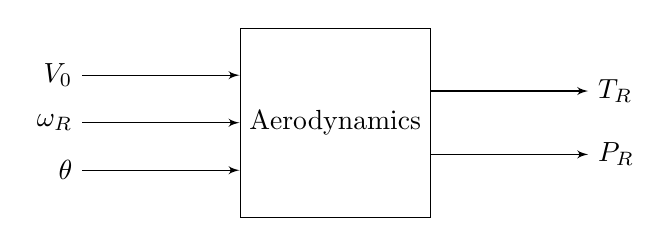
\begin{tikzpicture}[auto, node distance=2.5cm,>=latex']
  
  \node (adc) [draw,minimum size=24mm] {Aerodynamics};
  \path (adc.north west)--(adc.south west) foreach \j in {1,...,3} {  coordinate [pos=.25*\j] (y\j)};
  
   \foreach \i/\name  in {1/$V_0$,2/$\omega_R$,3/$\theta$}  
   \draw[<-] (y\i) -- ++(-2,0) node[left] (x\i){\name};

  \path (adc.north east)--(adc.south east) foreach \j in {1,...,2} {coordinate [pos=1/3*\j] (z\j)};
\foreach \i/\name  in {1/$T_R$,2/$P_R$} 
    \draw[->] (z\i) -- ++(2,0) node[right] (t\i){\name};

\end{tikzpicture}
  \caption{Logical block representing the aerodynamics}
  \label{fig:d_aerodynamic_block}
\end{figure}

In the block the actual \acrshort{TSR} is firstly computed, then the power coefficient is extracted from the lookup table obtained from the \autoref{subsec:lookup_cp} and finally the rotor torque is obtained by dividing the rotor power (expressed as in \autoref{eq:power}) by the rotor speed:
\begin{equation}
    T_R = \frac{P_R}{\omega_R} \ \ \left[\si{\newton\per\meter}\right]
\end{equation}

\subsection{Pitch actuation}
In order to model the dynamic of the mechanical pitch actuators, two main effects have to be taken into account. The first one is the transfer function delaying the real response compared to the command action, while the second one is the maximum pitching rate. 
\begin{figure}[htb]
  \centering
  \tikzstyle{block} = [draw, fill=white, rectangle, 
    minimum height=2.5em, minimum width=3em]
\tikzstyle{sum} = [draw, fill=white, circle, node distance=1cm]
\tikzstyle{input} = [coordinate]
\tikzstyle{output} = [coordinate]
\tikzstyle{pinstyle} = [pin edge={to-,thin,black}]

\begin{tikzpicture}[auto, node distance=2.5cm,>=latex']
  \node [input, name=input] {};
  \node [block, right of=input, minimum size=24mm] (main) {Pitch actuator};
  \node [output, right of=main] (output) {};

  \draw [->] (input) -- node {$\theta^*$} (main);
  \draw [->] (main) -- node {$\theta$} (output);
\end{tikzpicture}
  \caption{Logical block representing the pitch actuator}
  \label{fig:d_pitch_actuator_block}
\end{figure}

The simplest mechanical model has a second order dynamic, as suggested by \cite{Olimpo_Anaya‐Lara}:
\begin{equation}
    \frac{\beta}{\hat{\beta}}=\frac{\omega_p^2}{s^2+2\zeta_p\omega_p s+\omega_p^2}
    \label{eq:beta_TF}
\end{equation}
with $\zeta_p=0.7$ and $\omega_p=2\pi \left[\si{\radian}\right]$ provided by the same reference.\\
The maximum pitching rate is reported to be $\pm 9 \left[\si{\degree\per\second}\right]$ in \cite{Olimpo_Anaya‐Lara}, and $\pm 10 \left[\si{\degree\per\second}\right]$ in \cite{Aerodynamics_of_wind_turbines} and \cite{DTU_Wind_Energy_Report-I-0092}. In this simulation, a rate limiter block with threshold at $\pm 10 \left[\si{\degree\per\second}\right]$ is placed after the actuation block.

\subsection{Mechanical transmission}
\begin{figure}[htb]
  \centering
  \tikzstyle{block} = [draw, fill=white, rectangle, 
    minimum height=2.5em, minimum width=3em]
\tikzstyle{sum} = [draw, fill=white, circle, node distance=1cm]
\tikzstyle{input} = [coordinate]
\tikzstyle{output} = [coordinate]
\tikzstyle{pinstyle} = [pin edge={to-,thin,black}]

\begin{tikzpicture}[auto, node distance=2.5cm,>=latex']
  \node [input, name=input] {};
  \node [block, right of=input, minimum size=24mm, align=center] (main) {Mechanical \\ transmission};
  \node [output, right of=main] (output) {};

  \draw [->] (input) -- node {$\omega_R$} (main);
  \draw [->] (main) -- node {$\omega_G$} (output);
\end{tikzpicture}
  \caption{Logical block representing the mechanical transmission}
  \label{fig:d_mechanical_transmission_block}
\end{figure}
In this simple simulation, the transmission ratio is unitary, and so the relationship between the the rotational speed of the rotor $\omega_{R}$ and the generator $\omega_{G}$ is:
\begin{equation}
    n = \frac{\omega_{R}}{\omega_{G}} = \frac{1}{1}
    \label{eq:transmission_ratio}
\end{equation}
In this configuration the turbine is assumed to be direct drive, but a general n is considered in the derivations for making it more general.

\subsection{Dynamical equation}
\begin{figure}
  \centering
  \tikzstyle{output} = [coordinate]

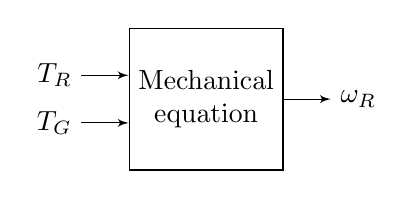
\begin{tikzpicture}[auto, node distance=2.5cm,>=latex', scale=0.3]
  
  \node (adc) [draw,minimum size=18mm,align=center] {Mechanical \\ equation};
  
  \path (adc.north west)--(adc.south west) foreach \j in {1,...,2} {  coordinate [pos=1/3*\j] (y\j)};
  
   \foreach \i/\name  in {1/$T_R$,2/$T_G$}  
   \draw[<-] (y\i) -- ++(-2,0) node[left] (x\i){\name};

   \path (adc.north east)--(adc.south east) foreach \j in {1,...,1} {coordinate [pos=1/2*\j] (z\j)};
  \foreach \i/\name  in {1/$\omega_R$} 
    \draw[->] (z\i) -- ++(2,0) node[right] (t\i){\name};

\end{tikzpicture}
  \caption{Logical block representing the mechanical equation}
  \label{fig:d_mech_equation_block}
\end{figure}
The dynamical equation block solves the Newton's law written on the rotor side of the transmission:
\begin{equation}
    \begin{cases}
      J_R \dot{\omega^R} = T_R^R - B_R\omega^R - T_T^R\\
      J_G \dot{\omega^G} = T_T^G - B_G\omega^G - T_G^G\\
      T_T^R\omega^R = T_T^G\omega^G\\
    \end{cases}
\end{equation}
This system of equations may be solved and finally the mechanical dynamic equation can be written on the rotor side:
\begin{gather}
    \left(J_R + \frac{J_G}{n^2}\right) \dot{\omega^R} = T_R^R - \frac{T_G^G}{n} - \left(B_R + \frac{B_G}{n^2}\right)\omega^R \\
    J_{eq} \dot{\omega^R} = T_R^R - T_G^R - B_{eq}\omega^R
    \label{eq:mech_eq}
\end{gather}
Where the subscript indicates if the quantity is referred to the rotor or to the generator, while the apex indicates the side of the transmission in which it is expressed.

\subsection{Transmission damping}
Finding information on the mechanical damping is not simple because it is a parameter difficult to be identified via simulations only, and so real measurements would be required. Since a value of B is necessary to make the simulation more realistic (at least conceptually) then the system of equations in \autoref{eq:damping_sys} may be set up to try to recover it. The former equation is the power balance between rotor and generator side of the transmission, while the latter is the torque balance:
\begin{gather}
\left\{
\begin{aligned}
\eta T_R^R \omega^{R} = T_G^G\omega^{G} \\
T_G^R =T_R^{R} - B_{eq}^R \omega^R
\end{aligned}
\right. ;
\left\{
\begin{aligned}
T_G^G\frac{\cancel{\omega^{R}}}{n}=\eta T_R^R \cancel{\omega^{R}} \\
\frac{T_G^G}{n}=T_R^R-B_{eq}^R\omega^R
\end{aligned}
\right. ;
\left\{
\begin{aligned}
T_G^G = \eta n T_R^R \\
\eta T_R^R\frac{\cancel{n}}{\cancel{n}} = T_R^R-B_{eq}^R\omega^R
\end{aligned}
\right. 
\label{eq:damping_sys}\\
B_{eq}^R= \frac{T_R^R}{\omega^R}(1 - \eta)= \frac{K_{opt}(\omega^R)^2}{\omega^R}(1 - \eta) = K_{opt}\omega^R(1 - \eta) \ \ \mesunt{\kilo\gram\square\meter}
\label{eq:damping}
\end{gather} 
where the coefficient $K_{opt}$ is a coefficient that will be later introduced in \autoref{subsec:torque_reference}, and has the units of $\mesunt{\newton \meter \square\second }$.\\
It could be noticed that, for a chosen value of efficiency $\eta$, then the damping in \autoref{eq:damping} depends on the rotational speed. Furthermore, it is also possible that the efficiency itself depends on the rotational speed, and so it is not possible to build a real map between these quantities with only the literature information at our disposal. To solve this problem, two assumptions are done. The first one is that the efficiency is not speed dependent and so only one value may be used as representative for all the operative conditions. In particular, the efficiency $\eta = 0.954$ is chosen, as proposed by \cite{Olimpo_Anaya‐Lara}. The second one is to consider the rated rotational speed. With these assumptions in mind, the damping becomes:
\begin{equation}
  B_{eq}^R = K_{opt}\omega^R(1 - \eta) = 1.02\cdot10^7 1.014(1 - 0.954)=475.76 \cdot 10^3 \ \ \mesunt{\kilo\gram\square\meter}
\end{equation}

\subsection{Electrical generator}
\begin{figure}[htb]
  \centering
  \tikzstyle{block} = [draw, fill=white, rectangle, minimum height=2.5em, minimum width=3em]
\tikzstyle{sum} = [draw, fill=white, circle, node distance=2.0cm]
\tikzstyle{input} = [coordinate]
\tikzstyle{output} = [coordinate]
\tikzstyle{pinstyle} = [pin edge={to-,thin,black}]
\tikzset{
dot/.style = {circle, fill, minimum size=#1,
              inner sep=0pt, outer sep=0pt},
dot/.default = 4pt % size of the circle diameter 
}

\usetikzlibrary{positioning}
\makeatletter
\pgfdeclareshape{record}{
\inheritsavedanchors[from={rectangle}]
\inheritbackgroundpath[from={rectangle}]
\inheritanchorborder[from={rectangle}]
\foreach \x in {center,north east,north west,north,south,south east,south west}{
\inheritanchor[from={rectangle}]{\x}
}
\foregroundpath{
\pgfpointdiff{\northeast}{\southwest}
\pgf@xa=\pgf@x \pgf@ya=\pgf@y
\northeast
\pgfpathmoveto{\pgfpointadd{\southwest}{\pgfpoint{-0.33\pgf@xa}{-0.6\pgf@ya}}}
\pgfpathlineto{\pgfpointadd{\southwest}{\pgfpoint{-0.75\pgf@xa}{-0.6\pgf@ya}}}
\pgfpathlineto{\pgfpointadd{\northeast}{\pgfpoint{-0.75\pgf@xa}{-0.6\pgf@ya}}}
\pgfpathlineto{\pgfpointadd{\northeast}{\pgfpoint{-0.33\pgf@xa}{-0.6\pgf@ya}}}
}
}
\makeatother

\begin{tikzpicture}[auto, node distance=2.5cm,>=latex']
  \node [style=input] (1) at (0, 0.65) {};
  \node [style=input] (2) at (-0.75, -1.5) {};
  \node [style=input] (6) at (0.75, 0.65) {};
  \node [style=input] (9) at (0.75, -0.65) {};
  \node [style=input] (10) at (5.75, 0) {};
  \node [style=input] (11) at (8.25, -1.5) {};
  \node [style=input] (12) at (9.25, -1.5) {};

  \node [style=block, minimum size=24mm] (3) at (2, 0) {Controller};
  \node [style=block, minimum size=24mm] (4) at (7, -0.75) {Generator};

  \node [dot=1pt] (5) at (8.5, 2) {};
  \node [dot=1pt] (7) at (5.75, -1.5) {};
  \node [dot=1pt] (8) at (0, -1.5) {};

  \draw [-] (4) -| node {} (5);
  \draw [-] (5) -| node {} (1);
  \draw [->] (1) -- node {$P_G$} (6);

  \draw [->] (3) -- node {$T^{*}_{G}$} (10);

  \draw [-] (2) -- node {$\omega_G$} (8);
  \draw [->] (8) -- node {} (7);
  \draw [->] (8) |- node {} (9);
  \draw [->] (11) -- node[pos=0.95] {$T_G$} (12);

  % \node [style=block] (1) at (3, 0) {Aero};
  % \node [style=block, align=center] (2) at (6, 0) {Mech. \\ dynamic};
  % \node [style=block] (3) at (3, -2.5) {Mechanical \\ transmission};
  % \node [style=block, align=center] (4) at (6, -2.5) {Pitch \\ controller};
  % \node [style=block, align=center] (5) at (9, -2.5) {Pitch \\ actuator};
  % \node [style=block, align=center] (6) at (6, -4) {Torque \\ controller};
  % \node [style=block] (7) at (9, -4) {Generator};
  % \node [style=block, align=center] (8) at (12, -4) {Power \\electronics};
  % \node [style=block] (9) at (15, -4) {Grid};
  % \node [style=input] (10) at (1.5,0.35) {};
  % \node [dot=1pt] (11) at (1.25, -2.5) {};
  % \node [dot=1pt] (12) at (7.5, 1) {};
  % \node [dot=1pt] (13) at (1.25, 1) {};
  % \node [dot=1pt] (14) at (10.25, -1.5) {};
  % \node [dot=1pt] (15) at (2, -1.5) {};
  % \node [dot=1pt] (17) at (4.5, -2.5) {};
  % \node [dot=1pt] (18) at (10.5, -4) {};
  % \node [dot=1pt] (19) at (4.5, -0.75) {};

  % \draw [->] (10) -- node {$V_0$} (1.150);
  % \draw [->] (11) -- node {$\omega_R$} (3);
  % \draw [-] (11) -- node {} (13);
  % \draw [->] (1.160) ++(1.15,0) -- node {$T_R$} (2.165);
  % \draw [-] (2) -| node {} (12); 
  % \draw [-] (12) -- node {} (13);
  % \draw [->] (13) |- node {} (1.175);
  % \draw [->] (3) -> node {$\omega_G$} (4);
  % \draw [->] (4) -> node {$\hat{\theta}$} (5);
  % \draw [-] (5) -| node {} (14);
  % \draw [-] (15) -- node {$\theta$} (14);
  % \draw [->] (15) |- node {} (1.200);
  % \draw [-] (17) |- node {} (6);
  % \draw [->] (6) -- node {$\hat{T}_G$} (7);
  % \draw [->] (7) -> node[below] {$P_G$} (8);
  % \draw [-] (18) |- node {} (19);
  % \draw [->] (19) |- node {$T_G$} (2.200);
  % \draw [->] (8) -> node {$P_{GE}$} (9);

\end{tikzpicture}
  \caption{Logical block representing the generator and its controller}
  \label{fig:d_generator_block}
\end{figure}

As said before, nowadays the Permanent Magnet Syncronous Machines (PMSM) are the most commonly employed generators, and so they are going to be studied in this work.\\
In this work the isotropic \acrshort{PMSM} are taken into account. For studying them it is convenient to project the fundamental equations from a reference frame fixed in the stator windings (named \textit{abc}) in a reference frame synchronous with the rotor, named \textit{dq frame}, in which the alternate electrical quantities of voltage and current are represented as their amplitude values. 
In this frame the equations of the machine are:
\begin{gather}
  0=u_d-L_{s}i_q\omega_{me}+L_{s}\frac{di_d}{dt}+R_{s}i_d 
  \label{eq:d_axis_eq}\\
  \omega_{me}\Lambda_{mg}=u_q+L_{s}i_d\omega_{me}+L_{s}\frac{di_q}{dt}+R_{s}i_q
  \label{eq:q_axis_eq}
\end{gather}
where $u_d$ and $u_q$ are the voltage of the d- and q-axis expressed in the dq frame (i.e. the peak value of the respectively quantities in the abc frame), $i_d$ and $i_q$ are the current in the dq frame (transformed in the same way as the the voltage), $\omega_{me}$ is the electro-mechanical speed of the rotor ($\omega_{me}=p\omega$, with $p$ the number of pole pairs and $\omega$ the mechanical rotational speed $\mesunt{\radian \per \second}$), $L_{s}$ is the inductance and $R_{s}$ the resistance of the stator, $\Lambda_{mg}$ is the flux linkage of the permanent magnets.\\
By multiplying both sides of \autoref{eq:d_axis_eq} by $i_d$, \autoref{eq:q_axis_eq} by $i_q$, and then summing them together is it possible to obtain the following power balance:
\begin{equation}
  p\omega\Lambda_{mg}i_q=u_di_d + u_qi_q+ L_{s}\left(i_d\frac{di_d}{dt} + i_q\frac{di_q}{dt}\right) + R_{s}(i_d^2 + i_q^2)
  \label{eq:gen_power_balance}
\end{equation}
Since in isotropic machines the relationship between a given input torque and the corresponding \textit{q-axis} current is univocal (i.e. the $\textit{q-axis}$ does not play any role in the conversion of the torque) it is convenient to keep the total current as low as possible in order to minimize the joule losses. This is achieved by working in the so called \acrfull{MTPA} regime, in which the current on the \textit{d-axis} is null. For this reason, knowing that the quadrature axis controller ensures $i_d=0 \, \mesunt{\ampere}$ one can rewrite:
\begin{equation}
  \underbrace{p\omega\Lambda_{mg}i_q}_{Mech. IN} = \underbrace{u_qi_q}_{Elec. OUT}+ \underbrace{L_{s} i_q\frac{di_q}{dt}}_{Inductance} + \underbrace{R_{s}i_q^2}_{Joule}
  \label{eq:gen_power_balance2}
\end{equation}
Since the power is not invariant in the transformation from the abc frame to the dq but $P_{dq} = \frac{3}{2}P_{abc}$, \autoref{eq:gen_power_balance2} has to be rewritten as:
\begin{equation}
  P_G = T_G\omega = \frac{3}{2}p\omega\Lambda_{mg}i_q = \frac{3}{2}u_qi_q + \frac{3}{2}L_{s} i_q\frac{di_q}{dt} + \frac{3}{2}R_{s} i_q^2
  \label{eq:gen_power_balance3}
\end{equation}
The choice of this frame makes the system of equations describing the generator linear, so the two axis can be controlled as two separated \acrfull{SISO} systems. In particular, the torque control is achieved by regulating the current of the q-axis, and letting the controller of the d-axis ensuring $i_d=0 \, \mesunt{\ampere}$.
\begin{figure}[htb]
\centering
\tikzstyle{block} = [draw, fill=white, rectangle, 
    minimum height=2.5em, minimum width=3em]
\tikzstyle{sum} = [draw, fill=white, circle, node distance=1cm]
\tikzstyle{input} = [coordinate]
\tikzstyle{output} = [coordinate]
\tikzstyle{pinstyle} = [pin edge={to-,thin,black}]

\begin{tikzpicture}[auto, node distance=1.8cm,>=latex']

    \node [input, name=input] {};
    \node [sum, right of=input] (sum) {};
    \node [block, right of=sum] (controller) {$R_{iq}$}; % controller
    \node [block, right of=controller, node distance=2cm] (G_c) {$\frac{1}{1+\uptau_{c}s}$}; % elecrical delay
    \node [sum, right of=G_c, node distance=2cm] (sum2) {};
    \node [block, right of=sum2] (sys2) {$\frac{-1}{sL_{s}+R_{s}}$};
    \node [block, right of=sys2, node distance=2.3cm] (sys3) {$\frac{3}{2}p\Lambda_{mg}$};
    \node [sum, right of=sys3, node distance=2cm] (sum3) {};
    \node [block, right of=sum3, node distance=2cm] (sys4) {$\frac{-1}{B_{eq}+sJ_{eq}}$};
    \node [block, below of=sys2, node distance=2cm] (sys5) {$p\Lambda_{mg}$};
    \node [input, name=T_L, above of=sum3] {};
    \node [pinstyle, name=pin1, below of=G_c] {};
    
    \draw [->] (controller) -- node[name=u] {$U_q^{*'}$} (G_c);
    \node [output, right of=sys4] (output) {};
    %\node [block, below of=u] (measurements) {Measurements};
    \coordinate [below of=u, node distance=1.5cm] (measurements) {};
    \coordinate [above of=sum3] (tl) {};

    \draw [draw,->] (input) -- node {$I_q^*$} (sum);
    \draw [->] (sum) -- node {} (controller);
    \draw [->] (G_c) -- node [] {$U_q'$}(sum2);
    \draw [->] (sum2) -- node [name=sum2sys2] {} (sys2);
    \draw [->] (sys2) -- node [name=sys2sys3] {$I_q$} (sys3);
    \draw [->] (sys3) -- node [name=sys3sum3] {$T_G$} (sum3);
    \draw [-] (sys2sys3) |- (measurements); 
    \draw [->] (measurements) -| node [pos=0.9] {$-$} (sum); 
    \draw [->] (sum3) -- node [name=sum3sys4] {} (sys4);
    \draw [->] (sys4) -- node [name=sys4output] {$\Omega_G$} (output);
    \draw [->] (sys5) -| node [name=sys5sum2] [pos=0.95] {$-$} (sum2);
    \draw [->] (sys4output) |- node [near end] [name=outputsys5] {} (sys5);
    \draw [draw, ->] (T_L) -- node[pos=0.9] {$-$} node {$T_{R}$} (sum3);

    %\draw [->] (G_c) -- node [name=U_q] {$U_q'$}(output);
    %\draw [->] (y) |- (measurements);
    
    %\draw [-] (U_q) |- (measurements);
    
    %\draw [->] (measurements) -| node[pos=0.95] {$-$} 
    %\draw [->] (sys2sys3) |- {$y_m$} (sum);
        
    %\draw [->] 
\end{tikzpicture}

\caption{Block diagram of the q-axis current control of a PMSM}
\label{fig:PMSM}
\end{figure}

\autoref{fig:PMSM} represents the block diagram of q-axis current control of a \acrshort{PMSM}, coupled with also the mechanical equation. $R_{iq}$ is the controller, $\uptau_{c}$ $\left[\si{\second}\right]$ is the time delay of the power electronic converter, $T_R \ \left[\si{\newton \per \meter}\right]$ is the torque imposed by the wind on the rotor.\\
It could be seen that the aerodynamical torque $T_R$ enters as a disturb in the block diagram. This model is not a description of the real behavior of the \acrshort{WT}, because the $T_R$ is affected by the $\Omega_G$, and so in principle some sort of interaction between these quantities should have been introduced. Unfortunately, this dependency is not linear, implying that it is not possible to find a transfer function between them, and furthermore (and more important from the theoretical point of view) that the Laplace domain techniques are not valid any more. This problem may be solved observing that this mechanical dynamic evolves slowly compared to the electrical one, and so the latter sees the former as an almost-constant disturb. Finally for the sake of completeness, it must be remembered that the interactions between rotational speed and aero torque is taken into account into the aerodynamical block of the simulation as could be seen in the schema of the whole plant at \autoref{fig:d_plant_schema}. \textcolor{red}{Vedere se il riferimento allo schema di tutto l'impianto è introdotto in modo corretto, cioè se aiuta a far capire meglio il concetto che si vuole esprimere}\\

 Obtaining the electrical parameters of commercial generators is not an easy task because they are protected by the manufacturers. For this reason, the values used by \cite{10-MW_Direct-Drive_PMSG-Based_Wind_Energy_Conversion_System_Model} and reported in \autoref{tab:generator_parameter} are employed in this simulation.
\begin{table}[htb]
    \caption{Parameters for the \acrlong{PMSM} generator presented by \cite{10-MW_Direct-Drive_PMSG-Based_Wind_Energy_Conversion_System_Model}}
    \centering
    \begin{tabular}{lccc}
    \toprule
    Parameter & Value & & Source\\ \midrule
    Inertia & 4800 & $\left[\si{\kilo\gram\square\meter}\right]$ & \cite{the_switch_datasheet} \\ \midrule	
    Poles & 320 & & \multirow{5}{*}{\cite{10-MW_Direct-Drive_PMSG-Based_Wind_Energy_Conversion_System_Model}} \\
    \textit{q-axis} inductance & 1.8 & $\left[\si{\milli\henry}\right]$ & \\
    \textit{d-axis} inductance & 1.8 & $\left[\si{\milli\henry}\right]$ &\\
    Stator resistance & 64 & $\left[\si{\milli\ohm}\right]$ &\\
    Magnets flux & 19.49 & $\left[\si{\weber}\right]$ &\\ \midrule
    Friction & 0 & $\left[\si{\kilo\gram\square\meter\per\second}\right]$ & \\
    Time delay introduced by the convert & 500 & $\left[\si{\micro\second}\right]$ & \\
    Inverter switching frequency & 1 & $\mesunt{\kilo\hertz}$ & \\
    \bottomrule
    \end{tabular}
    \label{tab:generator_parameter}
\end{table}

% The Simulink implementation of the control loop presented in \autoref{fig:d_torque_control} is reported in \autoref{fig:iq_control}.
% \begin{figure}[htb]
%    \centering
%    \includegraphics[width=0.8\textwidth]{images/iq_control.png}
%    \caption{Feedback scheme of the \textit{q-axis} control loop}
%    \label{fig:iq_control}
% \end{figure}
The friction has been considered $ 0 \, \mesunt{\kilo\gram\square\meter\per\second}$ because it has been already considered in the equivalent one of the transmission. \\
 Once the inverter switching frequency is defined \textcolor{blue}{where can I find some references justifying this choice? pag 112 reference}, then we can base on it the definition of the $\uptau_c$ and bandpass frequency. As described in \autoref{subsec:PMSM_control}, the time delay introduced by it in the response (i.e. the one used in the $G_c=\frac{1}{1+s\uptau_c}$ block of \autoref{fig:d_torque_control}) may be computed as half the switching period:
 \begin{gather}
 \uptau_{c}=\frac{\frac{1}{f_{inverter}}}{2}=\frac{\frac{1}{1000}}{2}=500 \ \ \mesunt{\micro \second}
 \end{gather}
 In more detail, the $\uptau_c$ is a delay introduced by the analog PWM modulator controlling the electrical machine. Assuming that the converter samples input signals and acts its switches synchronously, then the propagation time from the input to the output of the command signal is bounded between two extreme conditions. On one hand, if the change of the input happens at a time instant slightly before the sampling one it will be immediately detected and the corresponding output value will be provided as output almost immediately, while on the other hand, when the change happens slightly after the sampling instant, then the output will be propagated after an entire cycle. To average these two situations, a propagation delay equal to half of the converter period may be assumed. In case of a digital converter, the analog to digital and digital to analog conversions have to be taken into account and so the delay increased, usually of 1.5 the switching delay.
 
 \subsubsection{Extension of the static power curve}\label{subsec:genertaor_power_curve}
 Now that the generator's characteristics have been introduced, it is possible to extend the static power curve presented in \autoref{subsec:static_power_curve} taking into account the electrical losses.These curves can be found starting from \autoref{eq:gen_power_balance3} and considering that the time derivative are null. The steady state current and voltage can be found thanks to \autoref{eq:q_axis_eq}. The powers as function of the \acrshort{WS} are reported in \autoref{fig:fig_static_electro_power}, considering both unity and lower efficiency.
\begin{figure}[htb]
  \centering
  \includegraphics[width=0.65\textwidth]{images/vectorial/fig_static_electro_power.eps}
  \caption{Incoming mechanical, outgoing electrical, and lost power as function of the WS}
  \label{fig:fig_static_electro_power}
\end{figure}

 
\newpage
\newpage
\section{Control of the basic model}\label{sec:c_basic_model_control}

\subsection{Generator's torque reference synthesis}\label{subsec:torque_reference}
As presented in \cite{Aerodynamics_of_wind_turbines} and \cite{SMILDEN2016386}, the generator's torque reference is computed starting from the rotational speed of the shaft. \\
As said before, below rated wind speed the objective is to ensuring the maximum power extraction, and so working with the maximum power coefficient:
\begin{gather}
    T_G=\frac{P_G}{\omega_G}=\frac{\frac{1}{2}\rho c_{P,MAX} \pi R^2 V_0^3}{\omega_G} \ \ \left[\si{\newton\per\meter}\right]
    \label{eq:T_G1}
\end{gather}
then the \acrshort{WS} can be rewritten as
\begin{equation}
    \lambda_{opt} = \frac{\omega_R R}{V_0} = \frac{n \omega_G R}{V_0} \Rightarrow V_0=\frac{n\omega_G R}{\lambda_{opt}}  \ \ \left[\si{\meter\per\second}\right]
    \label{eq:lambda_opt}
\end{equation}
By replacing \autoref{eq:lambda_opt} into \autoref{eq:T_G1} then the drivetrain torque expressed on the generator side is:
\begin{equation}
    T^G=\frac{P_G}{\omega_G^G}=\frac{\frac{1}{2}\rho c_{P,MAX} \pi R^2 \left(\frac{n\omega_G R}{\lambda_{opt}}\right)^3}{\omega_G^G} = \frac{\rho c_{P, MAX} \pi R^5 }{2 \lambda_{opt}^3}n^3\omega_G^{G \ 2} = K_{opt}n^3\omega_G^{G \ 2}  \ \ \left[\si{\newton\per\meter}\right]
    \label{eq:T_G2}
\end{equation}

\begin{table}[htb]
    \centering
    \begin{tabular}{ccc}
    \toprule
         & $\omega^R$ & $\omega^G$  \\ \midrule
         P & $K_{opt} \left(\omega^{R}\right)^3$ & $K_{opt}\left(n \omega^{G}\right)^3$\\
         $T^R$ & $K_{opt} \left( \omega^{R}\right)^2$ & $K_{opt}\left(n \omega^{G}\right)^2$\\
         $T^G$ & $K_{opt} n \left(\omega^{R}\right)^2$ &  $K_{opt} n^3\left(\omega^{G}\right)^2$\\ \bottomrule
    \end{tabular}
    \caption{Map for the use of torque constant}
    \label{tab:gain_map}
\end{table}

 For the differences discussed above, there is a small difference between the $K_{opt}$ proposed from \cite{DTU_Wind_Energy_Report-I-0092} and the one computed by me, and again the one compute will be used in the simulation:
 \begin{gather*}
     K_{opt, report} = 1.001 \cdot 10^7 \ \ \ \left[\si{\newton\meter\square\second}\right] \\
     K_{opt, computed} = 1.020 \cdot 10^7 \ \ \ \left[\si{\newton\meter\square\second}\right] 
 \end{gather*}

Above rated wind speed the objective is to keep the constant rotational speed and so the command:
\begin{equation}
    T_G = \frac{P_{rated}}{\omega_{rated}^G} = \frac{nP_{rated}}{\omega_{rated}^R}\ \ \left[\si{\newton\per\meter}\right]
    \label{eq:T_G3}
\end{equation}
is given.\\
In the Simulink model the implementation of the generator's torque reference is done employing a proportional and a saturation blocks, limiting the torque when it goes above the rated speed.
\begin{figure}[htb]
    \centering
    \includegraphics[width=0.7\textwidth]{images/torque_control.png}
    \caption{Simulink block diagram for the torque control}
    \label{fig:torque_control}
\end{figure}

\subsection{Pitch controller}
In this simple model, the \textit{collective} pitching strategy is employed, meaning that all the blades are rotated of the same quantity.\\
As suggested in \cite{Aerodynamics_of_wind_turbines} and \cite{SMILDEN2016386}, the pitch controller has two different behaviours in the operational regions, and so in a wide sense it is a non-linear one: below rated \acrshort{WS}, it has not to be activated at all, while in the full load region it has to pitch the blade in order to drive the rotational speed to rated value. Its implementation is done as reported in \autoref{fig:pitch_control}.
\begin{figure}[htb]
    \centering
    \includegraphics[width=\textwidth]{images/pitch_control_2.png}
    \caption{Block diagram of the pitch controller\textcolor{red}{Update this picture}}
    \label{fig:pitch_control}
\end{figure}

The core part of the controller is a \acrfull{PI} action driven by the speed error defining the pitch angle. A saturation block on the pitch angle is used to impose the mechanical constraints, so to limit the blade rotation: $\theta \in \left[0, 90\right] \si{\degree}$. This threshold prevents that a negative speed error produces a pitching towards stalling.

The tuning of this PI is not straightforward because the system to be controlled is not linear, and so the standard techniques cannot be implemented. In particular, at high wind speeds the aerodynamic loads are more sensitive to changes in the angles of attack, and so the change in pitch should be limited \cite{Aerodynamics_of_wind_turbines}. A possible solution is to schedule the gain during the operation of the mechanism.

\subsubsection{Simplified approach from literature}\label{subsec:gain_poly}
Since these aerodynamic considerations are out of the scope of this thesis, a simplified approach is followed, according what is presented in \cite{Olimpo_Anaya‐Lara}: the turbine is treated as a linear varying-parameter system and the gains are scheduled according to one state of the system itself. This is an advantageous choice, because the approach simplifies the description of the system and does not require a lot of measurements, but on the other hand it does not fully represent it. Under these considerations, \cite{Olimpo_Anaya‐Lara} proposes to schedule the gains based on a measurement of the pitch angle itself, meaning that the $\theta$ is taken as state representing the entire \acrshort{WT}, including the effective \acrshort{WS}. Specifically for the DTU 10 MW, \cite{Olimpo_Anaya‐Lara} proposes the schedule based on the polynomials in \autoref{eq:k_p_poly} and \ref{eq:k_i_poly}:
\begin{gather}
    k_p(\theta)=1.000-2.541 \ \theta-7.814 \ \theta^2+46.281 \ \theta^3-59.871 \ \theta^4
    \label{eq:k_p_poly}\\
    k_i(\theta)=0.351-2.405 \ \theta+13.128 \ \theta^2-31.926 \ \theta^3+27.689 \ \theta^4
    \label{eq:k_i_poly}
\end{gather}
with $\theta$ in $\left[\si{\radian}\right]$. For a more practical visualization these polynomials have been plotted in \autoref{fig:fig_gain_schduling}, where it can be seen that a great variation of the coefficients happens in between the minimum and maximum angles. \textcolor{red}{Write how does they have compute these polynomials}\\
\begin{figure}
    \centering
    \includegraphics[width=0.6\textwidth]{images/fig_gain_scheduling.png}
    \caption{Proportional and integral gains for blade's controller as function of pitch angle, simplified approach from \cite{Olimpo_Anaya‐Lara}}
    \label{fig:fig_gain_schduling}
\end{figure}

Another option could have been to schedule the pitch based on the \acrshort{WS} itself, but this would have required a direct measurement of the resource. \\
As final remark, it must be noted that using the actual pitch angle as scheduling variable, implies that 
the controller dynamic are not slower compared to the system itself and so it may not behave exactly as expected in the vicinity of the rated wind speed.

\subsubsection{Gain scheduling based on the aerodynamics}\label{subsec:gain_schdeuling_NREL5MW}

As described in \cite{Aerodynamics_of_wind_turbines}, \cite{NREL_5MW_reference}, and \cite{ris_r_1500} applying a linearization of the \autoref{eq:mech_eq} and further mathematical manipulations that are out of the scope of this thesis, the gains may be expressed in close form as :
\begin{gather}
    k_P(\theta) = \frac{2J_{eq}\omega_{rated}\zeta_{\Phi}\omega_{\Phi\eta}}{\frac{1}{n}\left(-\frac{dP(\theta)}{d\theta}\right)\vert_{\theta=0}}GK(\theta)
    \label{eq:kp}\\
    k_I(\theta) = \frac{J_{eq}\omega_{rated}\omega_{\Phi\eta}^2}{\frac{1}{n}\left(-\frac{dP(\theta)}{d\theta}\right)\vert_{\theta=0}}GK(\theta)
    \label{eq:ki}\\
    GK(\theta) = \frac{1}{1+\frac{\theta}{\theta_K}} \label{eq:GK}
\end{gather}
where $J_{eq}$ is the inertia of the drivetrain on the low speed shaft, $\omega_{rated}$ is the rotational speed of the low speed shaft at rated power, n is the gear ratio, $\zeta_{\Phi}$ and $\omega_{\Phi\eta}$ are the damping ratio and the resonant frequency of the dynamic response of the PI-regulator. \cite{NREL_5MW_reference} suggests to take $\omega_{\Phi\eta}=0.6\mesunt{\radian\per\second}$ and $0.6<\zeta_{\Phi}<0.7$. The most complicated term to be computed is the sensitivity of the power w.r.t. the pitch angle $-\frac{dP}{d\theta}$. Its estimation should be done applying a steady \acrshort{BEM} (also known as \textit{Frozen wake BEM}) as reported in \cite{Aerodynamics_of_wind_turbines} or with specific software. \\
The procedure for computing these gains is implemented and validated on the NREL 5 MW turbine, since more intermediate steps are present in the literature. After the validation, the same steps are repeated using the aerodynamical properties of the DTU 10 MW blades. \\
The frozen wake BEM is implemented in two steps, then repeated for all the windspeeds between the rated and the cut out one. In the first one, the standard BEM presented in \textcolor{red}{write where it was presented} is applied on the blade, considering that it is pitched as to produce the rated power (i.e. the pitch angle is the one scheduled in \textcolor{red}{Write where the pitch angle is scheduled}). In this step the induction coefficients \textit{a} and \textit{$a_{prime}$} (\textcolor{red}{See if this are called in the same way when the BEM is presented and if they are written with the correct font}) found are stored. In the second step, the previously described BEM is applied but the pitch angle is changed on a set around the optimal one, while the induction coefficients are kept constant (i.e. they are not computed with the iterative procedure). The power is then computed for each pitch angle and finally the power derivative wrt the pitch angle is obtained applying the finite difference method.
\subsubsection{Validation of the procedure on the NREL 5MW}
In order to validate the procedure, this described procedure is applied on the NREL 5MW turbine.\\
The derivative of the power computed at the expected pitch angle is  reported in \autoref{fig:fig_dPdtheta}, alongside its interpolation done by a first and second order polynomials. It could be seen that the second order approximation seems to better follow the tendency of the computed points with respect to the first order one. 
\begin{figure}[htb]
    \centering
    \includegraphics[width=0.6\textwidth]{images/fig_dPdtheta.eps}
    \caption{Aerodynamic power gain for the NREL 5MW WT}
    \label{fig:fig_dPdtheta}
\end{figure}

The interpolations are used to find two important parameters, called $\theta_{K}$ and  $-\frac{dP(\theta)}{d\theta}\vert_{\theta=0}$. The first is the blade-pitch angle at which the pitch sensitivity has doubled from its value at the rated operating point, while the second is the pitch sensitivity at 0 pitch (i.e. the intercept of the interpolation). For the turbine under investigations, these two parameters are $\theta_K=10.25 \mesunt{\degree}$ and  $\frac{dP(\theta)}{d\theta}\vert_{\theta=0} = -29.15 \mesunt{\mega\watt\per\radian}$, while the ones reported in the report are $\theta_K=6.3 \mesunt{\degree}$ and  $-\frac{dP(\theta)}{d\theta}\vert_{\theta=0} = -25.52\mesunt{\mega\watt\per\radian}$ (for the linear case). These values seems to be reasonably close each other.\\ 
Once all the terms in \autoref{eq:ki}, \ref{eq:kp}, and \ref{eq:GK} are available and the gain scheduling can be determined, and the comparison reported in \autoref{fig:fig_gain_pitch}.
\begin{figure}[htb]
    \centering
    \includegraphics[width=0.6\textwidth]{images/fig_gain_pitch.eps}
    \caption{Coefficients for the gain scheduling of the NREL 5 MW }
    \label{fig:fig_gain_pitch}
\end{figure}


\subsubsection{Use of the procedure on the DTU10MW}\label{subsec:gain_schdeuling_DTU10MW}
The procedure described in the \autoref{subsec:gain_schdeuling_NREL5MW} is applied on the DTU 10MW. For this turbine, there are less intermediate steps that can be used to cross check the procedure itself. The \cite{DTU_Wind_Energy_E_0028} reports the second order interpolation of the aerodynamic torque gain, \textcolor{red}{which is linked to the aerodynamic power gain since the velocity is constant above rated wind speed}. This is here reported in \autoref{fig:fig_torque_gain_DTU10MW}.
\begin{figure}[htb]
    \centering
    \includegraphics[width=0.6\textwidth]{images/fig_torque_gain_DTU10MW.eps}
    \caption{Aerodynamic torque gain for the DTU 10MW}
    \label{fig:fig_torque_gain_DTU10MW}
\end{figure}
Furthermore the pitch gains are reported in  \autoref{fig:fig_gain_sched_DTU10MW} alongside the polynomial interpolations proposed by \cite{Olimpo_Anaya‐Lara}, and reported in \autoref{subsec:gain_poly}
\begin{figure}[htb]
    \centering
    \includegraphics[width=0.6\textwidth]{images/fig_gain_sched_DTU10MW.eps}
    \caption{Comparison between the gains computed from the aerodynamic and the ones from the simplified approach}
    \label{fig:fig_gain_sched_DTU10MW}
\end{figure}

\subsection{Low pass filtering of the rotor speed}
As presented in \cite{Olimpo_Anaya‐Lara}, in order to prevent the feeding into the control loop of high frequency dynamic, the rotor rotational speed is low pass filtered before being used in both the torque and the pitch controllers. According to the same source, this filter has an important influence on the pitching dynamics since if it is tuned too low then the performance of the rotor speed control decays due to phase offset between the actual and filtered speed measurements but, on the other hand, if it is too high the pitch mechanism may react to aerodynamic excitation even when it would be not necessary. \\
The proposed filter's transfer function is:
\begin{equation}
    G = \frac{1}{1+\frac{s}{\alpha_{\beta}}} =  \frac{1}{1+\frac{s}{2\pi0.4}}
    \label{eq:filter_pitch}
\end{equation}
with the choice of $\alpha_{\beta}=0.4 \left[\si{\hertz}\right] = 2\pi0.4 \left[\si{\radian\per\second}\right]$. .

\subsection{Active power controller}
Following what is presented in \cite{Olimpo_Anaya‐Lara}, an intermediate block with a \acrshort{PI} controller uses the error between the reference generator power and the actual one to set the generator torque. The control schema is presented in \autoref{fig:d_torque_control_2}.
\begin{figure}[htb]
    \centering
    \centering
\tikzstyle{block} = [draw, fill=white, rectangle, 
    minimum height=2.2em, minimum width=2.2em]
\tikzstyle{sum} = [draw, fill=white, circle, node distance=1cm]
\tikzstyle{input} = [coordinate]
\tikzstyle{output} = [coordinate]
\tikzstyle{pinstyle} = [pin edge={0.001,thin,black}]
\tikzset{
dot/.style = {circle, fill, minimum size=#1,
              inner sep=0pt, outer sep=0pt},
dot/.default = 1pt % size of the circle diameter 
}

\usetikzlibrary{positioning}
\makeatletter
\pgfdeclareshape{record}{
\inheritsavedanchors[from={rectangle}]
\inheritbackgroundpath[from={rectangle}]
\inheritanchorborder[from={rectangle}]
\foreach \x in {center,north east,north west,north,south,south east,south west}{
\inheritanchor[from={rectangle}]{\x}
}
\foregroundpath{
\pgfpointdiff{\northeast}{\southwest}
\pgf@xa=\pgf@x \pgf@ya=\pgf@y
\northeast
\pgfpathmoveto{\pgfpointadd{\southwest}{\pgfpoint{-0.33\pgf@xa}{-0.6\pgf@ya}}}
\pgfpathlineto{\pgfpointadd{\southwest}{\pgfpoint{-0.75\pgf@xa}{-0.6\pgf@ya}}}
\pgfpathlineto{\pgfpointadd{\northeast}{\pgfpoint{-0.75\pgf@xa}{-0.6\pgf@ya}}}
\pgfpathlineto{\pgfpointadd{\northeast}{\pgfpoint{-0.33\pgf@xa}{-0.6\pgf@ya}}}
}
}

\begin{tikzpicture}[auto, node distance=1.7cm,>=latex']

    \node [input, name=input] {};
    \node [dot, right of=input, node distance=0.5cm] (fake_input) {};
    \node [block, right of=input, node distance=1.3cm] (power) {$u^3$};
    \node [block, right of=power, node distance=1.3cm] (k_opt) {$K_{opt}$};
    \node [sum, right of=k_opt, node distance=1.1cm] (sum3) {};
    \node [record,minimum size=1cm,fill=white!30,draw,right of=sum3, node distance=1.3cm] (saturation) {};
    \node [sum, right of=saturation, node distance=1.5cm] (sum) {};
    \node [block, right of=sum, node distance=1.3cm] (prop_gain) {$k_{p,P}$};
    \node [block, below of=prop_gain, node distance=1.5cm] (int_gain) {$k_{i,P}$};
    \node [block, right of=int_gain, node distance=1.3cm] (integrator) {$\frac{1}{s}$};
    \node [sum, right of=prop_gain, node distance=2.1cm] (sum2) {};
    \node [block, right of=sum2] (iq_gain) {$\frac{2T_G^*}{3p\Lambda_{mg}}$};
    \node [block, right of=iq_gain, node distance=2.2cm,align=center] (current_controller) {$I_q / U_q$ \\ controllers};
    \node [block, right of=current_controller, node distance=2.2cm] (PMSM) {$PMSM$};
    \node [output, right of=PMSM] (output) {};
    \node [input, below of=sum, name=P_g] {};
    \node [block, below of=power, node distance=1.5cm, densely dashed] (power2) {$u^2$};
    \node [block, right of=power2, node distance=1.3cm, densely dashed] (B_eq) {$B_{eq}$};


    \draw [draw,->] (input) -- node {$\omega_G$} (power);
    \draw [->] (power) -- node {} (k_opt);
    \draw [->] (k_opt) -- node {} (sum3);
    \draw [->] (sum3) -- node {$P_{G}^*$} (saturation);
    \draw [->] (sum3) -- node {} (saturation);
    \draw [->] (saturation) -- node {$P_{G}^*$} (sum);
    \draw [->] (sum) -- node [name=error] {} (prop_gain);
    \draw [->] (prop_gain) -- node [pos=0.9] {$+$} (sum2);
    \draw [draw, ->] (P_g) -- node [pos=0.9] {$-$} node {$P_G$} (sum);
    \draw [->] (error) |- node {} (int_gain) {};
    \draw [->] (int_gain) -- node {} (integrator);
    \draw [->] (integrator) -|  node [pos=0.9] {$+$} (sum2);
    \draw [->] (sum2) --node {$T_G^*$} (iq_gain);
    \draw [->] (iq_gain) -- node {$I_q^*$} (current_controller);
    \draw [->] (current_controller) --node {} (PMSM);
    \draw [->, densely dashed] (fake_input) |- node {} (power2);
    \draw [->, densely dashed] (power2) -- node {} (B_eq);
    \draw [->, densely dashed] (B_eq) -| node [pos=0.9] {$+$} (sum3);

\end{tikzpicture}
    \caption{Scheme of the implemented active power torque controller}
    \label{fig:d_torque_control_3}
\end{figure}

The saturation block constraints the reference power in between $P_g^* \in \left[0, P_{rated}\right]$.
The values of the gains are $k_i = 5.5$ and $k_p=0.5$, according to what is proposed by \cite{Olimpo_Anaya‐Lara}. The integral action is chosen to be so high to track the power commands, while the proportional gain helps to keep command and output in phase, at the cost of amplifying the high frequency part of the control signal.
\newpage
\newpage
\section{Analysis of the dynamic behavior of the reference wind turbine}\label{sec:c_basic_model_simulation}
In this section the developed emulator is tested. First of all the algorithm based on the mechanical power maximization is tested applying different wind speed conditions. Secondly, the controller based on the generator power maximization is compared with the first one under constant and variable speeds. The comparison of the optimal gain with some other non-optimal ones is also shown. As third step, the test of the IMM based control is tested on an example case. 
%   ____       _                                    
%  |  _ \ ___ | |_ ___  _ __   _ __ ___   __ ___  __
%  | |_) / _ \| __/ _ \| '__| | '_ ` _ \ / _` \ \/ /
%  |  _ < (_) | || (_) | |    | | | | | | (_| |>  < 
%  |_| \_\___/ \__\___/|_|    |_| |_| |_|\__,_/_/\_\
                                                  
\subsection{Rotor power maximization}
Four tests are here proposed:
\begin{itemize}
  \item Slowly increasing wind ramp
  \item Stochastic wind time series
  \item Disabling of the pitch controller
  \item Stochastic wind time series and different pitching dynamics (i.e. slower or faster than the normal one)
\end{itemize}

\subsubsection{Velocity ramp}
The model is tested providing as wind input a ramp starting at time 0 $\left[\si{\second}\right]$. The parameters that may be changed in the simulation: starting and finishing WSs, time length of the ramp.\\
It is decided to test 3 wind velocity conditions to investigate the three main operating regions. \autoref{tab:simulation_config} reports the configurations of these simulations. 
\begin{table}[!htb]
    \caption{Configuration parameters for the simulation}
    \centering
    \begin{tabular}{lcccc}
    \toprule
      Simulation & Regime  & WS & Ramp length \\ 
       & & $\left[\si{\meter\per\second}\right]$ & $\left[\si{\second}\right]$ \\ \midrule       
       I & Below & 4-10 & 2000  \\
       II & Below $\rightarrow$ above rated & 10-14 & 2000 \\
       III & Above & 14-20 & 2000  \\
       \bottomrule
    \end{tabular}
    \label{tab:simulation_config}
\end{table}

A post-process check can be done on the powers, in particular that the one provided by the wind is equal to the sum of the one processed by the generator, the rate of variation of the kinetic energy in the inertia and the one lost in damping. In particular the power equations on the rotor side of the transmission can be written starting from \autoref{eq:mech_eq}:
\begin{gather}
    J_{eq}\dot{\omega}_{R} = T_R^R - T_R^G-B_{eq}\omega_R\\
    J_{eq}\dot{\omega}_{R} + T_R^G + B_{eq}\omega^R = T_R^R\\
    \left(J_{eq}\dot{\omega_{R}} + T_R^G + B_{eq}\omega^R\right)\omega^R = \left(T_R^R\right)\omega^R\\
    J_{eq}\dot{\omega_{R}}\omega_{R} + T_R^{G}\omega_{R} + B_{eq}\omega^{R^{2}} = T_R^{R}\omega_{R}\\
    P_{inertia} + P_{generator} + P_{damping} = P_{rotor} 
    \label{eq:power_balance}
\end{gather}

The results of the simulations are reported in \autoref{fig:simulation_1}, \ref{fig:simulation_2}, \ref{fig:simulation_3}. In particular:
\begin{itemize}
  \item \autoref{fig:wind_sim_I}, \ref{fig:wind_sim_II}, \ref{fig:wind_sim_III} report the wind velocity as function of the simulation time;
  \item \autoref{fig:omega_sim_I}, \ref{fig:omega_sim_II}, \ref{fig:omega_sim_III} are the parametrizations of the rotor rotational speed as function of the WS;
  \item \autoref{fig:omega_full_fedback} is the parametrization of the rotational speed using also the damping term in the feedback line; 
  \item \autoref{fig:power_sim_I}, \ref{fig:power_sim_II}, \ref{fig:power_sim_III} are the parametrizations of the power as function of the WS;
  \item \autoref{fig:pitch_sim_I}, \ref{fig:pitch_sim_II}, \ref{fig:pitch_sim_III} are the parametrizations of the pitch angle as function of the WS;
  \item \autoref{fig:power_check_sim_I}, \ref{fig:power_check_sim_II}, \ref{fig:power_check_sim_III} are the power check, as described in \autoref{eq:power_balance};
  \item \autoref{fig:torque_sim_I} is the generator torque reference as function of the rotor rotational speed.
\end{itemize}

% plots of the results
  % ____  _                 _       _   _               _ 
%  / ___|(_)_ __ ___  _   _| | __ _| |_(_) ___  _ __   / |
%  \___ \| | '_ ` _ \| | | | |/ _` | __| |/ _ \| '_ \  | |
  % ___) | | | | | | | |_| | | (_| | |_| | (_) | | | | | |
%  |____/|_|_| |_| |_|\__,_|_|\__,_|\__|_|\___/|_| |_| |_|
                                                        

\begin{figure}[htb]
  \begin{subfigure}{0.5\columnwidth}
    \centering
    \includegraphics[width = \columnwidth]{images/vectorial/2023_10_2_16_53_02fig_wind_TS.eps}
    \caption{Wind ramp}
    \label{fig:wind_sim_I}
  \end{subfigure}
  \hfill
  \begin{subfigure}{0.5\columnwidth}
    \centering
    \includegraphics[width = \columnwidth]{images/vectorial/2023_10_3_15_58_03fig_rotor_power_param.eps}
    \caption{Power extracted from the wind by the rotor}
    \label{fig:power_sim_I}
  \end{subfigure}

  \vskip\baselineskip

  \begin{subfigure}{0.5\columnwidth}
    \centering
    \includegraphics[width = \columnwidth]{images/vectorial/2023_10_2_16_53_37fig_omega_param.eps}
    \caption{Rotational speed without $B_{eq}$ on the torque reference line}
    \label{fig:omega_sim_I}
  \end{subfigure}
  \hfill
  \begin{subfigure}{0.5\columnwidth}
    \centering
    \includegraphics[width = \columnwidth]{images/vectorial/2023_11_3_18_06_59fig_omega_param.eps}
    \caption{Rotor rotational speed with $B_{eq}$ on the torque reference line}
    \label{fig:omega_full_fedback}
  \end{subfigure}

  \vskip\baselineskip

  \begin{subfigure}{0.49\columnwidth}
    \centering
    \includegraphics[width = \columnwidth]{images/vectorial/2023_10_2_16_53_26fig_pitch_param.eps}
    \caption{Pitch angle}
    \label{fig:pitch_sim_I}
  \end{subfigure}
  \hfill
  \centering
  \begin{subfigure}{0.49\columnwidth}
    \centering
    \includegraphics[width = \columnwidth]{images/vectorial/2023_10_2_16_53_44fig_torque_vs_omega.eps}
    \caption{Generator torque}
    \label{fig:torque_sim_I}
  \end{subfigure}

  \vskip\baselineskip

  \begin{subfigure}{\columnwidth}
    \centering
    \includegraphics[width = 0.65\columnwidth]{images/vectorial/2023_10_2_16_50_31power_check.eps}
    \caption{Power check: incoming mech. rotor $P_R$, incoming mech. generator $P_G$, inertia stored $P_I$, damping loss $P_D$ }
    \label{fig:power_check_sim_I}
  \end{subfigure}

  \caption{Rotor power maximization simulation number I: WS ramp from 4 to 10 $\mesunt{\meter\per\second}$ }
  \label{fig:simulation_1}
\end{figure}

%   ____  _                 _       _   _                   ____  
%  / ___|(_)_ __ ___  _   _| | __ _| |_(_) ___  _ __  ___  |___ \ 
%  \___ \| | '_ ` _ \| | | | |/ _` | __| |/ _ \| '_ \/ __|   __) |
%   ___) | | | | | | | |_| | | (_| | |_| | (_) | | | \__ \  / __/ 
%  |____/|_|_| |_| |_|\__,_|_|\__,_|\__|_|\___/|_| |_|___/ |_____|
                                                                
\begin{figure}[htb]
  \begin{subfigure}{0.5\columnwidth}
    \centering
    \includegraphics[width = \columnwidth]{images/vectorial/2023_10_2_17_44_28fig_wind_TS.eps}
    \caption{Wind ramp}
    \label{fig:wind_sim_II}
  \end{subfigure}
  \hfill
  \begin{subfigure}{0.5\columnwidth}
    \centering
    \includegraphics[width = \columnwidth]{images/vectorial/2023_10_3_15_16_54fig_omega_param.eps}
    \caption{Rotational speed}
    \label{fig:omega_sim_II}
  \end{subfigure}
  \vskip\baselineskip
  \begin{subfigure}{0.5\columnwidth}
    \centering
    \includegraphics[width = \columnwidth]{images/vectorial/2023_10_3_15_55_20fig_rotor_power_param.eps}
    \caption{Power extracted from the wind by the rotor}
    \label{fig:power_sim_II}
  \end{subfigure}
  \hfill
  \begin{subfigure}{0.5\columnwidth}
    \centering
    \includegraphics[width = \columnwidth]{images/vectorial/2023_10_3_15_16_42fig_pitch_param.eps}
    \caption{Pitch angle}
    \label{fig:pitch_sim_II}
  \end{subfigure}
  \vskip\baselineskip
  \centering
  \begin{subfigure}{0.7\columnwidth}
    \centering
    \includegraphics[width = \columnwidth]{images/vectorial/2023_10_3_15_04_32power_check.eps}
    \caption{Power check: harvested by rotor $P_R$, incoming mech. generator $P_G$, stored in inertia $P_I$, lost in damping $P_D$ }
    \label{fig:power_check_sim_II}
  \end{subfigure}

  \caption{Rotor power maximization simulation number II: WS ramp from 10 to 14 $\mesunt{\meter\per\second}$ }
  \label{fig:simulation_2}
\end{figure}

  % ____  _                 _       _   _               _____ 
%  / ___|(_)_ __ ___  _   _| | __ _| |_(_) ___  _ __   |___ / 
%  \___ \| | '_ ` _ \| | | | |/ _` | __| |/ _ \| '_ \    |_ \ 
  % ___) | | | | | | | |_| | | (_| | |_| | (_) | | | |  ___) |
%  |____/|_|_| |_| |_|\__,_|_|\__,_|\__|_|\___/|_| |_| |____/ 
                                                            
\begin{figure}[htb]
  \begin{subfigure}{0.5\columnwidth}
    \centering
    \includegraphics[width = \columnwidth]{images/vectorial/2023_10_2_17_54_22fig_wind_TS.eps}
    \caption{Wind ramp}
    \label{fig:wind_sim_III}
  \end{subfigure}
  \hfill
  \begin{subfigure}{0.5\columnwidth}
    \centering
    \includegraphics[width = \columnwidth]{images/vectorial/2023_10_3_15_27_27fig_omega_param.eps}
    \caption{Rotational speed}
    \label{fig:omega_sim_III}
  \end{subfigure}
  \vskip\baselineskip
  \begin{subfigure}{0.5\columnwidth}
    \centering
    \includegraphics[width = \columnwidth]{images/vectorial/2023_10_3_15_51_46fig_rotor_power_param.eps}
    \caption{Power extracted from the wind by the rotor}
    \label{fig:power_sim_III}
  \end{subfigure}
  \hfill
  \begin{subfigure}{0.5\columnwidth}
    \centering
    \includegraphics[width = \columnwidth]{images/vectorial/2023_10_3_15_27_12fig_pitch_param.eps}
    \caption{Pitch angle}
    \label{fig:pitch_sim_III}
  \end{subfigure}
  \vskip\baselineskip
  \centering
  \begin{subfigure}{0.7\columnwidth}
    \centering
    \includegraphics[width = \columnwidth]{images/vectorial/2023_10_3_15_25_15power_check.eps}
    \caption{Power check}
    \label{fig:power_check_sim_III}
  \end{subfigure}

  \caption{Rotor power maximization simulation number III: WS ramp from 14 to 20 $\mesunt{\meter\per\second}$ }
  \label{fig:simulation_3}
\end{figure}

The first thing to notice is that the results of this simulation follow the expected static trends. This confirms that the chosen time length scale is sufficiently long to be seen as static from the controller. \\
It could be seen that below rated WS (in the case of control signal using only $K_{opt}$, \autoref{fig:omega_sim_I}) there is a deviation between the rotor speed in static conditions and the one obtained in the simulation. The main source of this mismatch is damping, because the same error is much more reduced when the additional damping term is considered in the power set-point generation (as in \autoref{fig:omega_full_fedback}). The additional difference is due to the inertial terms. 

\subsubsection{Generated wind time series}\label{sec:wind_series_sim}
The model is tested with an input wind time series three times, the first with mean \acrshort{WS} of 6 $\si{\meter\per\second}$, the second with 11.5 $\si{\meter\per\second}$, and the third with 20 $\si{\meter\per\second}$. These values are chosen to test the simulator in the three characteristics wind regimes. In the first simulation the turbulence is chosen to be $\sigma=0.6 \ \si{\meter\per\second}$ while for the other $\sigma=1 \ \si{\meter\per\second}$. The simulation is run for $t=150 \ \si{\second}$ and the results of the last 100 $\si{\second}$ are plotted in order to get rid of the transient behavior. The sampling frequency for the wind series generation is set to be $f_s=50 \ \si{\hertz}$.

The results of this simulation are reported in \autoref{fig:simulation_rand_wind_NPC}, where the wind time series and the parametrizations of some quantities as function of the instantaneous WS are reported on top of the corresponding reference lines obtained by static analysis. Futhermore, the \acrfull{RMS} error between the value of some observed quantities and their static values will be presented in \autoref{tab:RMS_comparison}, where they will be also compared with the results of another similar simulation. \\
What can be seen from the results is that the observed quantities are clustered around the static curve. This is reasonable since if the turbulence were set to 0, then the expected results would have been a point on the static curve corresponding to the investigated WS. It must be highlighted that in these curves the initial transient part has been eliminated in order to have a better visualization. 

\begin{figure}[!htb]
  \begin{subfigure}{0.49\columnwidth}
    \centering
    \includegraphics[width = \columnwidth]{images/vectorial/2023_10_4_14_56_44fig_wind_TS.eps}
    \caption{Wind time series}
    \label{fig:2023_05_1_00_55_48fig_wind_TS}
  \end{subfigure}
  \begin{subfigure}{0.49\columnwidth}
    \centering
    \includegraphics[width = \columnwidth]{images/vectorial/2023_10_4_14_57_26fig_pitch_param.eps}
    \caption{Pitch angle time series}
    \label{fig:2023_05_1_00_50_19fig_power_param}
  \end{subfigure}
  \begin{subfigure}{0.49\columnwidth}
    \centering
    \includegraphics[width = \columnwidth]{images/vectorial/2023_10_4_14_56_58fig_power_param.eps}
    \caption{Input power to the generator}
    \label{fig:2023_05_1_00_51_17fig_omega_param}
  \end{subfigure}
  \begin{subfigure}{0.49\columnwidth}
    \centering
    \includegraphics[width = \columnwidth]{images/vectorial/2023_10_4_14_57_38fig_omega_param.eps}
    \caption{Rotational speed}
    \label{fig:2023_05_1_00_50_58fig_pitch_param}
  \end{subfigure}
  \caption{Results of simulation with a generated wind series}
  \label{fig:simulation_rand_wind_NPC}
\end{figure}

\subsubsection{Influence of the pitch angle gain scheduling}\label{subsec:gain_scheduling_disabling}
In order to verify the effect of the gain scheduling with respect a fixed gain for the pitch angle controller, three simulations with different WSs are proposed, $V_{10} = 11.5, 15, 20 \ \si{\meter\per\second}$. For each of them four different gains are used. The settings for all of them are reported in \autoref{tab:simulation_config_variable_gains}, \autoref{tab:simulation_config_variable_gains2}, and \autoref{tab:simulation_config_variable_gains3}. \\
In particular, the first and the fourth simulations use the gain scheduling paradigm while the other two have a fixed gains. The specific numerical value chosen in the constant case are representative of two very different regions of the scheduling case since \textit{simulation 2} has values close to the ones used at low WSs, while \textit{3} has value close to the high WSs. 

$\mathbf{V_{10}=11.5 \, ms^{-1}}$\\
The first of the three simulations is run at $V_{10} = 11.5 \ \si{\meter\per\second}$. Here an intermitting activation of the pitching mechanism is expected since the WS fluctuates around its nominal value.\\
\autoref{tab:simulation_config_variable_gains} reports the simulation settings while \autoref{fig:gain_scheduling_time_dependency} reports the time evolution of the pitch angle, rotor rotational speed, and the generator torque obtained from the simulations. 

\begin{table}[!htb]
  \caption{Configuration parameters for the simulation in \autoref{fig:gain_scheduling_time_dependency}}
  \centering
  \begin{tabular}{ccccc}
  \toprule
    Simulation & $V_{10}$  & $\sigma_{V_{10}}$ & Gains schedule \\ 
     & $\left[\si{\meter\per\second}\right]$ & $\left[\si{\meter\per\second}\right]$ & \\ \midrule       
     1 & 11.5 & 1 & As in \autoref{subsec:gain_schdeuling_aero}  \\
     2 & 11.5 & 1 & $k_p = 2 \ \mesunt{\second}$, $k_i=0.9 \ [-]$ \\
     3 & 11.5 & 1 & $k_p = 0.25 \ \mesunt{\second}$, $k_i=0.2 \ [-]$  \\
     4 & 11.5 & 1 & As reported in \cite{Olimpo_Anaya‐Lara}  \\
     \bottomrule
  \end{tabular}
  \label{tab:simulation_config_variable_gains}
\end{table}

\begin{figure}[!htb]
  \begin{subfigure}{0.5\columnwidth}
    \centering
    \includegraphics[width = \columnwidth]{images/vectorial/2023_10_3_18_59_44fig_wind_TS.eps}
    \label{fig:fig_wind_15ms}
    \caption{Wind time series}
  \end{subfigure}
  \hfill
  \begin{subfigure}{0.5\columnwidth}
    \centering
    \includegraphics[width = \columnwidth]{images/vectorial/2023_10_3_18_59_51fig_pitch_dynamic.eps}
    \caption{Pitch angle time series}
  \end{subfigure}
  \vskip\baselineskip
  \begin{subfigure}{0.5\columnwidth}
    \centering
    \includegraphics[width = \columnwidth]{images/vectorial/2023_10_3_18_59_58fig_omega_dynamic.eps}
    \caption{Rotor rotational speed time series}
  \end{subfigure}
  \hfill
  \begin{subfigure}{0.5\columnwidth}
    \centering
    \includegraphics[width = \columnwidth]{images/vectorial/2023_10_3_19_00_14fig_torque_dynamic.eps}
    \caption{Torque time series}
  \end{subfigure}
  \vskip\baselineskip
  \begin{subfigure}{0.5\columnwidth}
    \centering
    \includegraphics[width = \columnwidth]{images/vectorial/2023_10_3_19_00_04fig_power_dynamic.eps}
    \caption{Power time series}
  \end{subfigure}
  \hfill
  \begin{subfigure}{0.5\columnwidth}
    \centering
    \includegraphics[width = \columnwidth]{images/vectorial/2023_10_3_19_00_27fig_generator_power_check.eps}
    \caption{Generator power time series}
  \end{subfigure}
  \caption{Comparison of the simulation with generated time series and three different gain scheduling strategies}
  \label{fig:gain_scheduling_time_dependency}
\end{figure}
After the simulation and in order to evaluate it quantitatively, the RMS error between the steady state quantities (i.e. the last 40 seconds of the simulation) and the corresponding expected nominal values above rated WS are computed, and reported in \autoref{tab:res_variable_gains}.

In this simulation these error metrics are not so representative since the wind is not always above the rated one and therefore the corresponding power, torque and rotational speed are not always expected to be reached. They are reported anyway in order to be then compared with the simulations proposed later on.  

\begin{table}[!htb]
  \caption{RMS error of the results obtained with setting in \autoref{fig:gain_scheduling_time_dependency}}
  \centering
  \begin{tabular}{cccccccc}
    \toprule
      Simulation & \multicolumn{2}{c}{$\omega_R$} & \multicolumn{2}{c}{$P_G$} & \multicolumn{2}{c}{$T_G$} \\ 
       & $\left[\si{\radian\per\second}\right]$ & $ \% \left[-\right]$ & $\left[\si{\mega\watt}\right]$ & $ \% \left[-\right]$ & $\left[\si{\mega\newton\meter} \right]$ & $ \% \left[-\right]$ \\ \midrule       
       1 &  0.03 &  3.07 &  0.53  &  5.25  &  0.31  &  3.12 \\
       2 &  0.03 &  2.93 &  0.54  &  5.30  &  0.30  &  3.01 \\
       3 &  0.04 &  4.36 &  0.80  &  7.92  &  0.49  &  4.88 \\
       4 &  0.04 &  3.56 &  0.63  &  6.24  &  0.38  &  3.79 \\
     \bottomrule
  \end{tabular}
  \label{tab:res_variable_gains}
\end{table}

The first two simulations are very close to each other, since the static gain of \textit{sim. 2} is almost the same of the scheduling at rated speed. Furthermore, the results of the fourth simulation are not too different from the first two. Finally, it could be also noticed that the gain in case \textit{3} is very different from the other one, suggesting that this choice is not suitable for this condition. 

$\mathbf{V_{10}=15 \, ms^{-1}}$\\
The second simulation is run with $V_{10}=15 \ \si{\meter\per\second}$, and so the WS is expected to be always above the rated one. The simulation settings are reported in \autoref{tab:simulation_config_variable_gains2}.
\begin{table}[!htb]
  \caption{Configuration parameters for the simulation in \autoref{fig:gain_scheduling_time_dependency2}}
  \centering
  \begin{tabular}{ccccc}
  \toprule
    Simulation & $V_{10}$  & $\sigma_{V_{10}}$ & Gains schedule \\ 
     & $\left[\si{\meter\per\second}\right]$ & $\left[\si{\meter\per\second}\right]$ & \\ \midrule       
     1 & 15 & 1 & As in \autoref{subsec:gain_schdeuling_aero}  \\
     2 & 15 & 1 & $k_p = 2 \ \mesunt{\second}$, $k_i=0.9 \ [-]$ \\
     3 & 15 & 1 & $k_p = 0.25 \ \mesunt{\second}$, $k_i=0.2 \ [-]$  \\
     4 & 15 & 1 & As reported in \cite{Olimpo_Anaya‐Lara}  \\
     \bottomrule
  \end{tabular}
  \label{tab:simulation_config_variable_gains2}
\end{table}

\autoref{fig:gain_scheduling_time_dependency2} reports the time evolution of the pitch angle, rotor rotational speed, and the generator torque. 

\begin{figure}[!htb]
  \begin{subfigure}{0.5\columnwidth}
    \centering
    \includegraphics[width = \columnwidth]{images/vectorial/2023_10_3_20_11_06fig_wind_TS.eps}
    \label{fig:2023_05_9_20_55_30fig_wind_TS}
    \caption{Wind time series}
  \end{subfigure}
  \hfill
  \begin{subfigure}{0.5\columnwidth}
    \centering
    \includegraphics[width = \columnwidth]{images/vectorial/2023_10_3_20_11_17fig_pitch_dynamic.eps}
    \label{fig:2023_05_9_20_55_30fig_pitch_dynamic}
    \caption{Pitch angle time series}
  \end{subfigure}
  \vskip\baselineskip
  \begin{subfigure}{0.5\columnwidth}
    \centering
    \includegraphics[width = \columnwidth]{images/vectorial/2023_10_3_20_11_26fig_omega_dynamic.eps}
    \label{fig:2023_05_9_20_55_46fig_omega_dynamic}
    \caption{Pitch angle time series}
  \end{subfigure}
  \hfill
  \begin{subfigure}{0.5\columnwidth}
    \centering
    \includegraphics[width = \columnwidth]{images/vectorial/2023_10_3_20_11_43fig_torque_dynamic.eps}
    \label{fig:2023_05_9_20_56_15fig_torque_dynamic}
    \caption{Torque time series}
  \end{subfigure}
  \vskip\baselineskip
  \begin{subfigure}{0.5\columnwidth}
    \centering
    \includegraphics[width = \columnwidth]{images/vectorial/2023_10_3_20_11_34fig_power_dynamic.eps}
    \label{fig:2023_05_9_20_55_59fig_power_dynamic}
    \caption{Power time series}
  \end{subfigure}
  \hfill
  \begin{subfigure}{0.5\columnwidth}
    \centering
    \includegraphics[width = \columnwidth]{images/vectorial/2023_10_3_20_12_07fig_generator_power_check.eps}
    \label{fig:2023_05_20_15_07_04fig_generator_power_check}
    \caption{Generator power time series}
  \end{subfigure}
  \caption{Comparison of the simulation with generated time series and three different gain scheduling strategies}
  \label{fig:gain_scheduling_time_dependency2}
\end{figure}

The \acrshort{RMS} error between the steady state value and the corresponding expected static is evaluated. The results are reported in the \autoref{tab:res_variable_gains2}.
\begin{table}[!htb]
  \caption{RMS error of the results obtained with setting in \autoref{fig:gain_scheduling_time_dependency2}}
  \centering
  \begin{tabular}{cccccccc}
    \toprule
      Simulation & \multicolumn{2}{c}{$\omega_R$} & \multicolumn{2}{c}{$P_G$} & \multicolumn{2}{c}{$T_G$} \\ 
       & $\left[\si{\radian\per\second}\right]$ & $ \% \left[-\right]$ & $\left[\si{\mega\watt}\right]$ & $ \% \left[-\right]$ & $\left[\si{\mega\newton\meter} \right]$ & $ \% \left[-\right]$ \\ \midrule      
     1 & 0.01 &  1.23 &  0.08  &  0.75  &  0.10  &  1.00 \\
     2 & 0.01 &  0.87 &  0.02  &  0.22  &  0.08  &  0.79 \\
     3 & 0.02 &  2.18 &  0.23  &  2.27  &  0.17  &  1.66 \\
     4 & 0.02 &  1.78 &  0.16  &  1.56  &  0.13  &  1.29 \\
    
     \bottomrule
  \end{tabular}
  \label{tab:res_variable_gains2}
\end{table}

As could be seen from the root mean square errors, using gain scheduling can be beneficial as compared to using fixed pair. In fact, even though \textit{simulation 2} has lowest error value, the ones of \textit{3} are almost double than the \textit{1}. This means that a fixed gain may perform well in a certain wind region (i.e. the one corresponding at the same gain in the scheduling approach) but probably it will underperform in another different from that one.  

$\mathbf{V_{10}=20 \, ms^{-1}}$\\
The last tested \acrshort{WS} is 20 $\si{\meter\per\second}$. The simulation parameters are reported in \autoref{tab:simulation_config_variable_gains3} while the results in \autoref{fig:gain_scheduling_time_dependency3} and \autoref{tab:res_variable_gains3}.

\begin{table}[!htb]
  \caption{Configuration parameters for the simulation in \autoref{fig:gain_scheduling_time_dependency3}}
  \centering
  \begin{tabular}{ccccc}
  \toprule
    Simulation & $V_{10}$  & $\sigma_{V_{10}}$ & Gains schedule \\ 
     & $\left[\si{\meter\per\second}\right]$ & $\left[\si{\meter\per\second}\right]$ & \\ \midrule       
     1 & 20 & 2.0 & As in \autoref{subsec:gain_schdeuling_aero}  \\
     2 & 20 & 2.0 & $k_p = 2 \ \mesunt{\second}$, $k_i=0.9 \ [-]$ \\
     3 & 20 & 2.0 & $k_p = 0.25 \ \mesunt{\second}$, $k_i=0.2 \ [-]$  \\
     4 & 20 & 2.0 & As reported in \cite{Olimpo_Anaya‐Lara}  \\
     \bottomrule
  \end{tabular}
  \label{tab:simulation_config_variable_gains3}
\end{table}

\begin{figure}[!htb]
  \begin{subfigure}{0.5\columnwidth}
    \centering
    \includegraphics[width = \columnwidth]{images/vectorial/2023_10_3_20_20_17fig_wind_TS.eps}
    \caption{Wind time series}
  \end{subfigure}
  \hfill
  \begin{subfigure}{0.5\columnwidth}
    \centering
    \includegraphics[width = \columnwidth]{images/vectorial/2023_10_3_20_20_27fig_pitch_dynamic.eps}
    \caption{Pitch angle time series}
  \end{subfigure}
  \vskip\baselineskip
  \begin{subfigure}{0.5\columnwidth}
    \centering
    \includegraphics[width = \columnwidth]{images/vectorial/2023_10_3_20_20_38fig_omega_dynamic.eps}
    \caption{Pitch angle time series}
  \end{subfigure}
  \hfill
  \begin{subfigure}{0.5\columnwidth}
    \centering
    \includegraphics[width = \columnwidth]{images/vectorial/2023_10_3_20_20_55fig_torque_dynamic.eps}
    \caption{Torque time series}
  \end{subfigure}
  \vskip\baselineskip
  \begin{subfigure}{0.5\columnwidth}
    \centering
    \includegraphics[width = \columnwidth]{images/vectorial/2023_10_3_20_20_46fig_power_dynamic.eps}
    \caption{Power time series}
  \end{subfigure}
  \hfill
  \begin{subfigure}{0.5\columnwidth}
    \centering
    \includegraphics[width = \columnwidth]{images/vectorial/2023_10_3_20_21_12fig_generator_power_check.eps}
    \caption{Generator power time series}
  \end{subfigure}
  \caption{Comparison of the simulation with generated time series and three different gain scheduling strategies}
  \label{fig:gain_scheduling_time_dependency3}
\end{figure}

\begin{table}[!htb]
  \caption{RMS error of the results obtained with setting in \autoref{fig:gain_scheduling_time_dependency3}}
  \centering
  \begin{tabular}{cccccccc}
    \toprule
      Simulation & \multicolumn{2}{c}{$\omega_R$} & \multicolumn{2}{c}{$P_G$} & \multicolumn{2}{c}{$T_G$} \\ 
       & $\left[\si{\radian\per\second}\right]$ & $ \% \left[-\right]$ & $\left[\si{\mega\watt}\right]$ & $ \% \left[-\right]$ & $\left[\si{\mega\newton\meter} \right]$ & $ \% \left[-\right]$ \\ \midrule        
     1 & 0.01 &  1.17 &  0.07  &  0.66  &  0.10  &  0.96  \\
     2 & 0.01 &  0.91 &  0.03  &  0.29  &  0.08  &  0.81  \\
     3 & 0.02 &  1.80 &  0.19  &  1.84  &  0.14  &  1.42  \\
     4 & 0.02 &  1.69 &  0.16  &  1.61  &  0.13  &  1.28 \\ 
    
     \bottomrule
  \end{tabular}
  \label{tab:res_variable_gains3}
\end{table}

The considerations that can be done on this case are similar to the previous ones. 

\textbf{Parametrization with respect to the WS}\\
Another comparison between the use or not of the gain scheduling may be done repeating the simulations done in \autoref{sec:wind_series_sim} (random WS) but disabling the blade gain scheduling, and letting the gains of the previous \textit{simulation 2} (i.e. $k_p = 2 \ \si{\second}$, $k_i=0.9 \ [-]$). The corresponding results are reported in \autoref{fig:simulation_rand_wind_no_gain_scheduling}.
\begin{figure}[!htb]
  \begin{subfigure}{0.5\columnwidth}
    \centering
    \includegraphics[width = \columnwidth]{images/vectorial/2023_10_4_15_24_55fig_wind_TS.eps}
    \caption{Wind time series}
    \label{fig:2023_05_8_22_43_35fig_wind_TS}
  \end{subfigure}
  \begin{subfigure}{0.5\columnwidth}
    \centering
    \includegraphics[width = \columnwidth]{images/vectorial/2023_10_4_15_25_29fig_pitch_param.eps}
    \caption{Pitch angle time series}
    \label{fig:2023_05_8_22_44_05fig_pitch_param}
  \end{subfigure}
  \begin{subfigure}{0.5\columnwidth}
    \centering
    \includegraphics[width = \columnwidth]{images/vectorial/2023_10_4_15_25_02fig_power_param.eps}
    \caption{Input power to the generator}
    \label{fig:2023_05_8_22_44_15fig_power_param}
  \end{subfigure}
  \begin{subfigure}{0.5\columnwidth}
    \centering
    \includegraphics[width = \columnwidth]{images/vectorial/2023_10_4_15_25_43fig_omega_param.eps}
    \caption{Rotational speed}
    \label{fig:2023_05_8_23_17_57fig_omega_param}
  \end{subfigure}
  \caption{Results of simulation with a generated wind series, no blade gain scheduling}
  \label{fig:simulation_rand_wind_no_gain_scheduling}
\end{figure}

\begin{table}[!htb]
  \centering
  \caption{RMS errors of the simulations with or without the gain scheduling enabled, alongside their normalized values}
  \label{tab:RMS_comparison}
  \begin{tabular}{cccccccccc}
    \toprule
      $V_0$  & Schedule & $\omega_R$ & $\omega_{R,norm}$ & $P_{G}$ & $P_{G,norm}$ & $T_{G}$ & $T_{G,norm}$ & $\theta$ & $\theta_{norm}$ \\ 
      $\mesunt{\meter\per\second}$ & & $\mesunt{\radian\per\second}$ & $\left[\%\right]$ & $\mesunt{\mega\watt}$ & $\left[\%\right]$ & $\mesunt{\mega\newton\per\meter}$ & $\left[\%\right]$ & $\mesunt{\radian}$ & $\left[\%\right]$ \\ \hline
      \multirow{2}{*}{6.0}  & Enabled &  0.04 &  7.27 & 0.36 & 23.66 & 0.45 & 15.73 & 0.00 &  0.00 \\
      & Disabled &  0.04 &  7.27 & 0.36 & 23.66 & 0.45 & 15.73 & 0.00 &  0.00 \\   \hline
      \multirow{2}{*}{11.5} & Enabled & 0.04 &  3.83 & 0.93 &  9.19 & 0.67 & 6.66 & 0.05 & 148.81 \\
      & Disabled & 0.04 &  3.68 & 0.93 &  9.16 & 0.66 &  6.62 & 0.04 & 144.00 \\ \hline 
      \multirow{2}{*}{20.0} & Enabled & 0.02 &  1.49 &  0.08 & 0.79 &  0.12 & 1.24 & 0.01 & 4.86 \\
      & Disabled & 0.02 &  1.52 & 0.16 &  1.56 & 0.15 &  1.54 & 0.02 &  7.80 \\ \bottomrule
  \end{tabular}
\end{table}

Even though the results of the normalized errors have been reported for completeness in \autoref{tab:RMS_comparison}, their value is not always meaningful, since the normalization has been done for the value of the quantity of interest at the mean wind velocity, while the quantity itself evolves in time during the simulation. This could be well seen in the pitch error, where the high value is due to the fact that the normalization factor is a value close to 0 $\si{\degree}$ while the pitch changes around this value.

\textbf{Conclusions}\\
The results obtained in \autoref{subsec:gain_scheduling_disabling} show that the choice of the gain influences the performance of the system. In particular the gain used in the \textit{sim. 3} seems to be always the worst choice in the tested cases. Between the scheduling rule, the one proposed in \autoref{subsec:gain_schdeuling_aero} seems to perform better than the one of \cite{Olimpo_Anaya‐Lara}. Finally, it seems that the constant gain used in \textit{sim. 2} is always the best choice, probably because it is the highest one and so produces the response with highest effort.


\subsubsection{Change of the pitching actuator dynamic}\label{subsec:changing_pitch_actuator}  
In this section the dynamic of the pitching mechanism is changed in order to see the different reactivity in the reduction of the power extracted form the wind. It is expected that making the dynamic faster allows to follow the wind fluctuations better at the price of a higher effort, while a slower dynamic will introduce some delay in the control between the incoming speed and the corresponding blade actuation.\\
To validate this hypothesis, three simulations are run with different transfer functions modelling the blade actuator. All of them are run with the usual WS of $V_{10}=15\ \si{\meter\per\second}$ and $\sigma_{V_{10}}=1 \ \si{\meter\per\second}$. \\
The employed transfer functions are reported in \autoref{tab:tf_blade_mechanism}:
\begin{table}[!htb]
  \caption{Transfer functions modelling the blade actuator}
  \centering
  \begin{tabular}{cc}
  \toprule
    Simulation & G=$\frac{\theta}{\hat{\theta} }$\\\midrule
    1 & $\frac{(2\pi)^2}{s^2+2 \cdot 0.7 \cdot 2\pi+(2\pi)^2}$\\
    2 & $\frac{(2\pi)^2}{s^2+2 \cdot 0.7 \cdot 5\cdot2\pi+(5\cdot2\pi)^2}$\\
    3 & $\frac{(\frac{2\pi}{5})^2}{s^2+2\cdot 0.7 \cdot\frac{2\pi}{5}+(\frac{2\pi}{5})^2}$ \\
    \bottomrule
  \end{tabular}
  \label{tab:tf_blade_mechanism}
\end{table}

It must be noted that Simulation 1 uses the parameters suggested in \cite{Olimpo_Anaya‐Lara}, while 2 has a faster dynamic and 3 a slower rather than 1.

\begin{figure}[!htb]
  \begin{subfigure}{0.5\columnwidth}
    \centering
    \includegraphics[width = \columnwidth]{images/vectorial/2023_10_5_21_45_29fig_wind_TS.eps}
    \caption{WS time series}
  \end{subfigure}
  \begin{subfigure}{0.5\columnwidth}
    \centering
    \includegraphics[width = \columnwidth]{images/vectorial/2023_10_5_21_45_38fig_pitch_dynamic.eps}
    \caption{Dynamic of the pitch angle}
  \end{subfigure}
  \begin{subfigure}{0.5\columnwidth}
    \centering
    \includegraphics[width = \columnwidth]{images/vectorial/2023_10_5_21_45_44fig_omega_dynamic.eps}
    \caption{Rotational speed}
  \end{subfigure}
  \begin{subfigure}{0.5\columnwidth}
    \centering
    \includegraphics[width = \columnwidth]{images/vectorial/2023_10_5_21_45_51fig_power_dynamic.eps}
    \caption{Power extracted from wind and mech. power at the generator}
  \end{subfigure}
  \caption{Results of simulation with a generated wind series, different blade actuation mechanisms}
  \label{fig:simulation_with_different_pitch_dynamic}
\end{figure}
The results of the simulations are reported in \autoref{fig:simulation_with_different_pitch_dynamic} and they show how the first two mechanisms are pretty similar, meaning that the transfer function suggested by \cite{Olimpo_Anaya‐Lara} and employed in all the other simulation so far does not introduce a great delay in the response of the blade actuation. On the other hand, the third transfer function is slower, meaning that the blades follow the wind change with some delay and for this reason they are rotated by of larger amount.

\subsubsection{Conclusions on the rotor power maximization control}
\textcolor{red}{Ho pensato di inserire un breve paragrafo di commento ad ognuna delle diverse tipologie di simulazione (rotor max, gen. max e IMM)}\\
All the performed tests on the emulator provide results that are compatible with what expected from it. In particular, its effectiveness in simulating the wind turbine under different type of input winds is proven and also its flexibility in performing different type of analysis such as changing the response of some physical components.

%    ____                           _             
%   / ___| ___ _ __   ___ _ __ __ _| |_ ___  _ __ 
%  | |  _ / _ \ '_ \ / _ \ '__/ _` | __/ _ \| '__|
%  | |_| |  __/ | | |  __/ | | (_| | || (_) | |   
%   \____|\___|_| |_|\___|_|  \__,_|\__\___/|_|   


\subsection{Comparison between rotor and generator power maximization} \label{subsec:validation_control_P_GE}
In this section the control law for the generators's torque based on the generator output power developed in \autoref{subsec:method_control_P_GE} is tested and compared with the one based on the rotor power and developed in \autoref{subsec:torque_reference}, and on the use of gains different from the optimal one. In particular three tests are proposed:
\begin{itemize}
  \item Constant WSs between the cut in and the rated one. Since the difference between the produced powers in the two methods are expected to be small, their representation in a graph parametrized with respect to the WS would be not very clear. For this reason, a finite number of WSs in the below rated region is chosen and the corresponding powers depicted in graphs.
  \item Randomly generated series with mean value between the cut in and the rated one
  \item Ramp WS and constant gains different from the optimal one 
\end{itemize} 
% For this simulation, in order to avoid the interference of the controller not allowing the generator to reach the steady state, this component has been removed and the torque reference value has been directly used into the dynamic equation of the rotor power.
\subsubsection{Constant WS below rated speed}
The generator torque's control law based on the generator has been compared with the one of the rotor, for WS between the cut in and the rated one. A critical condition for this tests is that the rotor rotational speed reaches exactly the one producing the desired tip speed ratio. For this reason, initially the damping reducing the power sent by the rotor to the input of the generator is removed (i.e. $B_{eq}=0 \, \si{\kilo\gram\square\meter\per\second}$). \\
In the simulation, 5 constant WSs have been provided and the corresponding steady state values of mechanical input and electrical output powers to the generator have been evaluated. The results are depicted in \autoref{fig:comparison_control_laws_no_B} while the numerical values and the percentage errors are reported also in \autoref{tab:comp_powers}, where the percentage error is defined as $\Delta P = \frac{P_{Gen.} - P_{Rot.}}{P_{Gen.}}\cdot 100$ where  \textit{Gen.} and \textit{Rot.} states whether the control law uses $K_{opt,GE}$ or $K_{opt}$ respectively.

\begin{figure}[!htb]
  \centering
  \begin{subfigure}{\columnwidth}
    \includegraphics[width = \columnwidth]{images/vectorial/2023_11_21_11_05_44comparison_control_laws.eps}
    \caption{Simulation without damping. Damping is set $B_{eq}=0$ in the computation of the rated values, in the generation of the reference torque and in the simulation}
    \label{fig:comparison_control_laws_no_B}
  \end{subfigure}
  \begin{subfigure}{\columnwidth}
    \includegraphics[width = \columnwidth]{images/vectorial/2023_11_21_10_17_02comparison_control_laws.eps}
    \caption{Simulation with damping. Damping is set $B_{eq}\ne0$ in the computation of the rated values, in the generation of the reference torque and in the simulation}
    \label{fig:comparison_control_laws_B}
  \end{subfigure}
  \caption{Comparison of input power at the rotor and output power of the generator for the control laws based on the maximization of the power extracted from the resource (called \textit{Rotor} in the legend) and the maximization of the power generated electrical power (called \textit{Generator} in the legend).}
  \label{fig:comparison_control_laws}
\end{figure}

\begin{table}[!htb]
  \centering
  \caption{Comparison of the static powers. $P_R$ and $P_{GE}$ are the mechanical extracted power and the generator output. \textit{Gen.} and \textit{Rot.} states whether the control law uses $K_{opt,GE}$ or $K_{opt}$ respectively.}
  \begin{tabular}{cc|ccc|ccc}
    \toprule
    & & \multicolumn{3}{c|}{$P_R$} & \multicolumn{3}{c}{$P_{GE}$} \\
    Configuration & $V_{10}$ & Gen.  & Rot.& $\Delta P$  & Gen.  & Rot.& $\Delta P$ \\ 
    & $\mesunt{\meter\per\second}$ & $\mesunt{\mega\watt}$ & $\mesunt{\mega\watt}$ & $\left[\%\right]$ & $\mesunt{\mega\watt}$ & $\mesunt{\mega\watt}$ & $\left[\%\right]$ \\  \midrule
    \multirow{5}{*}{Without $B_{eq}$} 
 & 4.00 & 0.454 & 0.455 & -0.13 & 0.448 & 0.448 & -0.02\\ 
 & 6.00 & 1.534 & 1.536 & -0.13 & 1.500 & 1.499 & 0.04\\ 
 & 8.00 & 3.635 & 3.640 & -0.13 & 3.528 & 3.524 & 0.10\\ 
 & 10.00 & 7.100 & 7.109 & -0.13 & 6.838 & 6.827 & 0.16\\ 
 & 11.44 & 10.151 & 10.151 & -0.00 & 9.742 & 9.711 & 0.31\\\midrule 
 
    \multirow{5}{*}{With $B_{eq}$}
& 4.00 & 0.454 & 0.455 & -0.12 & 0.392 & 0.390 & 0.48\\ 
& 6.00 & 1.534 & 1.536 & -0.12 & 1.373 & 1.370 & 0.19\\ 
& 8.00 & 3.636 & 3.640 & -0.12 & 3.301 & 3.300 & 0.04\\ 
& 10.00 & 7.101 & 7.109 & -0.12 & 6.478 & 6.482 & -0.07\\ 
& 11.44 & 10.618 & 10.640 & -0.20 & 9.690 & 9.711 & -0.21\\ \bottomrule 
  \end{tabular}
  \label{tab:comp_powers}
\end{table}

It could be seen that, without damping, the control law based on the maximization of the power at the rotor side (called \textit{rotor} in the legend) is always able to provide more mechanical input power, while the one based on the generator electrical output power (called \textit{generator} in the legend) is able to deliver more electrical power for all the velocities except 4 $\si{\meter\per\second}$, where still the difference is very small compared with numerical integration errors.  \\
As could be seen in \autoref{fig:comparison_control_laws_B}, when the damping is included into the picture the $P_R$ based on the rotor is higher than the other for all the velocities while the corresponding $P_{GE}$ is always lower except for WS near by rated one.\\
As expected the control based on the generator is less valid for high and low WS, where the assumption of constant parameters is less valid rather than using the velocity-dependent parameters. 

\subsubsection{Generated wind series}
The implemented control law is also tested for a generic wind series input. The chosen 5 means are 5, 6, 8, 10, 11.4 $\si{\meter\per\second}$ and the turbulence 0.5, 0.5, 1, 1, 1 $\si{\meter\per\second}$. For each wind condition, the simulation is run twice, initially employing a control low based on the generator while later on the rotor. All the simulation lasted 500 $\si{\second}$. The comparison of the results is done calculating the energy extracted by integrating the corresponding power. The results are reported in \autoref{tab:energy_K_opt_comp}. The normalized energy difference is given by:
\begin{equation}
  \Delta E = \frac{E_{Gen.} - E_{Rot.}}{E_{Gen.}}\cdot 100 \, \left[\%\right]
\end{equation}
where $Gen.$ and $Rot.$ identify whether the control law is based on the generator or rotor power maximization respectively.
\begin{table}[!htb]
  \centering
  \caption{Produced energy in the considered time of $\Delta t$. $E_R$ and $E_{GE}$ are the mechanical extracted energy and the generator output. \textit{Gen.} and \textit{Rot.} states whether the control law uses $K_{opt,GE}$ or $K_{opt}$ respectively. }
  \begin{tabular}{cc|ccc|ccc}
    \toprule
    & & \multicolumn{3}{c}{$E_R$} & \multicolumn{3}{|c}{$E_G$} \\
     $\Delta t \,\mesunt{\second}$ &  $V_{10} \mesunt{\meter\per\second}$ & Gen. $\mesunt{\giga\joule}$ & Rot. $\mesunt{\giga\joule}$ & $\Delta E \, \left[\%\right]$ & Gen. $\mesunt{\giga\joule}$ & Rot. $\mesunt{\giga\joule}$ & $\Delta E \, \left[\%\right]$ \\ \midrule
    \multirow{5}{*}{500.00} & 5.00 & 0.4525 & 0.4531 & -0.13 & 0.3985 & 0.3971 & 0.34\\ 
 & 6.00 & 0.7773 & 0.7785 & -0.15 & 0.6941 & 0.6930 & 0.16\\ 
 & 8.00 & 1.8780 & 1.8802 & -0.12 & 1.7012 & 1.6999 & 0.07\\ 
 & 10.00 & 3.6211 & 3.6265 & -0.15 & 3.2977 & 3.3002 & -0.07\\ 
 & 11.44 & 4.8530 & 4.8631 & -0.21 & 4.4228 & 4.4307 & -0.18\\ 
\midrule
 

  \end{tabular}
  \label{tab:energy_K_opt_comp}
\end{table}

From the results it is well visible what was already described. In fact the control law based on the generator is more effective than the other in producing more energy at the generator side for WSs far from the rated ones. On the other hand, the control law based on the rotor is more effective in extracting mechanical energy from the resource. \\
As final remark it must be remembered that with this type of input WS it is possible that $V_{0,rated}$ may be exceeded in the case of the highest tested speeds, and so also the pitching may have an influence on the results. The explicit impact of this further controller has not be evaluated because it is difficult to find a representative test case to do so and furthermore it is not so important to decouple their effect since one is interested in the overall performance of the turbine (i.e. how much energy is produced) without separating the contributions of the different controllers. 

\subsubsection{Use of gains different from the optimal one}\label{subsec:c_different_KoptGE}
Before going on with further analysis it may be interesting to quantify how does the turbine's performance changes if using a gain different than the one identified as optimal. In particular, 7 gains factors $K$ around the optimal one are identified by rescaling $K_{opt,GE}$: $K= K_{opt,GE} \cdot \left[0.5, 0.8, 0.9, 1.0, 1.1, 1.2, 1.5\right]$. Then a ramp WS profile between 4 and 11.4 $\si{\meter\per\second}$ lasting 1000 $\si{\second}$ has been applied. The comparison of the results is done again by means of the energy extracted. The numerical results are reported in \autoref{tab:error_KoptGE}. 

\begin{table}[!htb]
  \caption{Extracted energy by substitute the gain $K_{opt,GE}$ with $K$. $E_R$ and $E_G$ are the energy extracted from the wind and produced by the generator respectively, while $\Delta E_R$ and $\Delta E_G$ are the difference between the energy produced using $K$ and the $K_{opt,GE}$}
  \centering
  \begin{tabular}{ccccccc}
  \toprule
  Int. time $\mesunt{\second}$ & Sim. & $K/K_{opt,GE}$ & $E_R \, \mesunt{\giga\joule}$ & $\Delta E_R \left[\%\right]$ & $E_G \, \mesunt{\giga\joule}$ & $\Delta E_G \left[\%\right]$\\ 
   \midrule
  \multirow{1}{*}{1000.00} & 1 & 0.50 & 3.174 & 21.077 & 2.741 & 23.721\\ 
 & 2 & 0.80 & 3.912 & 2.726 & 3.477 & 3.241\\ 
 & 3 & 0.90 & 4.003 & 0.449 & 3.570 & 0.649\\ 
 & 4 & 1.00 & 4.022 & -0.000 & 3.593 & -0.000\\ 
 & 5 & 1.10 & 3.995 & 0.656 & 3.578 & 0.432\\ 
 & 6 & 1.20 & 3.969 & 1.297 & 3.560 & 0.911\\ 
 & 7 & 1.50 & 3.892 & 3.219 & 3.500 & 2.597\\ 
\midrule
 

  \end{tabular}
  \label{tab:error_KoptGE}
\end{table}


\begin{figure}[!htb]
  \centering
  \includegraphics[width=0.7\columnwidth]{images/vectorial/2023_11_14_20_41_07fig_electrical_power_param_zoom.eps}
  \caption{Electrical power output of the generator for different values of $K_{opt,GE}$. The values of $K_{opt,GE}$ used in each simulation are the ones reported in \autoref{tab:error_KoptGE}.}
  \label{fig:Kopt_GE_PGE}
\end{figure}

The resulting static power curves has been reported in \autoref{fig:Kopt_GE_PGE}, from where it could be seen that the gain used in the first three simulations provide a power curve that is quite close to the fourth one (i.e. the optimal) in the below rated region. On the other hand, once the rated WS is reached, then the power command is below the saturation and so the rated power is not reached. The committed errors in this zone are highly influenced by the above rated mismatch. \\
For what concerns the last three simulations, the error committed in the below rated region is higher (as could be seen in the figure) but the saturation of the power is reached, and so the overall error is lower than the first cases. \\
From this simulation it can be seen that the optimal gain (as expected) is the one computed previously, and each deviation produces a degradation of the power curve. On the other hand, an overestimation of the gain is less worse than an underestimation, because in the latter case the saturation of the generator's torque command and so the output power is not achieved.

\subsubsection{Conclusions on the generator power maximization control}
Comparing the control laws based on the rotor and on the generator power maximization, it could be seen that the former is not always better than the latter mainly due to the assumption of not having access to a WS estimation and so not being able to schedule the controller according it. In fact, whenever the mean quantities are close to the WS dependent ones the results are as expected, while they are not when the approximations is less accurate. That being said, the numerical difference between the two methods is not so high and so the use of one controller or the other is not expected to produce a dramatically difference in the operation of the plant.  


%   ___ __  __ __  __ 
%  |_ _|  \/  |  \/  |
%   | || |\/| | |\/| |
%   | || |  | | |  | |
%  |___|_|  |_|_|  |_|
\subsection{Control under uncertainty using the Interactive Multiple Model}
\textcolor{blue}{This subsection was not included before}\\
As said before, the IMM requires a-priori definition of the parameters of the models run in each filter. It could be easily understood how the choice of these parameters is crucial for letting the algorithm work properly. In fact if the true model is in the considered set the algorithm will converge to it, otherwise it will move towards the most similar one, that may be \textit{close enough} or not according to the design choice.\\
To make the problem more close to a real application, the presence of a measurement instrument for the rotational speed has been considered by means of adding a random white noise to the rotational speed signal. This is taken into account both in the simulation with the IMM and in the one with the constant gain method when the two are compared. \\
In this example it is decided to consider three models in \autoref{tab:models_parameters}:
\begin{table}[!htb]
  \centering
  \caption{Parameters of the models run in the filters. $\rho_j$ and $K_{opt,GE,j}$ are the air density and the value of the feedback gain used in each of the models, while $\rho$ and $K_{opt,GE}$ are their nominal values of 1.225 $\si{\kilo\gram\per\cubic\meter}$ and $1.093\cdot10^{7} \, \si{\newton\meter\square\second}$.}
  \begin{tabular}{ccc}
    \toprule
    Model \textit{j} & $\frac{\rho_j}{\rho}$ & $\frac{K_{opt,GE,j}}{K_{opt,GE}}$  \\
    \midrule
    1 & 0.8 & 0.8\\
    2 & 1 & 1\\
    3 & 1.2 & 1.2\\
    \bottomrule
  \end{tabular}
  \label{tab:models_parameters}
\end{table}

The choice of the number of models must be a trade off between the computational cost of having many of them and the possible poor estimation accuracy of having only few. In this case three models have been chosen to given an example of the algorithm, but also the real injected density change in the simulation has been tailored to be reasonably close to the chosen models.  

The covariance matrices of the process $Q$ and the measurement noises $W$, and the mode transition matrix $\Pi$ are:
\begin{gather}
  Q = \begin{bmatrix}
    \sigma_{\tilde{T}_R}^2 & 0 \\
    0 & \sigma_v^2
  \end{bmatrix} =
  \begin{bmatrix}
    \left(\frac{0.05 P_R}{3\omega_R}\right)^2 & 0 \\
    0 & \left(\frac{0.5}{3}\right)^2
  \end{bmatrix} =
  \begin{bmatrix}
    3.06\cdot10^{10} & 0 \\
    0 & 2.78\cdot10^{-2}
  \end{bmatrix} \\
  W = \begin{bmatrix}
    \sigma_{\omega_R}^2 & 0 \\
    0 & \sigma_{v}^2
  \end{bmatrix} =
  \begin{bmatrix}
    \left(\frac{0.005 \omega_{R,rated}}{3}\right)^2 & 0 \\
    0 & \left(\frac{1}{3}\right)^2
  \end{bmatrix} =
  \begin{bmatrix}
    2.86\cdot10^{-6} & 0 \\
    0 & 1.11\cdot10^{-1}
  \end{bmatrix} \\
  \Pi=
  \begin{bmatrix}
    0.9850  &  0.0075  &  0.0075\\
    0.0075  &  0.9850  &  0.0075\\
    0.0075  &  0.0075  &  0.9850\\
  \end{bmatrix}
\end{gather}
In this application $\Pi$ is chosen to be a symmetric matrix, with $\pi_{ii}$ assigned and $\pi_{ik}$ computed by consequence as $\pi_{ik}=\pi_{ki}=\frac{1 - \pi_{ii}}{N_j} \,\forall \, i\neq k $ as proposed in \cite{kalman_based_IMM}.

Two tests are here proposed:
\begin{itemize}
  \item Constant WS of 8 $\si{\meter\per\second}$ and ramp air density  
  \item Randomly generated WS series with mean value between the cut in and the rated one, and ramp air density
\end{itemize}

\subsubsection{Constant WS} 
The first test is the application of the IMM with a constant input WS and imposing a linearly varying $\rho$. In particular, a WS of 8 $\si{\meter\per\second}$ has been imposed and the air density has been increased with a slope of $\frac{0.4}{450} \, \si{\kilo\gram\per\cubic\meter\per\second}$, starting at 50 s from the beginning of the simulation from an initial value of $0.9\rho$ and then saturated at $1.3\rho$. On top of this ramp, a random noise (with standard deviation $\sigma_{\rho}=\frac{0.05\rho}{3} \, \si{\kilo\gram\per\cubic\meter}$) has been added, simulating a possible fast variation. With this particular choice, $\rho$ spans in a range where is partially covered by the models of the IMM and partially not, in order to study the algorithm behavior in both conditions. The results are reported in \autoref{fig:fig_IMM_sim_const_WS}.

\begin{figure}[!htb]
  \begin{subfigure}{0.49\columnwidth}
    \centering
    \includegraphics[width=\columnwidth]{images/vectorial/2023_11_24_17_59_53omega_IMM_1.eps}
    \caption{Rotor rotational speed. \textit{Mod.} are the estimations done by the model run in parallel, \textit{Est. IMM} is the weighted average of the IMM, \textit{Sim. IMM} is the rotational speed obtained in the simulation with the IMM, \textit{Sim. fix gain} is the simulation with the constant gain.}
    \label{fig:fig_omega_IMM_1}
  \end{subfigure}
  \begin{subfigure}{0.49\columnwidth}
    \centering
    \includegraphics[width=\columnwidth]{images/vectorial/2023_11_24_21_06_27probability_bar_IMM.png}
    \caption{Bar plot of the probability of the models. Each bar represents a probability up to 1, composed by the probability of each model.}
    \label{fig:fig_probability_IMM}
  \end{subfigure}
  \begin{subfigure}{0.49\columnwidth}
    \centering
    \includegraphics[width=\columnwidth]{images/vectorial/2023_11_24_17_59_53rho_IMM.eps}
    \caption{\textit{Real} is the real $\rho$, \textit{Estimated} is the weighted sum of the model run in the IMM, and \textit{Filtered} is its filtered version. \textit{IMM models} are the density used in the model estimation.}
    \label{fig:fig_rho_IMM}
  \end{subfigure}
  \begin{subfigure}{0.49\columnwidth}
    \centering
    \includegraphics[width=\columnwidth]{images/vectorial/2023_11_24_21_06_27K_opt_IMM.eps}
    \caption{Value of the gain $K_{opt}$ used in synthesis of the generator control reference. IMM are the values of the gains associated with the models run in the IMM.}
    \label{fig:fig_K_IMM}
  \end{subfigure}
  \caption{Comparison of the simulation run with the IMM and the constant gain, imposing the same input WS of 8 $\si{\meter\per\second}$, and introducing a ramp air density.}
  \label{fig:fig_IMM_sim_const_WS}
\end{figure}

The first general comment on \autoref{fig:fig_IMM_sim_const_WS} is that, as stated in the limitation of the analysis, the numerical values chosen are not realistic for what concerns the air density variation and so the results are taken to the extremes. \\
\autoref{fig:fig_omega_IMM_1} reports the rotor rotational speed. It could be seen that the IMM approach stabilizes $\omega_R$ more than what is done by the fixed gain. In the zoomed rectangle it could be seen the comparison between the estimations of the models run in parallel in the algorithm, alongside their weighted sum, and the actual evolution of the system. \autoref{fig:fig_probability_IMM} is a bar plot of the probability of each model. Given 1 the sum of the probabilities of each model at the any time instant, each bar is colored proportional to the probability of the corresponding model. It could be seen how, going on with the simulation, the first model tends to be less probable while the other two increase their likelihood. \autoref{fig:fig_rho_IMM} shows how the filtered estimation follows the real air density. Furthermore, in the last part of the simulation where the real $\rho$ is no more included within the models of the IMM, the algorithm converges towards to the most likely model. Finally, \autoref{fig:fig_K_IMM} shows for the control gain $\hat{K}_{opt,GE}$ a similar tendency as the air density. 

\subsubsection{WS series}
Another test is run to compare the IMM-based control and the one based on the constant gain. Five WSs series with mean value between the cut-in and the rated one (4, 6, 8, 10, and 11 $\mesunt{\meter\per\second}$) have been applied and for each of them a couple of simulation have been run. The same models and parameters variations as the previous case has been applied. The comparison of the control methods have been done computing the integral of the powers in a reference time. The results are reported in \autoref{tab:comparison_IMM}, where the first colum is the integration time, the second is the WS of the tested case, the third, and fourth the mechanical energy extracted from the rotor with the two considered control techniques, while the fifth the error between them. The last three columns report the energy at the electrical output of the generator and the corresponding normalized error. The error has been computed as:
\begin{equation}
  \text{Error} = \frac{E_{IMM}-E_{Const}}{E_{Const}}\cdot 100 \left[-\right]
  \label{eq:energy_error}
\end{equation}
where $E_{IMM}$ is the energy computed with the simulation based on the IMM, and $E_{Const}$ is the one compute with the constant gain.

\begin{table}[!htb]
  \caption{Produced energy in the considered time. $E_R$ and $E_{GE}$ are the mechanical extracted energy and the generator output. \textit{IMM} and \textit{Const.} states whether the control law uses the IMM algorithm or the constant $K_{opt,GE}$ gain respectively.}
  \centering
  \begin{tabular}{cc|ccc|ccc}
    \toprule
    % write R above the third and fourth column and GE above the last two
    Integration & & \multicolumn{3}{c|}{$E_R$} & \multicolumn{3}{c}{$E_{GE}$}\\
    time & WS & IMM & Const. & Err. & IMM & Const. & Err.\\
    $\mesunt{\second}$ & $\mesunt{\meter\per\second}$ & $\mesunt{\giga\joule}$ &   $\mesunt{\giga\joule}$ & $\left[\%\right]$& $\mesunt{\giga\joule}$ &   $\mesunt{\giga\joule}$ & $\left[\%\right]$ \\
    \midrule
    \multirow{5}{*}{500.00} & 5.00 & 0.4880 & 0.4876 & 0.09 & 0.4294 & 0.4272 & 0.51\\ 
 & 6.00 & 0.8369 & 0.8362 & 0.08 & 0.7504 & 0.7474 & 0.41\\ 
 & 8.00 & 2.0222 & 2.0205 & 0.09 & 1.8256 & 1.8189 & 0.37\\ 
 & 10.00 & 3.8928 & 3.8792 & 0.35 & 3.5473 & 3.5313 & 0.45\\ 
 & 11.44 & 4.8203 & 4.9699 & -3.10 & 4.3907 & 4.5272 & -3.11\\ 
\midrule
 

  \end{tabular}
  \label{tab:comparison_IMM}
\end{table}

From the numerical values of the error, it can be seen that the difference between the methods for the lowest WS are small, even tough the IMM seems to perform better. On the other hand at rated WS the IMM is less effective than the constant gain. This may be explained remembering that in this case the wind series may exceed the rated WS, and hence the pitching mechanism may enter in action reducing the power coefficient. When this happens, the model assumption on working at the maximum power coefficient becomes not valid anymore.

\autoref{fig:rho_comparison} reports the estimation of the air density in the different simulations, alongside with the real density and the ones used in the models. It can be seen that in general, all the simulations except the one with mean at the rated speed are able to track the real air density. Among the others, the higher WSs seems to track better the variations, probably because the imposed noises, which for simplicity has been set the same for all the simulations, affect more the lower speeds rather than the higher ones.
\begin{figure}[!htb]
  \centering
  \includegraphics[width=0.65\columnwidth]{images/vectorial/2023_11_24_07_11_59rho_comparison.eps}
  \caption{Estimated air density in the simulations with the IMM control and WS, alongside the real density and the ones used in the models.}
  \label{fig:rho_comparison}
\end{figure}

\subsubsection{Conclusions on the IMM}
Overall the IMM seems to be behave as expected in the tested cases, being able to track the changing in time air density, with constant and variable input WS at least when it is below the rated value. Even for what concerns the energy extraction, the results suggests that a control based on the IMM may be able to perform better than the one using a constant gain. Furthermore, as expected, whenever the real air density is not included in the models run in the IMM algorithm, then the output converges towards the most similar ones.\\
On the other hand, the method has also some disadvantages, as shown by the high estimation error committed above rated WS. This happens because when the rated power is exceeded the pitching mechanism starts to act in order to control it, and so the assumption of working at the maximum $c_P$ done during the design of the control is no more valid. A further development of the method may consider also the variability of the power coefficient and then being suitable for both the working regions of the WT, as for example done in \cite{kalman_based_IMM}.\\
Finally, it must be remembered that the tests reported here are not complete in terms of the numerical value assumed by the varying parameters, and so its real proficiency has to be further validated with more realistic example cases. This investigation may also reveal the WS measurement is not necessary, and only the rotational speed one is sufficient, as done by \cite{kalman_based_IMM}.

\newpage
% \newpage
% \section{Turbine control considering model's uncertainty}\label{sec:c_other_controls}
The control methods developed so far relay on the knowledge of the system by means of their parameters (structural and environmental) and models. In fact, in the calculation of the gains $K_{opt}$ and $K_{opt,GE}$ considered in the torque reference generation, a single deterministic constant in time value of all the different terms in \autoref{eq:T_G2} \textcolor{red}{check this reference} have been used. In order to take into account possible variabilities of the parameters, for example due to the wrong estimation of some quantities or ageing, a different approach has to been used. This is particularly important nowadays because the turbines that are going to be set in these years will have to operate for at least 20 years, while the global worming will change the average environmental conditions. For example the increase of temperature would lead to a air density change of 0.5\% in the site presented in \cite{en12112038}.

One possibility is to use model-free methods, such as the extremum seeking, while another is to suppose that the system may evolve following a model within a finite set, without explicitly defining which, such as the \acrfull{IMM}. Another advantage of this last method is to be able to provide an estimation of the value of $K_{opt}$ to be used in the feedback line of the controller. 

\subsection{Comparison of the electrical power output in the case of different gains in the power controller}\label{subsec:c_different_KoptGE}
The first study done to identify the effect of a changing $K_{opt,GE}$ is to compare the electrical power output of the generator for its  different values. In particular, a simulation with 5 values in the neighborhood of the optimal has been identified (second column of \autoref{tab:error_KoptGE}) and then a ramp WS profile between 4 and 12 $\mesunt{\meter\per\second}$ lasting 1000 $\mesunt{\second}$ has been applied.
\begin{table}[htb]
  \caption{Error with the use of different $K_{opt,GE}$ values}
  \centering
  \begin{tabular}{cc|cc}
  \toprule
  Sim. & K & RMS error & Norm. RMS error\\ 
   &  $\mesunt{\newton \meter \square \second}$ & $\mesunt{\mega\watt}$ & \% $\left[-\right]$ \\ \midrule
  1 & 0.85$K_{opt,GE}$  & 1.20 & 16.01\\
  2 & 0.90$K_{opt,GE}$  & 0.75 & 11.15\\
  3 & 1.00$K_{opt,GE}$  & 0.08 & 6.90\\
  4 & 1.10$K_{opt,GE}$  & 0.12 & 7.00\\
  5 & 1.15$K_{opt,GE}$  & 0.14 & 7.13\\ \bottomrule
  \end{tabular}
  \label{tab:error_KoptGE}
\end{table}

The resulting static power curve has been reported in \autoref{fig:Kopt_GE_PGE}.
\begin{figure}
  \centering
  \includegraphics[width=0.7\columnwidth]{images/vectorial/2023_10_18_14_54_25fig_electrical_power_param_zoom.eps}
  \caption{Electrical power output of the generator for different values of $K_{opt,GE}$. The values of $K_{opt,GE}$ used in each simulation are the ones reported in \autoref{tab:error_KoptGE}.}
  \label{fig:Kopt_GE_PGE}
\end{figure}

From the graphs reported in \autoref{fig:Kopt_GE_PGE} it could be seen that the gain used in the first two simulations provides a power curve that is quite close to the third one (i.e. the optimal) in the below rated region. On the other hand, once the rated WS is reached, then the power command is below the saturation and so the rated power is not reached. The committed errors in this zone (16.01\% and 11.15\% respectively) are highly influenced by the above rated mismatch. \\
For what concerns the last two simulations, the error committed in the below rated region is higher (as could be seen in the figure) but the saturation of the power is reached, and so the overall error is lower than the first two cases. \\
From this simulation can be seen that the optimal gain is the one computed previously, and each deviation produces a degradation of the power curve. On the other hand, an overestimation of the gain is less worse than an underestimation, because in the latter case the saturation of the generator's torque command and so the output power is not achieved.

\subsection{Interactive Multiple Model}\label{subsec:IMM}
\cite{Kalman_Filter_and_Its_Application} states that the \textit{Kalman filter is an algorithm that uses a series of data observed over time, which contains noise and other inaccuracies, to estimates unknown variables with more accuracy.} In other words this algorithm uses the model of the dynamic system, the measurement from a sensor and their uncertainty to provide an estimation of the desired quantity better than what would be done by employing the solely measure or model.\\
 A great disadvantage of the \acrfull{KF} is that it is only suitable for linear systems and linear measurement models. To overcome this issues the \acrfull{EKF} is an algorithms that extend the KF concepts in the nonlinear case. The basic idea behind it is to linearize the nonlinear dynamic around the status of the estimation at the first order of the Taylor expansion, and then apply the same equations of the linear \acrshort{KF}. The \acrfull{UKF} is another approach to solve the non-linearity issues and it is based on the second order Taylor expansion. This method will not be considered in the thesis, and it is cited here only for completeness.\\
In general, all the described methods relay on the knowledge of the model of the system which, as said before, it is not always available. One possibility to try to solve this problem is given by the \acrshort{IMM}. This algorithm firstly runs a parallel bank of $N_j$ filters estimating the same quantity, each of them using a different model of the system and later on weights the filters' output by their likelihood conditioned on the measurement in order to provide the overall estimation of interest. In principle the filters run in parallel may be of any type (e.g. KF, EKF, UKF, or further ones), but for its simplicity the EKF has been adopted here. 

\subsubsection{Steps of the implementation of the IMM}
Here the procedure for implementing the IMM is reported, following the method proposed in \cite{kalman_based_IMM}. In particular the estimation of the quantity is given in 4 subsequently steps named filtering, mode probability updating, state combination and filter interaction. A graphical visualization of the method is given in \autoref{fig:IKK_schema}
\begin{figure}[H]
  \centering
  \includegraphics[width=0.5\columnwidth]{images/IMM_schema.jpg}
  \caption{Graphical visualization of a IMM, source \cite{kalman_based_IMM}}
  \label{fig:IKK_schema}
\end{figure}

\textit{Adopted notation}\\
\textcolor{red}{Coherence on the notation of subscript k}
\begin{multline}
  \text{State of the \textit{j-th} filter: } x^{(j)} = \omega_{R} \\
  \text{State of the IMM: } \hat{x} = \omega_R\\
  \text{Input: } u = T_{R}\\
  \text{Measured quantity: } y = \omega_{R} \\
  \text{Model of the plant: }  x_{k+1} = f(x_k, u_k, \nu_k) = \\ \notag
  = x_k + \frac{(T_{R,k} + \tilde{T}_{R,k} - K_{opt,GE}x_k^2 - B_{eq}x_k)}{I_{eq}}\\
  \text{Noise on the dynamic: } \tilde{T}_{R,k} \sim \mathcal{N}(0, Q) \\ \label{eq:noise_Q}
  \text{Model of the measurement instrument: } y = h(x, u, \varepsilon) = \omega_{R} + \varepsilon \\
  \text{Noise on the measurement: } \varepsilon \sim \mathcal{N}(0, W)  \\
  \text{Covariance matrix of the process: } Q = 2.3715e+12 \, \mesunt{\square\newton\square \meter}\\
  \text{Covariance matrix of the measurement: } W = \left[\left(\frac{\omega_{rated}}{10 \cdot3}\right)^2\right] = \left[0.0338^2\right] \, \mesunt{\square\newton\square \meter}\\
  \text{Covariance matrix of the state estimation for the \textit{j-th} filter, and for the IMM: } P^{(j)} \, P\\
  \text{Linearized model of the plant w.r.t. the states: } F = \frac{\partial f}{\partial x}(x, u, 0) = \left[-\frac{2\,K_{opt}}{I_{eq}}x - \frac{B_{eq}}{I_{eq}}\right]\\
  \text{Linearized model of the measurement w.r.t. the states: } H = \frac{\partial h}{\partial x}(x, u) = \left[1\right]\\
  \text{Linearized model of the noise: } G = \frac{\partial f}{\partial \tilde{T}_R}(x, u, 0)=\left[\frac{1}{I_{eq}}\right]\\
  \text{Mode probability: } \mu^{(j)}\\
  \text{Likelihood of a filter: } \Lambda^{(j)}
\end{multline}

\begin{enumerate}
\item \textit{Filtering}

The EKF is based on two steps, named prediction and update which will be here presented. The apex (j) stresses the fact that EKF algorithm has to be repeated for each of the $N_j$ filters. It must be remembered that the KF/EKF work under the assumptions that the noises are uncorrelated, zero mean and Gaussian distributed \cite{Kalman_Filter_and_Its_Application}. 

Prediction step: the state dynamic and covariance are propagated based on the model only 
\begin{gather}
  \hat{x}_k^{(j)-} = f(\hat{x}_{k-1}^{(j)+}, u_k, \nu_k)\\
  F_k^{(j)} = \frac{\partial f}{\partial x}(\hat{x}_{k-1}^{(j)+}, u_k, 0)\\
  G_k^{(j)} = \frac{\partial f}{\partial x}(\hat{x}_{k-1}^{(j)+}, u_k, 0)\\
  P_k^{(j)-} = F_k^{(j)} P_{k-1}^{(j)+} \left(F_k^{(j)}\right)^T + G_k^{(j)} Q_k \left(G_k^{(j)}\right)^T
\end{gather}
Update step: the state dynamic and covariance are modified based on a measurement 
\begin{gather}
  \hat{y}_k = h(\hat{x}_k^{(j)-}, u_k, \varepsilon_k)\\
  H_k = \frac{\partial h}{\partial x}(\hat{x}_k^{(j)-}, u_k)\\
  L_k = P_k^- H_k^T (H_k P_k^- H_k^T + R_k)^{-1}\\
  \hat{x}_k^+ = \hat{x}_k^- + L_k (y_k - \hat{y}_k)\\
  P_k^+ = (I - L_k H_k) P_k^-
\end{gather}

\item \textit{Mode probability updating}\\
In this step the mode probabilities are updated from the filter likelihood (i.e. how likely the filter provides a good state estimate from the measurement). This is done assuming that the error residuals are Gaussian distributed.  
\begin{gather}
  \text{Residual: } z_k^{(j)} = y_k - \hat{y}_k^{(j)}\\
  \text{Uncertainty on the residual: }S_k^{(j)} = H_k^{(j)} P_k^{(j)-} (H_k^{(j)})^T + R_k^{(j)}\\
  \text{Likelihood: } \Lambda_k^{(j)} = \frac{1}{\sqrt{2 \pi \lvert S_k^{(j)} \rvert}} \exp{\left(-\frac{1}{2}\left(z_k^{(j)}\right)^T \left(S_k^{(j)}\right)^{-1} z_k^{(j)}\right)}\\
  \mu_k^{(j)+} = \frac{\mu_k^{(j)-}\Lambda_k^{(j)}}{\sum_{j} \mu_k^{(j)-}\Lambda_k^{(j)}}
\end{gather}
In the application presented in \cite{kalman_based_IMM}, the IMM is used only for an estimation of the state. Here, differently, there is also the necessity of identifying the model for closing the control loop, meaning that at each step a value of $\hat{K}_{opt,GE}$ has to be provided and used for generating the reference torque. To do so, two methods have been identified. The first is to assign the value of the model with the highest probability, while the second is to compute the mean of the models' gain weighted by their probabilities. The second approach is here preferred, because it takes into account the information of all the models run in parallel.
\begin{gather}
\hat{K}_{opt,GE,k} = \sum_j \mu_k^{(j)+} K_{opt,GE}^{(j)}
\end{gather}

\item \textit{State combination}\\
The output state of the IMM is computed by combining the state of each filter by the corresponding covariance:
\begin{gather}
  \hat{x}_k^+ = \sum_j \mu_k^{(j)+} \hat{x}_k^{(j)+}\\
  P_k^+ = \sum_j \mu_k^{(j)+} \left(P_k^{(j)+} + \left(\hat{x}_k^+ - \hat{x}_k^{(j)+}\right)\left(\hat{x}_k^+ - \hat{x}_k^{(j)+}\right)^T\right)
\end{gather}

\item \textit{Filter interaction}\\
In this last step, the filter with higher probabilities modify the estimates of the one with lower probabilities. Each filter is considered as a mode, and the switching process of the modes is modelled by a time-invariant Markov chain. The mode transition probability $\pi_{ik} = \Pi(i, k)$ describes how likely the mode \textit{i} is change to mode \textit{j}. $\Pi \in \mathbb{R}^{N_j \times N_j}$ is the mode transition matrix, and it is a design parameter. In this application it is a symmetric matrix, with $\pi_{ii}=0.99$ and $\pi_{ik}=\pi_{ki}=\frac{1 - 0.99}{N_j} \,\forall \, i\neq k $ as proposed in \cite{kalman_based_IMM}.

\begin{gather}
  \mu_{k+1}^{(j)-} = \sum_i \pi_{ij}\mu_k^{(i)+}\\
  \mu_k^{(i|j)-} = \frac{\pi_{ij}\mu_k^{(i)+}}{\mu_{k+1}^{(j)-}} = \frac{\pi_{ij}\mu_k^{(i)+}}{\sum_i \pi_{ij}\mu_k^{(i)+}}\\
  \tilde{x}_k^{(j)+} = \sum_i \mu_k^{(i|j)-} \hat{x}_k^{(i)+}\\
  \tilde{P}_k^{(j)+} = \sum_i \mu_k^{(i|j)-} \left(P_k^{(i)+} + \left(\tilde{x}_k^{(j)+} - \hat{x}_k^{(i)+}\right)\left(\tilde{x}_k^{(j)+} - \hat{x}_k^{(i)+}\right)^T\right)
\end{gather}
\begin{equation}
  \Pi = 
  \begin{bmatrix}
    \pi_{11} & \dots & \pi_{1j} & \\
    \vdots & \ddots & \\
    \pi_{j1} &  & \ddots \\
     & & & \pi_{N_jN_j}
  \end{bmatrix}
  \in \mathbb{R}^{N_j \times N_j}
\end{equation}
Then the filtering step is repeated, with the mixed state $\tilde{x}_k^{(j)+}$ and covariance $\tilde{P}_k^{(j)+}$ in the prediction.
\end{enumerate}

\subsubsection{Implementation details of the IMM}
\textit{Definition of the boundaries for the variable parameters}\\
As said before, the IMM requires a-priori definitions of the parameters of the models run in each filter. It could be easily understood how the choice of these parameters is crucial for letting the algorithm work properly. In fact if the true model is not in the considered set, then the algorithm will converge to the most similar one, that may be \textit{close enough} or not according to the design choice.\\ 
In order to define these models, a \acrfull{MC} approach has been used, since the relationship between physical parameters and the $K_{opt,GE}$ involves also the use of a lookup table, which cannot be treated analytically as it is.\\
The principle of the \acrshort{MC} method is to generate the distribution of a quantity by means of evaluating its value multiple times, each one with a different value of the parameters, taking them from a distribution.\textcolor{red}{write better the introduction to the \acrshort{MC} method}\\
The parameters that have to be taken from distributions in this case are: R, $\rho$, $V_0$, $\omega$, and $c_P$.\\
The distribution of $V_0$ is defined as normal with mean the rated value and a reasonable standard deviation. \\
For what concerns $R$, in principle one can use the $V_0$ distribution for computing the deflection of the blade, using a suitable model for the deformation. A simplified method employed here is to initially suppose a normal distribution of the radius with mean in the undeformed blade length and a chosen standard deviation, and then removing all the sample greater than the undeformed one, observing that the length cannot be increased but only decreased. This will produced a distribution without one of the tails. \\
The $c_P$ is obtained by the use of the usual lookup table. Alongside the one of WS, a rotational speed, and pitch angle distributions are defined. The combination of the first two defines a distribution for the TSR which can be used alongside the third for obtaining the $c_P$ by interpolating the lookup table. It must be noted that here a formal error is committed, because the $c_P$ table obtained by means of a static analysis with some values of $\rho$ and $R$ is here used in other configurations. A more formal analysis should consider a more advanced model for the $c_P$ variation. 

The parameters and assumptions used for generating the distributions are reported in \autoref{tab:parameters_KoptGE}. It must be noted that the choice of these parameters are realistic but arbitrary, and so the numerical value of the final result can be compromised by them.

\begin{table}[htb]
  \caption{Error with the use of different $K_{opt,GE}$ values}
  \centering
  \begin{tabular}{lcccc}
  \toprule
  Parameter & Mean & Std & MU & Motivation\\ \midrule
  Rotational speed $\omega$ & 0.988 & 0.0169 & $\mesunt{\radian\per\second}$ & More than 99\% distribution within 5\% rated value\\
  Air density $\rho$ &  1.225 & 0.0204 & $\mesunt{\kilo\gram\per\cubic\meter}$ & More than 99\% distribution within 5\% nominal value \\
  Rotor radius $R$  & 89.17 & 1.3333 & $\mesunt{\meter}$ & More than 99\% distribution within 4 $\mesunt{\meter}$ deformation \\
  Wind speed $V_0$  & 11.44 & 0.5719 & $\mesunt{\meter\per\second}$ & More than 99\% distribution within 15\% nominal value \\
  Pitch angle $\theta$ & 0.0 & 0.0058 & $\mesunt{\radian}$ & More than 99\% distribution within  1 $\si{\degree}$ \\
 \bottomrule
  \end{tabular}
  \label{tab:parameters_KoptGE}
\end{table}

\begin{figure}[H]
  \begin{subfigure}{0.5\columnwidth}
    \centering
    \includegraphics[width=\columnwidth]{images/vectorial/2023_10_19_15_17_27R_distribution}
    \caption{Distribution of the rotor radius}
    \label{fig:R_distribution}
  \end{subfigure}
  \begin{subfigure}{0.5\columnwidth}
    \centering
    \includegraphics[width=\columnwidth]{images/vectorial/2023_10_21_10_25_47K_GE_distribution}
    \caption{Distribution of the $K_{opt,GE}$ obtained by the \acrshort{MC} simulation}
    \label{fig:K_GE_distribution}
  \end{subfigure}
\end{figure}

Given the distribution of the $K_{opt,GE}$ gain it is possible to use it in order to design the IMM, by means of selecting a given number of gains between two values of the distributions such as the 1 and 99 percentile, $7.19 \, \cdot 10^7 \mesunt{\newton \meter \square \second}$ and $1.50 \cdot 10^7 \, \mesunt{\newton \meter \square \second}$ respectively. In this specific case, 5 values have been chosen, and their are identified by the purple dotted line in \autoref{fig:K_GE_distribution}. To be specific these values are: $\left[0.72, 0.91, 1.11, 1.30, 1.49 \right] \cdot 10^7 \, \mesunt{\newton\meter\square\second}$. 

\textit{Definition of the uncertainty}\\
In the EKF equations run in the IMM it is necessary to identify the noise on the process $\nu_k \sim \mathcal{N}(0, Q)$ (see \autoref{eq:noise_Q}). The definition of Q is again done using the \acrshort{MC} approach, with the same distributions already used in the $K_{opt,GE}$ case. Here the equation for the method is:
\begin{equation}
  \tilde{T}_R=\frac{\frac{1}{2}\tilde{\rho}\pi\tilde{R}^2cp\left(\tilde{\omega}, \tilde{V}_0,\tilde{R}\right)\tilde{V}_0^3}{\tilde{\omega}}
  \label{eq:T_R_distribution}
\end{equation}
where the \textit{tildes} stress the fact that the parameters come from a distribution. The computed variance of the noise is $Q = 2.3715 \cdot 10^{12} \, \mesunt{\square\newton\square\meter}$.

\textit{Filter of the state and the K gain}\\
In order to reduce the variability of the rotational speed estimations done by the parallel \acrshort{EKF}, the value in the feedback line is filtered using a low pass filter
\begin{equation}
  G(s) = \frac{1}{\frac{1}{25.1}s + 1}
\end{equation}
Also the value of the gain $K$ is low pass filtered with a similar filter
\begin{equation}
  G(s) = \frac{1}{\frac{1}{2.51}s + 1}
\end{equation}

\subsubsection{Results of the IMM} 
The first test done is the comparison between the IMM-based control and the one based on the constant gain for 5 constant WSs between the cut-in and the rated one (4, 6, 8, 10, and 11 $\mesunt{\meter\per\second}$). In particular, for each input wind velocity a couple of simulation has been run, with the same noise, in order to better compare them. \\
In order to compare the control methods, the integral of the powers has been computed. It has been observed that the power in the two cases were quite similar, and so the choice of the time interval to be integrated was important to identify which method provides more energy. The results of teh tests are reported in \autoref{tab:comparison_IMM}. The first colum reports the time from the end of the simulation were the integration started, the second reports the wind speed of the tested case, the third, and fourth the energy extracted from the rotor with the two considered control techniques, while the fifth the error between them. The last three columns report the energy at the electrical output of the generator and the corresponding normalized error. The error has been computed as:
\begin{equation}
  \text{Error} = \frac{E_{Const}-E_{IMM}}{E_{Const}}\cdot 100 \left[-\right]
  \label{eq:energy_error}
\end{equation}

\begin{table}[htb]
  \caption{Comparison of the energy extracted from the resource and at the generator's output for the use of IMM based or fixed gain controllers, and their error}
  \centering
  \begin{tabular}{cc|ccc|ccc}
    \toprule
    % write R above the third and fourth column and GE above the last two
    Integration & & \multicolumn{3}{c|}{Rotor} & \multicolumn{3}{c}{Generator Electrical output}\\
    time & WS & IMM & Const. & Err. & IMM & Const. & Err.\\
    $\mesunt{\second}$ & $\mesunt{\meter\per\second}$ & $\mesunt{\giga\joule}$ &   $\mesunt{\giga\joule}$ & $\left[\%\right]$& $\mesunt{\giga\joule}$ &   $\mesunt{\giga\joule}$ & $\left[\%\right]$ \\
    \midrule
    \multirow{1}{*}{1000.00} & 8.00 & 0.3254 & 0.3254 & -0.00 & 0.2926 & 0.2927 & -0.02\\ 
\midrule
 
\multirow{1}{*}{1000.00} & 8.00 & 0.3254 & 0.3254 & -0.00 & 0.2926 & 0.2927 & -0.02\\ 
\midrule
 
\multirow{1}{*}{1000.00} & 8.00 & 0.3254 & 0.3254 & -0.00 & 0.2926 & 0.2927 & -0.02\\ 
\midrule
 
\multirow{1}{*}{1000.00} & 8.00 & 0.3254 & 0.3254 & -0.00 & 0.2926 & 0.2927 & -0.02\\ 
\midrule
 
\multirow{1}{*}{1000.00} & 8.00 & 0.3254 & 0.3254 & -0.00 & 0.2926 & 0.2927 & -0.02\\ 
\midrule
 
\multirow{1}{*}{1000.00} & 8.00 & 0.3254 & 0.3254 & -0.00 & 0.2926 & 0.2927 & -0.02\\ 
\midrule
 
\multirow{1}{*}{1000.00} & 8.00 & 0.3254 & 0.3254 & -0.00 & 0.2926 & 0.2927 & -0.02\\ 
\midrule
 
\multirow{1}{*}{1000.00} & 8.00 & 0.3254 & 0.3254 & -0.00 & 0.2926 & 0.2927 & -0.02\\ 
\midrule
 
\multirow{1}{*}{1000.00} & 8.00 & 0.3254 & 0.3254 & -0.00 & 0.2926 & 0.2927 & -0.02\\ 
\midrule
 
\multirow{1}{*}{1000.00} & 8.00 & 0.3254 & 0.3254 & -0.00 & 0.2926 & 0.2927 & -0.02\\ 
\midrule
 

  \end{tabular}
  \label{tab:comparison_IMM}
\end{table}

From the numerical values of the error, it can be seen that the difference between the methods are small. This can be explained by observing the time evolution of the K gain, the power, and the rotational speed. In particular, the values of the gains in the IMM control cases are not far from the constant value case (see \autoref{fig:fig_K_IMM} and \autoref{tab:mean_std_IMM} with the error defined as \autoref{eq:K_error}), and so the generator torques are similar.
\begin{equation}
  \text{Error} = \frac{K_{IMM}-K_{GE}}{K_{GE}}\cdot 100 \left[-\right]
  \label{eq:K_error}
\end{equation}
Furthermore, the high rotor inertia filters out the torque fluctuations and stabilizes the rotational speed around a similar value, as could be seen in \autoref{fig:fig_omega_IMM} where the rotor speeds for the two cases are reported alongside the estimation done by each of the filter run in the IMM, and the overall IMM estimation. 

\begin{figure}[htb]
  \centering
  \begin{subfigure}{0.49\textwidth}
    \centering
    \includegraphics[width=\textwidth]{images/vectorial/2023_10_27_16_20_52omega_IMM.eps}
    \caption{K gains for the simulations with the IMM control}
    \label{fig:fig_K_IMM}
  \end{subfigure}
  \\
  \begin{subfigure}{0.65\textwidth}
    \centering
    \includegraphics[width=\textwidth]{images/vectorial/2023_10_28_00_11_27fig_rotor_generator_power_dynamic.eps}
    \caption{Input power from the generator and output power from the electrical generator. }
    \label{fig:fig_power_IMM}
  \end{subfigure}
  \caption{\textcolor{red}{Write an overall caption for the two figures}}
\end{figure}
It could be seen that the generator output power in the case of the IMM control fluctuates whereas the other is constant. This difference is clearly given by the different generator's controller. On the other hand the two rotor power are almost equal, because the rotational speed in the two cases are very close each others. 

\begin{table}[htb]
  \caption{Mean value and standard deviation of the K gains in the simulations using the IMM}
  \centering
  \begin{tabular}{ccccc}
    \toprule
    Avg. time & WS & Mean & Std & Error \\
    $\mesunt{\second}$ & $\mesunt{\meter\per\second}$ & $\mesunt{\newton\meter\square\second}$ & $\mesunt{\newton\meter\square\second}$ & $\left[\%\right]$\\  \midrule
    \multirow{1}{*}{250.00}& 6.00 & 1.282e+07 & 2.190e+05 & 16.43 \\ 
\midrule
 

  \end{tabular}
  \label{tab:mean_std_IMM}
\end{table}

\begin{figure}[htb]
  \centering
  \includegraphics[width=0.5\columnwidth]{images/vectorial/2023_10_27_16_20_52omega_IMM_9.eps}
  \caption{Comparison between the rotor rotational speed in the IMM and constant gain control cases for a WS of 9 $\mesunt{\meter\per\second}$. The figure shows also the estimation done by each filter run during the IMM and the combined estimation.}
  \label{fig:fig_omega_IMM}
\end{figure}

The effect of the filter on the gain value could be seen in \autoref{fig:filter_K}.
\begin{figure}
  \centering
  \includegraphics[width=0.5\columnwidth]{images/vectorial/2023_10_28_09_38_53fig_K.eps}
  \caption{Value of the gain K obtained from the IMM before and after the application of a low pass filter}
  \label{fig:filter_K}
\end{figure}

\newpage
\section{Conclusions}\label{sec:c_conclusions}

Answer to the technical questions done on the introduction chapter

% \newpage
\section{Basic model with active power control}\label{sec:c_active_power_control}
This model is based on the one presented in the \autoref{sec:c_basic_model_model} but with a modification on the synthesis of the generator torque reference. In particular, following what is presented in \cite{Olimpo_Anaya‐Lara}, an intermediate block with a \acrshort{PI} controller uses the error between the reference generator power and the actual one to set the generator torque. The control schema is presented in \autoref{fig:d_torque_control_2}.
\begin{figure}[htb]
    \centering
    \centering
\tikzstyle{block} = [draw, fill=white, rectangle, 
    minimum height=2.2em, minimum width=2.2em]
\tikzstyle{sum} = [draw, fill=white, circle, node distance=1cm]
\tikzstyle{input} = [coordinate]
\tikzstyle{output} = [coordinate]
\tikzstyle{pinstyle} = [pin edge={0.001,thin,black}]
\tikzset{
dot/.style = {circle, fill, minimum size=#1,
              inner sep=0pt, outer sep=0pt},
dot/.default = 1pt % size of the circle diameter 
}

\usetikzlibrary{positioning}
\makeatletter
\pgfdeclareshape{record}{
\inheritsavedanchors[from={rectangle}]
\inheritbackgroundpath[from={rectangle}]
\inheritanchorborder[from={rectangle}]
\foreach \x in {center,north east,north west,north,south,south east,south west}{
\inheritanchor[from={rectangle}]{\x}
}
\foregroundpath{
\pgfpointdiff{\northeast}{\southwest}
\pgf@xa=\pgf@x \pgf@ya=\pgf@y
\northeast
\pgfpathmoveto{\pgfpointadd{\southwest}{\pgfpoint{-0.33\pgf@xa}{-0.6\pgf@ya}}}
\pgfpathlineto{\pgfpointadd{\southwest}{\pgfpoint{-0.75\pgf@xa}{-0.6\pgf@ya}}}
\pgfpathlineto{\pgfpointadd{\northeast}{\pgfpoint{-0.75\pgf@xa}{-0.6\pgf@ya}}}
\pgfpathlineto{\pgfpointadd{\northeast}{\pgfpoint{-0.33\pgf@xa}{-0.6\pgf@ya}}}
}
}

\begin{tikzpicture}[auto, node distance=1.7cm,>=latex']

    \node [input, name=input] {};
    \node [dot, right of=input, node distance=0.5cm] (fake_input) {};
    \node [block, right of=input, node distance=1.3cm] (power) {$u^3$};
    \node [block, right of=power, node distance=1.3cm] (k_opt) {$K_{opt}$};
    \node [sum, right of=k_opt, node distance=1.1cm] (sum3) {};
    \node [record,minimum size=1cm,fill=white!30,draw,right of=sum3, node distance=1.3cm] (saturation) {};
    \node [sum, right of=saturation, node distance=1.5cm] (sum) {};
    \node [block, right of=sum, node distance=1.3cm] (prop_gain) {$k_{p,P}$};
    \node [block, below of=prop_gain, node distance=1.5cm] (int_gain) {$k_{i,P}$};
    \node [block, right of=int_gain, node distance=1.3cm] (integrator) {$\frac{1}{s}$};
    \node [sum, right of=prop_gain, node distance=2.1cm] (sum2) {};
    \node [block, right of=sum2] (iq_gain) {$\frac{2T_G^*}{3p\Lambda_{mg}}$};
    \node [block, right of=iq_gain, node distance=2.2cm,align=center] (current_controller) {$I_q / U_q$ \\ controllers};
    \node [block, right of=current_controller, node distance=2.2cm] (PMSM) {$PMSM$};
    \node [output, right of=PMSM] (output) {};
    \node [input, below of=sum, name=P_g] {};
    \node [block, below of=power, node distance=1.5cm, densely dashed] (power2) {$u^2$};
    \node [block, right of=power2, node distance=1.3cm, densely dashed] (B_eq) {$B_{eq}$};


    \draw [draw,->] (input) -- node {$\omega_G$} (power);
    \draw [->] (power) -- node {} (k_opt);
    \draw [->] (k_opt) -- node {} (sum3);
    \draw [->] (sum3) -- node {$P_{G}^*$} (saturation);
    \draw [->] (sum3) -- node {} (saturation);
    \draw [->] (saturation) -- node {$P_{G}^*$} (sum);
    \draw [->] (sum) -- node [name=error] {} (prop_gain);
    \draw [->] (prop_gain) -- node [pos=0.9] {$+$} (sum2);
    \draw [draw, ->] (P_g) -- node [pos=0.9] {$-$} node {$P_G$} (sum);
    \draw [->] (error) |- node {} (int_gain) {};
    \draw [->] (int_gain) -- node {} (integrator);
    \draw [->] (integrator) -|  node [pos=0.9] {$+$} (sum2);
    \draw [->] (sum2) --node {$T_G^*$} (iq_gain);
    \draw [->] (iq_gain) -- node {$I_q^*$} (current_controller);
    \draw [->] (current_controller) --node {} (PMSM);
    \draw [->, densely dashed] (fake_input) |- node {} (power2);
    \draw [->, densely dashed] (power2) -- node {} (B_eq);
    \draw [->, densely dashed] (B_eq) -| node [pos=0.9] {$+$} (sum3);

\end{tikzpicture}
    \caption{Scheme of the implemented active power torque controller}
    \label{fig:d_torque_control_3}
\end{figure}

The saturation block constraints the reference power in between $P_g^* \in \left[0, P_{rated}\right]$.
The values of the gains are $k_i = 5.5$ and $k_p=0.5$, according to what is proposed by \cite{Olimpo_Anaya‐Lara}. The integral action is chosen to be so high to track the power commands, while the proportional gain helps to keep command and output in phase, at the cost of amplifying the high frequency part of the control signal.

The response at the 4 simulations configurations presented in \autoref{tab:simulation_config} are reported in \autoref{fig:simulation_1_act_power}, \ref{fig:simulation_2_act_power},  \ref{fig:simulation_3_act_power}, \ref{fig:simulation_4_act_power}.

\begin{figure}[htb]
%  \centering
%  \begin{tabular}{@{}cc@{}}
%    \includegraphics[width=0.45\textwidth]{images/2023_Feb_23_21_21_23fig_omega_dynamic.png} &
%    \includegraphics[width=0.45\textwidth]{images/2023_Feb_23_21_21_23fig_pitch_dynamic.png} \\
%    (a)  & (b)  \\
%    \includegraphics[width=0.45\textwidth]{images/2023_Feb_23_21_21_23fig_power_dynamic.png} &
%    \includegraphics[width=0.45\textwidth]{images/2023_Feb_23_21_21_23fig_wind_TS.png} \\
%    (c) & (d) \\
%  \end{tabular}
  \caption{Results of simulation number I \textcolor{red}{To be replotted}}
  \label{fig:simulation_1_act_power}
\end{figure}

\begin{figure}[htb]
%  \centering
%  \begin{tabular}{@{}cc@{}}
%    \includegraphics[width=0.45\textwidth]{images/2023_Feb_23_21_32_53fig_omega_dynamic.png} &
%    \includegraphics[width=0.45\textwidth]{images/2023_Feb_23_21_32_53fig_pitch_dynamic.png} \\
%    (a)  & (b)  \\
%    \includegraphics[width=0.45\textwidth]{images/2023_Feb_23_21_32_53fig_power_dynamic.png} &
%    \includegraphics[width=0.45\textwidth]{images/2023_Feb_23_21_32_53fig_wind_TS.png} \\
%    (c) & (d) \\
%  \end{tabular}
  \caption{Results of simulation number II \textcolor{red}{To be replotted}}
  \label{fig:simulation_2_act_power}
\end{figure}

\begin{figure}[htb]
%  \centering
%  \begin{tabular}{@{}cc@{}}
%    \includegraphics[width=0.45\textwidth]{images/2023_Feb_23_21_41_13fig_omega_dynamic.png} &
%    \includegraphics[width=0.45\textwidth]{images/2023_Feb_23_21_41_13fig_pitch_dynamic.png} \\
%    (a)  & (b)  \\
%    \includegraphics[width=0.45\textwidth]{images/2023_Feb_23_21_41_13fig_power_dynamic.png} &
%    \includegraphics[width=0.45\textwidth]{images/2023_Feb_23_21_41_13fig_wind_TS.png} \\
%    (c) & (d) \\
%  \end{tabular}
  \caption{Results of simulation number III \textcolor{red}{To be replotted}}
  \label{fig:simulation_3_act_power}
\end{figure}

\begin{figure}[htb]
%  \centering
%  \begin{tabular}{@{}cc@{}}
%    \includegraphics[width=0.45\textwidth]{images/2023_Feb_23_21_51_50fig_omega_dynamic.png} &
%    \includegraphics[width=0.45\textwidth]{images/2023_Feb_23_21_51_50fig_pitch_dynamic.png} \\
%    (a)  & (b)  \\
%    \includegraphics[width=0.45\textwidth]{images/2023_Feb_23_21_51_50fig_power_dynamic.png} &
%    \includegraphics[width=0.45\textwidth]{images/2023_Feb_23_21_51_50fig_wind_TS.png} \\
%    (c) & (d) \\
%  \end{tabular}
  \caption{Results of simulation number IV \textcolor{red}{To be replotted}}
  \label{fig:simulation_4_act_power}
\end{figure}

\subsection{Generated wind speed}
\subsubsection{Simulation settings}
The same parameters of the previous model are used again with this one. It must be noted that the generated wind series is not deterministic, because the phase in \autoref{eq:wind_series} is randomly chosen. This means that it is not possible to generate twice exactly the same wind series in order to test different models.
\subsubsection{Simulation results}
The plots of the results are reported in \autoref{fig:simulation_rand_wind_PC}.
\begin{figure}[htb]
  \centering
  \begin{tabular}{@{}cc@{}}
    %\includegraphics[width=0.45\textwidth]{images/2023_02_25_15_17_24fig_omega_dynamic.png} &
    %\includegraphics[width=0.45\textwidth]{images/2023_02_25_15_17_24fig_omega.png} \\
    %(a) Rotor speed & (b) Mean rotor speed  \\
    %\includegraphics[width=0.45\textwidth]{images/2023_02_25_15_17_24fig_pitch_dynamic.png} &
    %\includegraphics[width=0.45\textwidth]{images/2023_02_25_15_17_24fig_pitch.png} \\
    %(c) Pitch angle & (d) Mean pitch angle\\
    %\includegraphics[width=0.45\textwidth]{images/2023_02_25_15_17_24fig_power_dynamic.png} &
    %\includegraphics[width=0.45\textwidth]{images/2023_02_25_15_17_24fig_power.png} \\
    %(e) Wind and generator powers & (f) Mean generator power \\
    %\includegraphics[width=0.45\textwidth]{images/2023_02_25_15_17_24fig_wind_TS.png}  \\
    %(g) Wind series\\
  \end{tabular}
  \caption{Results of simulation with a generated wind series}
  \label{fig:simulation_rand_wind_PC}
\end{figure}

\subsection{Comparison between the two models}
\subsubsection{Ramp}
Case I has the same behaviour in the two simulations.\\
For the other cases, the speed fluctuations are higher in the power controlled case and the initial model converges faster.\\
The rotor powers fluctuate more with the power control, but the generator ones never exceed the rated. \\
The pitch dynamic is similar in the two models, even though in cases III and IV the pitch angle reaches an higher value with the power control.
\subsubsection{Generated wind series}
The rotor speed remains bounded between almost the same values for both the models.\\
The blades pitch angle remains 0$\si{\degree}$ for both the models in the 10 $\left[\si{\meter\per\second}\right]$ simulations. In the 15 $\left[\si{\meter\per\second}\right]$ cases, the pitch angle has a deep valley at the corresponding to a decreasing of the wind speed. More in detail, in the second model the series goes below rated \acrshort{WS}, and so correctly the pitch decreases up to  0$\si{\degree}$.\\
Also with this input condition, the presence of a power controller avoids that the generator exceeds the rated output.

% \section{Implementation of the DTU controller }
In this section the DTU controller is implemented, as proposed by \cite{DTU_Wind_Energy_E_0028}.\\

\textcolor{red}{A first consideration is that the rotor rotational speed has to be limited not only in the upper value but also in the lower one. In particular the lower rotor speed value has to be set in order to avoid the excitation of the lowest tower resonant frequency \cite{Olimpo_Anaya‐Lara}. To prevent this effect, \cite{DTU_Wind_Energy_Report-I-0092} constraints the minimum rotational speed to be 6 $\left[\text{rpm}\right]$ for all the \acrshort{WS} between $\left[4, 7\right] \ \left[\si{\meter \per \second}\right]$. In that way, 
\begin{gather}
    P=\frac{6 \left[\text{rpm}\right]}{60 \left[\si{\second\per\minute}\right]}=0.1\ \ \left[\si{\hertz}\right]\\
    f_r = 3P = 3 \cdot 0.1 = 0.3 \ \ \left[\si{\hertz}\right]
\end{gather}}

% bibliography
\clearpage
\printbibliography

\clearpage
\appendix
\newpage
\section{Tuning of a PID controller}\label{sec:e_pid_tuning}
 Given G(s), the transfer function of the generic system to be controlled, the tuning is done following the reported procedure:
 \begin{enumerate}
    \item The transfer function of the plant to be controlled is rewritten as:
    \begin{equation}
        G(s) = \frac{\prod zeros(G(s))}{\prod poles(G(s))}
    \end{equation}
    % \item Poles are sorted according to their magnitude, to take into account the possible presence of complex conjugate ones. 
    \item The general PID regulator transfer function is written as:
    \begin{gather}
         R(s) = k_p+\frac{k_i}{s}+k_ds=k_i\frac{(1+s\uptau_p)(1+s\uptau_d)}{s}
         \label{eq:regulator3}
    \end{gather}
    but since the high frequency response wants to be limited, then a high frequency pole is introduced
    \begin{gather}
         R(s) = \left(k_p+\frac{k_i}{s}+k_ds\right)\cdot \frac{1}{(1+s\uptau_{d1})} = ki\frac{(1+s\uptau_p)(1+s\uptau_d)}{s(1+s\uptau_{d1})}
         \label{eq:regulator4}
    \end{gather}
    \item The zeros of the regulator are used to cancel out the two poles of the plant. In particular, the first zero is usually set at the slowest pole, while the second zero can cancel the second slowest pole or can be used to achieve a desired trade off between stability and transient response. In fact, the more the second pole is slower the more the magnitude of the transfer function decreases and the phase margin increases, while if it faster the opposite happens.
    %  In this system, the latter approach is chosen and the frequency of the second zero is placed at the logarithmic mean between the highest and the lowest ones (e.g. \autoref{eq:pole_case2} and \ref{eq:pole_case3}), while sometimes it is placed at the log mean of the two highest poles: \textcolor{red}{Secondo zero cancella il secondo polo più lento e non la media integrale}
    % \begin{gather}
    %     \uptau_d =\frac{1}{min\left\{pole\left(G\right)\right\}} \label{eq:pole_case1}\\
    %     \omega_0 = \frac{\log_{10}\left(max\left\{pole(G)\right\}\right)+\log_{10}\left(min\left\{pole(G)\right\}\right)}{2} \label{eq:pole_case2}\\
    %     \uptau_d = \frac{1}{10^{\omega_0 }} \label{eq:pole_case3}
    % \end{gather} 
    It is worth to remember that a high phase margin produces more stability of the plant, while an increase magnitude speeds the system response but may lead to an overshoot during transient.\\
    The regulator pole is assigned at a reasonably high frequency, for example one decade above the crossover one, in particular:
    \begin{gather}        
        \uptau_{d1} =\frac{1}{10\omega_{cp}}
    \end{gather}

    \item The integral gain $k_i$ is determined by solving: 
    \begin{equation}
      \left|G(s)\cdot R \left(s\right)\right| \bigg|_{s=j\omega_{cp}}=1
    \end{equation}
    \item Finally the other two gains may be found:
    \begin{gather}
        k_p = k_i \left( \uptau_p + \uptau_d \right)  \\
        k_d = k_i\tau_d\uptau_p
    \end{gather}
 \end{enumerate}
\section{BEM Code}\label{app:BEM_code}
\begin{table}[htb]
  \caption{List of parameters used for the BEM code, where \textit{load from table} means that the value depends on the airfoil characteristics and so its loaded from the specific table containing them according to the position along the blade span.}
  \centering
  \begin{tabular}{cccc}
  \toprule
  Symbol & Name & MU & Source \\ \midrule
  $\lambda$ & Tip Speed Ratio & $\left[-\right]$ & Input \\
  $\theta_p$ & Pitch angle & $\mesunt{\radian}$ & Input \\
  r & Distance of a section from root & $\mesunt{\meter}$ & Input \\
  $r_{in}$ & Distance of the inner section from root & $\mesunt{\meter}$ & Load from table \\
  R & Blade length & $\mesunt{\meter}$ & Input \\
  B & Number of blades & $\left[-\right]$ & Input \\
  $\phi$ & Flow angle & $\mesunt{\radian}$ & Computed \\
  $\alpha$ & Angle of attack & $\mesunt{\radian}$ & Computed \\
  $c_l$ & Lift coeff. & $\left[-\right]$ & Load from table\\
  $c_d$ & Drag coeff. & $\left[-\right]$ & Load from table\\
  F & Tip loss correction & $\left[-\right]$ & Computed\\
  a & Induction coefficient & $\left[-\right]$ & Computed \\
  a' & Induction coefficient & $\left[-\right]$ & Computed \\
  $\sigma$ & Solidity & $\left[-\right]$ & Computed\\
  $\varepsilon$ & Low threshold & $\left[-\right]$  & Constant \\
  $c_{P,r}$ & Section power coeff. & $\left[-\right]$ & Computed\\
  $c_{P}$ & Blade power coeff. & $\left[-\right]$ & Computed\\
  $c_{T,r}$ & Section thrust coeff. & $\left[-\right]$ & Computed\\
  $c_{T}$ & Blade thrust coeff.& $\left[-\right]$ & Computed\\
  \bottomrule
  \end{tabular}
  \label{tab:BEM_code_notation}
\end{table}


\begin{algorithm}
\caption{Algorithm for the application of the BEM on the entire blade}
\label{main_BEM}
\begin{algorithmic}
\State load airfoil data
\State load blade parameters
\State initialize a vector of lambda
\State initialize a vector of $\theta_p$

% Main code
\For{ $\lambda \in \left[\lambda_{MIN}, \lambda_{MAX}\right]$ }
  \For{ $\theta_p \in \left[\theta_{p,MIN}, \theta_{p,MAX}\right] $ }
    \For{ $r \in \left[r_{in}, R\right]$ }
    \State run BEM code
    \EndFor 
    \State $c_P = \int_{r_{in}}^{R}c_{P,r}dr$
    \State $c_T = \int_{r_{in}}^{R}c_{T,r}dr$
    \State store $\lambda$, $\theta_p$, $c_P$, $c_T$
 \EndFor
\EndFor 
\end{algorithmic}
\end{algorithm}

\begin{algorithm}
\caption{BEM code pseudo algorithm}
\label{detailed_BEM}
\begin{algorithmic}
% BEM code
\State INPUT: $r, \theta_p, \lambda$
\State OUTPUT: $c_{P,r}, \ c_{T,r}$
\State initialize a, a'

\For {$i < i_{MAX}$}
  \State  $a_{OLD}=a; \ a'_{OLD}=a'$
  \State  $\phi = \arctan\left(\frac{(1-a)R}{(1+a')\lambda r}\right)$ 
  \State  $\Theta = \beta + \theta_p$
  \State  $\alpha = \phi - \Theta$
  \State  interpolate $c_l$ and $c_d$ from the table
  \State  $c_n = c_l cos(\phi) + c_d sin(\phi)$
  \State  $c_t = c_l sin(\phi) - c_d cos(\phi)$
  \State  $F = \frac{2}{\pi} \arccos \left[\exp\left(\frac{-B(R - r)}{2r\sin(\left|\phi\right|)}\right)\right]$
  \State  $\sigma = \frac{cB}{2\pi r}$
  \If     {$a < \frac{1}{3}$}
  \State  a = $\frac{\sigma c_n (1 - a)}{4 F \sin(\phi)^2}$
  \Else
    \State  $c_T = \frac{(1 - a)^2c_n\sigma}{\sin(\phi)^2}$
    \State  $\beta_c = 0.1$
    \State  $a_s = \frac{c_T}{4F(1 - 1/4(5 - 3a)a)}$
    \State  $a = \beta_c a_s + (1 - \beta_c)a$
  \EndIf
  \State  $a' = \frac{\sigma*c_t*(1 + a')}{4F\sin(\phi)\cos(\phi)}$
  \If     {$\left|a - a_{OLD}\right| < \varepsilon \ \& \ \left|a' - a'_{OLD}\right| < \varepsilon$} % epsilon = 1e-8
    \State break
  \Else
    \State go on
  \EndIf
\EndFor
\State  $c_{P,r} = r \ c \ c_t\left[(1 - a)^2 + \left(\frac{\lambda r}{R}(1 + a')\right)^2\right]$
\State  $c_{T,r} = c \ c_n\left[(1 - a)^2 + \left(\frac{\lambda r}{R}(1 + a')\right)^2\right]$
\end{algorithmic}
\end{algorithm}

\end{document}